\documentclass[a4paper,12pt]{article}

\usepackage[utf8]{inputenc}
\usepackage{graphicx}
\usepackage{xcolor} 
\usepackage[cm]{fullpage}
\usepackage{bold-extra} % to get rid of some warnings
\usepackage{upgreek}
\usepackage{bm}

\usepackage{hyperref}
\hypersetup{
colorlinks,
citecolor=black,
filecolor=black,
linkcolor=violet,
urlcolor=black}

\usepackage[colorinlistoftodos,prependcaption,textsize=tiny]{todonotes}

\newcommand{\aspect}{{\textsc{Aspect~}{}}}
\newcommand{\elefant}{{\textsc{Elefant~}{}}}
\newcommand{\citcoms}{{\textsc{CitcomS~}{}}}
\newcommand{\citcomsve}{{\textsc{CitcomSVE~}{}}}
\newcommand{\fantom}{{\textsc{Fantom~}{}}}
\newcommand{\sulec}{{\textsc{Sulec~}{}}}
\newcommand{\sopale}{{\textsc{Sopale~}{}}}
\newcommand{\douar}{{\textsc{Douar~}{}}}
\newcommand{\ghost}{{\textsc{Ghost~}{}}}
\newcommand{\fluidity}{{\textsc{Fluidity~}{}}}
\newcommand{\sepran}{{\textsc{Sepran~}{}}}
\newcommand{\stone}{{\color{teal} {\textsc{stone~}}}}
\newcommand{\etal}{{\it et al.~}}
\newcommand{\nn}{\nonumber}
\newcommand{\A}{{\mathbb{A}}}
\newcommand{\K}{{\mathbb{K}}}
\newcommand{\J}{{\mathbb{J}}}
\newcommand{\G}{{\mathbb{G}}}
\newcommand{\Z}{{\mathbb{Z}}}
\newcommand{\C}{{\mathbb{C}}}
\newcommand{\W}{{\mathbb{W}}}
\newcommand{\R}{{\mathbb{R}}}
\newcommand{\M}{{\mathbb{M}}}
\newcommand{\N}{{\mathbb{N}}}
\newcommand{\LLL}{{\mathbb{L}}}
\newcommand{\SSS}{{\mathbb{S}}}
\newcommand{\QQQ}{{\color{violet}\cal Q}}
\newcommand{\FFF}{{\color{violet}\cal F}}
\newcommand{\III}{{\color{PineGreen}\cal I}}
\newcommand{\KKK}{{\color{RoyalBlue}\cal K}}
\newcommand{\HH}{{\mathbb{H}}}
\newcommand{\Literature}{\includegraphics[height=4mm]{images/lit} {\sffamily Relevant Literature}}
\newcommand{\captionfont}{\tiny}
\newcommand{\pythonfile}{\color{blue} \sffamily }
\newcommand{\shellscriptfile}{\color{purple} \sffamily }
\newcommand{\asciifile}{\color{olive} \sffamily }
\newcommand{\OK}{{\bf OK}}
\newcommand{\filenamefont }{\sl }
\newcommand{\foldernamefont }{\it }
\newcommand{\codefont}{\bfseries\ttfamily}
\newcommand{\Ranb}{{\mathsf{Ra}}}
\newcommand{\Rbnb}{{\mathsf{Rb}}}
\newcommand{\Renb}{{\mathsf{Re}}}
\newcommand{\Nunb}{{\mathsf{Nu}}}
\newcommand{\Prnb}{{\mathsf{Pr}}}
\newcommand{\Penb}{{\mathsf{Pe}}}
\newcommand{\Dinb}{{\mathsf{Di}}}
\newcommand{\Mnb}{{\mathsf{M}}}
\newcommand{\python}{\color{darkgray} \sffamily }
\newcommand{\bN}{{\mathcal{N}}}
\newcommand{\qx}{\underset{\tiny x}{q}}
\newcommand{\qy}{\underset{\tiny y}{q}}
\newcommand{\nx}{\underset{\tiny x}{n}}
\newcommand{\ny}{\underset{\tiny y}{n}}
\newcommand{\qhx}{\underset{\tiny x}{q_h}}
\newcommand{\qhy}{\underset{\tiny y}{q_h}}
\newcommand{\qix}{\underset{\tiny x}{q_i}}
\newcommand{\qiy}{\underset{\tiny y}{q_i}}
\newcommand{\Tx}{\underset{\tiny x}{T}}
\newcommand{\Ty}{\underset{\tiny y}{T}}
\newcommand{\blueqx}{  {\color{blue} \underset{\tiny x}{q}  }  }
\newcommand{\blueqy}{  {\color{blue} \underset{\tiny y}{q}  }  }
\newcommand{\blueT}{  {\color{blue} T}  }
\newcommand{\brownT}{  {\color{brown} T}  }
\newcommand{\brownqx}{  {\color{brown} \underset{\tiny x}{q}  }  }
\newcommand{\brownqy}{  {\color{brown} \underset{\tiny y}{q}  }  }
\newcommand\norm[1]{\left\lVert#1\right\rVert}

\newcommand{\QonePzero}{${Q}_1\times P_0$}
\newcommand{\QtwoQone}{${Q}_2\times Q_1$}
\newcommand{\QthreeQtwo}{${Q}_3\times Q_2$}
\newcommand{\QfourQthree}{${Q}_4\times Q_3$}
\newcommand{\QtwoPmone}{${Q}_2\times P_{-1}$}

\definecolor{carrotorange}{rgb}{0.93, 0.57, 0.13}
\definecolor{chestnut}{rgb}{0.8, 0.36, 0.36}

\newcommand{\nineteensixty}{{\color{chestnut}\bf 1960}}
\newcommand{\nineteensixtyone}{{\color{chestnut}\bf 1961}}
\newcommand{\nineteensixtytwo}{{\color{chestnut}\bf 1962}}
\newcommand{\nineteensixtythree}{{\color{chestnut}\bf 1963}}
\newcommand{\nineteensixtyfour}{{\color{chestnut}\bf 1964}}
\newcommand{\nineteensixtyfive}{{\color{chestnut}\bf 1965}}
\newcommand{\nineteensixtysix}{{\color{chestnut}\bf 1966}}
\newcommand{\nineteensixtyseven}{{\color{chestnut}\bf 1967}}
\newcommand{\nineteensixtyeight}{{\color{chestnut}\bf 1968}}
\newcommand{\nineteensixtynine}{{\color{chestnut}\bf 1969}}

\newcommand{\nineteenseventy}{{\color{carrotorange}\bf 1970}}
\newcommand{\nineteenseventyone}{{\color{carrotorange}\bf 1971}}
\newcommand{\nineteenseventytwo}{{\color{carrotorange}\bf 1972}}
\newcommand{\nineteenseventythree}{{\color{carrotorange}\bf 1973}}
\newcommand{\nineteenseventyfour}{{\color{carrotorange}\bf 1974}}
\newcommand{\nineteenseventyfive}{{\color{carrotorange}\bf 1975}}
\newcommand{\nineteenseventysix}{{\color{carrotorange}\bf 1976}}
\newcommand{\nineteenseventyseven}{{\color{carrotorange}\bf 1977}}
\newcommand{\nineteenseventyeight}{{\color{carrotorange}\bf 1978}}
\newcommand{\nineteenseventynine}{{\color{carrotorange}\bf 1979}}

\newcommand{\nineteeneighty}{{\color{violet}\bf 1980}}
\newcommand{\nineteeneightyone}{{\color{violet}\bf 1981}}
\newcommand{\nineteeneightytwo}{{\color{violet}\bf 1982}}
\newcommand{\nineteeneightythree}{{\color{violet}\bf 1983}}
\newcommand{\nineteeneightyfour}{{\color{violet}\bf 1984}}
\newcommand{\nineteeneightyfive}{{\color{violet}\bf 1985}}
\newcommand{\nineteeneightysix}{{\color{violet}\bf 1986}}
\newcommand{\nineteeneightyseven}{{\color{violet}\bf 1987}}
\newcommand{\nineteeneightyeight}{{\color{violet}\bf 1988}}
\newcommand{\nineteeneightynine}{{\color{violet}\bf 1989}}

\newcommand{\nineteenninety}{{\color{red}\bf 1990}}
\newcommand{\nineteenninetyone}{{\color{red}\bf 1991}}
\newcommand{\nineteenninetytwo}{{\color{red}\bf 1992}}
\newcommand{\nineteenninetythree}{{\color{red}\bf 1993}}
\newcommand{\nineteenninetyfour}{{\color{red}\bf 1994}}
\newcommand{\nineteenninetyfive}{{\color{red}\bf 1995}}
\newcommand{\nineteenninetysix}{{\color{red}\bf 1996}}
\newcommand{\nineteenninetyseven}{{\color{red}\bf 1997}}
\newcommand{\nineteenninetyeight}{{\color{red}\bf 1998}}
\newcommand{\nineteenninetynine}{{\color{red}\bf 1999}}
\newcommand{\twothousand}{{\color{teal}\bf 2000}}
\newcommand{\twothousandone}{{\color{teal}\bf 2001}}
\newcommand{\twothousandtwo}{{\color{teal}\bf 2002}}
\newcommand{\twothousandthree}{{\color{teal}\bf 2003}}
\newcommand{\twothousandfour}{{\color{teal}\bf 2004}}
\newcommand{\twothousandfive}{{\color{teal}\bf 2005}}
\newcommand{\twothousandsix}{{\color{teal}\bf 2006}}
\newcommand{\twothousandseven}{{\color{teal}\bf 2007}}
\newcommand{\twothousandeight}{{\color{teal}\bf 2008}}
\newcommand{\twothousandnine}{{\color{teal}\bf 2009}}
\newcommand{\twothousandten}{{\color{blue}\bf 2010}}
\newcommand{\twothousandeleven}{{\color{blue}\bf 2011}}
\newcommand{\twothousandtwelve}{{\color{blue}\bf 2012}}
\newcommand{\twothousandthirteen}{{\color{blue}\bf 2013}}
\newcommand{\twothousandfourteen}{{\color{blue}\bf  2014}}
\newcommand{\twothousandfifteen}{{\color{blue}\bf  2015}}
\newcommand{\twothousandsixteen}{{\color{blue}\bf 2016}}
\newcommand{\twothousandseventeen}{{\color{blue}\bf 2017}}
\newcommand{\twothousandeighteen}{{\color{blue}\bf 2018}}
\newcommand{\twothousandnineteen}{{\color{blue}\bf 2019}}
\newcommand{\twothousandtwenty}{{\color{purple}\bf 2020}}
\newcommand{\twothousandtwentyone}{{\color{purple}\bf 2021}}
\newcommand{\twothousandtwentytwo}{{\color{purple}\bf 2022}}
\newcommand{\twothousandtwentythree}{{\color{purple}\bf 2023}}
\newcommand{\twothousandtwentyfour}{{\color{purple}\bf 2024}}
\newcommand{\twothousandtwentyfive}{{\color{purple}\bf 2025}}

\newcommand\todoin[2][]{\todo[inline, #1]{
\begin{minipage}{\textwidth-3pt}#2\end{minipage}}}


%Bibliography stuff
\usepackage[maxnames=6]{biblatex}
\addbibresource{biblio_geosciences.bib}

\title{Literature}
\author{C. Thieulot}

%%%%%%%%%%%%%%%%%%%%%%%%%%%%%%%%%%%%%%%%%%%%%%%%%%%%%%%%%%%
\begin{document}

\thispagestyle{empty}

\begin{center}
{\large Literature: topics in geodynamics}
\end{center}

This is a {\it very} rough attempt at classifying my somewhat extensive 
bibliography per theme/topic.
It goes without saying that this cannot be extensive and that since I 
started computational geodynamics myself around 2006. 
The provided lists are biaised towards the last 2 decades or so. 
In retrospect, the categories I have chosen could have been subdivided
into narrower fields. I understand that having 100+ references 
for 'subduction'  or 'mantle convection' is not particularly useful, 
but it means that all these papers show up in the bibliography section 
of this book, and the titles of said papers are then searchable per keyword.

\tableofcontents

%\begin{flushright} {\tiny {\color{gray} topics.tex}} \end{flushright}

%------------------------------------------------------------------------------
%------------------------------------------------------------------------------
\section{(Data) Assimilation}
%------------------------------------------------------------------------------
%------------------------------------------------------------------------------

\begin{small}
\begin{itemize}
\item[2002]
\fullcite{burb02}
\item[2003]
\fullcite{buht03}
\item[2007]
\fullcite{isks07}
\item[2014]
\fullcite{gran14}
\item[2015]
\fullcite{cobs15}
\item[2016]
\fullcite{bocf16}
\fullcite{pric16}
\fullcite{hulh16}
\item[2017]
\fullcite{zhli17}
\item[2019]
\fullcite{vakf19}
\item[2022]
\fullcite{peli22}
\item[2023]
\fullcite{peli23}
\end{itemize}
\end{small}

%------------------------------------------------------------------------------
%------------------------------------------------------------------------------
\section{Eclogites, eclogitization}
%------------------------------------------------------------------------------
%------------------------------------------------------------------------------

\begin{small}
\begin{itemize}
\item[2001]
\fullcite{dohe01}
\item[2007]
\fullcite{hecb07}
\item[2009]
\fullcite{agyj09}
\item[2013]
\fullcite{arbi13}
\fullcite{krcu13}
\item[2016]
\fullcite{huwl16}
\item[2018]
\fullcite{pehu18}
\item[2019]
\fullcite{yada19}
\item[2022]
\fullcite{wakw22}
\fullcite{yadb22}
\item[2023]
\fullcite{pezg23}
\item[\twothousandtwentyfour]
\fullcite{waxu24}
\end{itemize}
\end{small}

%------------------------------------------------------------------------------
%------------------------------------------------------------------------------
\section{biogeodynamic, geodynamics+biosphere, origin of life}
%------------------------------------------------------------------------------
%------------------------------------------------------------------------------

\begin{small}
\begin{itemize}
\item[\twothousandthirteen]
\fullcite{wahe13b}
\item[\twothousandeighteen]
\fullcite{domk18}
\item[\twothousandtwentythree]
\fullcite{stge23} \\
\fullcite{zhll23}
\end{itemize}
\end{small}


%------------------------------------------------------------------------------
%------------------------------------------------------------------------------
\section{Hadean Earth}
%------------------------------------------------------------------------------
%------------------------------------------------------------------------------

\begin{small}
\begin{itemize}
\item[\twothousandseven]     
\fullcite{davi07} \\
\fullcite{erns07b} 
\item[\twothousandthirteen]       
\fullcite{ondg13} \\ 
\fullcite{moha13} 
\item[\twothousandfourteen]       
\fullcite{onde14} \\ 
\fullcite{grbo14} \\ 
\fullcite{fobe14b} 
\item[\twothousandsixteen] 
\fullcite{kamo16}  
\item[\twothousandseventeen] 
\fullcite{erns17} \\ 
\fullcite{onmz17}  
\item[\twothousandeighteen] 
\fullcite{onzh18} 
\item[\twothousandtwenty]
\fullcite{harr20} \\ 
\fullcite{onei20} 
\item[\twothousandtwentyone]
\fullcite{kore21} 
\item[\twothousandtwentytwo]
\fullcite{miko22} \\
\fullcite{bota22} 
\end{itemize}
\end{small}


%------------------------------------------------------------------------------
%------------------------------------------------------------------------------
\section{Archean tectonics, Precambrian, early Earth}
%------------------------------------------------------------------------------
%------------------------------------------------------------------------------

\begin{small}
\begin{itemize}
\item[\nineteeneightythree]   
\fullcite{jaca83} 
\item[\nineteeneightyfour]   
\fullcite{boas84} 
\item[\nineteeneightynine]   
\fullcite{cagh89} 
\item[\nineteenninetyfour]   
\fullcite{vlvv94} 
\item[\nineteenninetysix]    
\fullcite{kafo96} 
\item[\twothousand]          
\fullcite{devv00b} 
\item[\twothousandfour]      
\fullcite{vavv04}\\ 
\fullcite{vavv04b} 
\item[\twothousandfive]       
\fullcite{colt05} 
\item[\twothousandsix]       
\fullcite{cosc06} \\ 
\fullcite{reho06} 
\item[\twothousandeight]     
\fullcite{vava08} 
\item[\twothousandten]       
\fullcite{grpy10} 
\item[2011]
\fullcite{salo11}
\item[2013]
\fullcite{onlh13}
\item[\twothousandfifteen]   
\fullcite{maha15} \\
\fullcite{sigs15} \\
\fullcite{onlc15}
\item[\twothousandsixteen]   
\fullcite{onlw16} \\ 
\fullcite{fige16} 
\item[\twothousandseventeen] 
\fullcite{rogj17} \\ 
\fullcite{nasp17} 
\item[\twothousandeighteen]  
\fullcite{fole18} \\ 
\fullcite{sigb18} 
\item[\twothousandnineteen]  
\fullcite{canc19} \\ 
\fullcite{canc19b} \\ 
\fullcite{gery19} \\ 
\fullcite{jart19b} 
\item[\twothousandtwenty]    
\fullcite{chcg20} \\ 
\fullcite{grco20} \\ 
\fullcite{canc20} \\ 
\fullcite{gumc20} \\ 
\fullcite{onmb20} \\ 
\fullcite{fole20} 
\item[\twothousandtwentyone]
\fullcite{becf21} \\ 
\fullcite{pegz21} 
\item[\twothousandtwentytwo]
\fullcite{wakw22} \\ 
\fullcite{jarv22} 
\item[\twothousandtwentyfour]
\fullcite{recf24} \\ 
\fullcite{pagr24} \\ 
\fullcite{gucm24} 
\end{itemize}
\end{small}


%------------------------------------------------------------------------------
%------------------------------------------------------------------------------
\section{Asymmetry}
\label{sec:topics:asymmetry}
%------------------------------------------------------------------------------

\begin{small}
\begin{itemize}
\item[1989]
\fullcite{brbe89b} 
\item[1993]
\fullcite{gowo93} 
\item[\twothousandthree]
\fullcite{hube03} 
\item[\twothousandsix]
\fullcite{coma06} 
\item[\twothousandeight]
\fullcite{vanv08} \\ 
\fullcite{naht08} 
\item[\twothousandeleven]
\fullcite{vanj11} 
\item[\twothousandfourteen]
\fullcite{buge14}  \\
\fullcite{flgw14} 
\item[\twothousandfifteen]
\fullcite{svlh15} 
\item[\twothousandsixteen]
\fullcite{frsc16} 
\end{itemize}
\end{small}


%------------------------------------------------------------------------------
%------------------------------------------------------------------------------
\section{Anisotropy, Lattice/Crystal preferred orientation (LPO/CPO), SKS splitting}
\label{sec:topics:anisotropy}
%------------------------------------------------------------------------------
%------------------------------------------------------------------------------

\begin{small}
\begin{itemize}
\item[\nineteeneightyseven]
\fullcite{chri87} 
\item[\nineteeneightynine] 
\fullcite{ribe89b} \\
\fullcite{ribe89c} 
\item[\nineteenninetyone] 
\fullcite{riyu91} 
\item[\nineteenninetytwo] 
\fullcite{ribe92b} 
\item[\nineteeneightythree] 
\fullcite{zhhj93} 
\item[\twothousandtwo] 
\fullcite{mudm02} \\
\fullcite{mumh02} \\
\fullcite{mcvk02} \\
\fullcite{kari02} 
\item[\twothousandthree] 
\fullcite{mumc03} \\
\fullcite{mcvk03} \\
\fullcite{beke03} 
\item[\twothousandfour] 
\fullcite{mumc04} \\
\fullcite{karb04} 
\item[\twothousandsix] 
\fullcite{besb06} \\
\fullcite{lafh06} 
\item[\twothousandseven] 
\fullcite{cobs07} \\
\fullcite{rimb07} \\
\fullcite{lopk07} 
\item[\twothousandeight] 
\fullcite{beke08} \\
\fullcite{beck08} 
\item[\twothousandnine] 
\fullcite{tokv09} \\
\fullcite{cabb09} 
\item[\twothousandten] 
\fullcite{cobe10} \\
\fullcite{jabi10} \\
\fullcite{lobe10} 
\item[\twothousandeleven] 
\fullcite{obbh11} \\
\fullcite{scbb11} \\
\fullcite{hazk11} \\
\fullcite{leha11} \\
\fullcite{moho11} \\
\fullcite{beka11} 
\item[\twothousandtwelve] 
\fullcite{mibe12} \\
\fullcite{ruma12} \\
\fullcite{hazd12} \\
\fullcite{faca12} 
\item[\twothousandthirteen] 
\fullcite{faca13} \\
\fullcite{almb13} 
\item[\twothousandfourteen] 
\fullcite{facc14} \\
\fullcite{diwl14} \\
\fullcite{lidr14} \\
\fullcite{patl14} \\
\fullcite{becs14} 
\item[\twothousandfifteen] 
\fullcite{ealw15} \\
\fullcite{gorc15} 
\item[\twothousandseventeen] 
\fullcite{majf17} \\
\fullcite{hegd17} 
\item[\twothousandeighteen] 
\fullcite{peka18} 
\item[\twothousandnineteen] 
\fullcite{mats19} \\
\fullcite{stff19} \\
\fullcite{fefs19} \\
\fullcite{wabe19} 
\item[\twothousandtwenty] 
\fullcite{kich20}
\item[\twothousandtwentyone] 
\fullcite{hafw21} \\ 
\fullcite{mabh21} \\
\fullcite{mota21} \\
\fullcite{frbi21} \\
\fullcite{bele21} \\
\fullcite{siht21} \\
\fullcite{defp21} 
\item[\twothousandtwentytwo] 
\fullcite{kewa22} 
\item[\twothousandtwentythree] 
\fullcite{zhzw23} \\ 
\fullcite{fava23} \\ 
\fullcite{matv23} 
\item[\twothousandtwentyfour]
\fullcite{wakc24} \\ 
\fullcite{lipb24} \\
\fullcite{roy}
\item[\twothousandtwentyfive]
\fullcite{wakc25}
\end{itemize}
\end{small}

%------------------------------------------------------------------------------
%------------------------------------------------------------------------------
\section{back-arc basin, spreading}
%------------------------------------------------------------------------------
%------------------------------------------------------------------------------

\begin{small}
\begin{itemize}
\item[\nineteeneightytwo] 
\fullcite{crpi82} 
\item[\nineteeneightythree] 
\fullcite{haor83} 
\item[\nineteeneightynine] 
\fullcite{ribe89} 
\item[\nineteenninetythree]
\fullcite{shem93} 
\item[\twothousandtwo] 
\fullcite{hube02b} 
\item[\twothousandfive] 
\fullcite{lahb05} 
\item[\twothousandsix] 
\fullcite{basv06} \\ 
\fullcite{cuhy06} 
\item[\twothousandten] 
\fullcite{habl10} 
\item[\twothousandthirteen] 
\fullcite{namu13} \\ 
\fullcite{gogu14}
\item[\twothousandseventeen] 
\fullcite{babm17} 
\item[\twothousandnineteen] 
\fullcite{magn19} 
\item[\twothousandtwentyone] 
\fullcite{scvg21} \\
\fullcite{yalw21} \\
\fullcite{lewa21} \\
\fullcite{erhf21} 
\item[\twothousandtwentytwo] 
\fullcite{scva22} \\ 
\fullcite{shlz22} 
\item[\twothousandtwentyfive] 
\fullcite{erhw25} 
\end{itemize}
\end{small}

%------------------------------------------------------------------------------
%------------------------------------------------------------------------------
\section{continental breakup} 
%------------------------------------------------------------------------------
%------------------------------------------------------------------------------

\begin{small}
\begin{itemize}
\item[2003] \fullcite{covb03}
\item[2009]  \fullcite{arhm09}
\item[2012] \fullcite{brps12}
\item[2013] \fullcite{brps13}
\item[2017] \fullcite{latb17} \\ \fullcite{bekb17}
\item[2020] \fullcite{niu20} \\ \fullcite{jolm20}
\item[2021] \fullcite{kotr21} 
\item[2024] \fullcite{gehb24}
\end{itemize}
\end{small}


%------------------------------------------------------------------------------
%------------------------------------------------------------------------------
\section{continental crust} 
%------------------------------------------------------------------------------
%------------------------------------------------------------------------------

\begin{small}
\begin{itemize}
\item[\nineteeneightysix] 
\fullcite{chap86} \\
\fullcite{bart86} 
\item[\nineteeneightynine] 
\fullcite{ord89} 
\item[\nineteenninetyfour] 
\fullcite{sawy94} 
\item[\twothousandone] 
\fullcite{dohe01} 
\item[\twothousandfour] 
\fullcite{gepm04} 
\item[\twothousandthirteen] 
\fullcite{cavg13} \\ 
\fullcite{tibb13} 
\item[\twothousandnineteen] 
\fullcite{scmw19} 
\end{itemize}
\end{small}


%------------------------------------------------------------------------------
%------------------------------------------------------------------------------
\section{oceanic crust} 

\begin{small}
\begin{itemize}
\item[\nineteeneightyeight] 
\fullcite{mofo88} 
\item[\nineteenninetyfour] 
\fullcite{chho94} 
\item[\nineteenninetysix] 
\fullcite{vaky96} 
\item[\twothousandfour] 
\fullcite{vavv04b} 
\item[\twothousandseven] 
\fullcite{brva07b} 
\item[\twothousandeight] 
\fullcite{gomm08} 
\item[\twothousandthirteen] 
\fullcite{limc13} \\
\fullcite{yosh13} 
\item[\twothousandfifteen] 
\fullcite{rula15} 
\item[\twothousandseventeen] 
\fullcite{taac17} 
\item[\twothousandtwenty] 
\fullcite{mugu20} \\ 
\fullcite{yabt20} 
\end{itemize}
\end{small}




%------------------------------------------------------------------------------
%------------------------------------------------------------------------------
\section{oceanic plateaus/seamounts - evolution, subduction}
%------------------------------------------------------------------------------
%------------------------------------------------------------------------------

\begin{small}
\begin{itemize}
\item[\twothousandtwo]
\fullcite{vavv02}
\item[\twothousandtwelve]
\fullcite{tebu12}
\item[\twothousandthirteen]
\fullcite{arbi13}
\item[\twothousandfourteen]
\fullcite{tebu14}\\
\fullcite{voge14}
\item[\twothousandfifteen]
\fullcite{bemm15}
\item[\twothousandsixteen]
\fullcite{dili16}
\item[\twothousandtwenty]
\fullcite{tadl20}
\item[\twothousandtwentyone]
\fullcite{yacx21}
\item[\twothousandtwentytwo]
\fullcite{yacz22}
\item[\twothousandtwentythree]
\fullcite{lilz23}
\end{itemize}
\end{small}



%------------------------------------------------------------------------------
%------------------------------------------------------------------------------
\section{Core dynamics, core formation, CMB temperature/heat flux, core-mantle interaction}
%------------------------------------------------------------------------------
%------------------------------------------------------------------------------

\begin{small}
\begin{itemize}
\item[\nineteenninetysix] 
\fullcite{hayu96} \\
\fullcite{nafn96} \\
\fullcite{boeh96} 
\item[\nineteenninetyeight] 
\fullcite{vayu98} 
\item[\twothousandfour] 
\fullcite{nata04c} 
\item[\twothousandseven] 
\fullcite{pery07} 
\item[\twothousandeight] 
\fullcite{lahb08} \\
\fullcite{gost08} \\
\fullcite{sata08} 
\item[\twothousandnine] 
\fullcite{kisn09} 
\item[\twothousandten] 
\fullcite{nata10} \\
\fullcite{lamg10} \\
\fullcite{sate10} 
\item[\twothousandeleven] 
\fullcite{zhzh11} \\
\fullcite{naka11} \\
\fullcite{deca11} 
\item[\twothousandtwelve] 
\fullcite{cobu12} 
\item[\twothousandtwelve] 
\fullcite{trbh12} 
\item[\twothousandthirteen] 
\fullcite{nata13} 
\item[\twothousandfifteen] 
\fullcite{naka15} 
\item[\twothousandeighteen] 
\fullcite{lalt18}  \\
\fullcite{naka18} 
\item[\twothousandnineteen] 
\fullcite{yiym19} \\
\fullcite{bocl19}
\item[\twothousandtwenty] 
\fullcite{hect20} \\
\fullcite{ledb20}
\item[\twothousandtwentytwo]
\fullcite{nada22} 
\item[\twothousandtwentythree]
\fullcite{stha23} 
\item[\twothousandtwentyfour]
\fullcite{dagt24} 
\end{itemize}
\end{small}

%------------------------------------------------------------------------------
%------------------------------------------------------------------------------
\section{Compressible flow, Compressibility}

\begin{small}
\begin{itemize}
\item[\nineteensixty] 
\fullcite{spve60} 
\item[\nineteeneighty] 
\fullcite{jamc80} 
\item[\nineteeneightyseven]  
\fullcite{yuqh87} 
\item[\nineteeneightyeight] 
\fullcite{glat88} \\ 
\fullcite{yuzl88} 
\item[\nineteeneightynine] 
\fullcite{mayu89} 
\item[\nineteenninetytwo] 
\fullcite{besg92} \\
\fullcite{bayr92} 
\item[\nineteenninetysix] 
\fullcite{tack96} \\
\fullcite{zhyu96} \\
\fullcite{pahf96} 
\item[\nineteenninetyeight] 
\fullcite{mite98} 
\item[\twothousandfour] 
\fullcite{nata04} 
\item[\twothousandfive] 
\fullcite{halg05a} \\
\fullcite{halg05b} 
\item[\twothousandseven] 
\fullcite{feku07} 
\item[\twothousandeight] 
\fullcite{tack08} \\
\fullcite{lezh08} \\
\fullcite{trub08} 
\item[\twothousandnine] 
\fullcite{tagm09} 
\item[\twothousandten] 
\fullcite{kilv10} \\
\fullcite{lezh10b} 
\item[\twothousandeleven] 
\fullcite{talz11} 
\item[\twothousandtwelve] 
\fullcite{boph12} \\ 
\fullcite{legu12} 
\item[\twothousandthirteen] 
\fullcite{lizh13} \\
\fullcite{lee_13} \\
\fullcite{shsc13} 
\item[\twothousandfifteen] 
\fullcite{kamo15} 
\item[\twothousandsixteen] 
\fullcite{ghbu16} 
\item[\twothousandeighteen] 
\fullcite{cogb18} \\
\fullcite{ghbu18} 
\item[\twothousandnineteen] 
\fullcite{cuda19} \\
\fullcite{demh19} 
\item[\twothousandtwenty] 
\fullcite{gadb20} 
\end{itemize}
\end{small}

%------------------------------------------------------------------------------
%------------------------------------------------------------------------------
\section{computational structural geology, cm-scale, shear zones, texture}
%------------------------------------------------------------------------------
%------------------------------------------------------------------------------

\begin{small}
\begin{itemize}
\item[\nineteenseventyone] 
\fullcite{stbe71} 
\item[\nineteenninetytwo] 
\fullcite{baho92} 
\item[\nineteenninetythree] 
\fullcite{ilma93} 
\item[\nineteenninetyfive] 
\fullcite{fige95} 
\item[\nineteenninetysix] 
\fullcite{baho96} \\
\fullcite{hept96} 
\item[\twothousand] 
\fullcite{acgf00} \\
\fullcite{trla00} 
\item[\twothousandone] 
\fullcite{masc01} 
\item[\twothousandsix] 
\fullcite{crwy06} 
\item[\twothousandeight] 
\fullcite{manc08} \\
\fullcite{scsf08} 
\item[\twothousandeleven] 
\fullcite{frem11} 
\item[\twothousandthirteen] 
\fullcite{soma13} \\
\fullcite{lehl13} 
\item[\twothousandfourteen] 
\fullcite{olbm14} 
\item[\twothousandfifteen] 
\fullcite{pevp15} \\
\fullcite{jalr15} 
\item[\twothousandseventeen] 
\fullcite{naam17} \\
\fullcite{scdu17} 
\item[\twothousandeighteen] 
\fullcite{naam18} \\
\fullcite{weef18} 
\item[\twothousandnineteen] 
\fullcite{llor19} \\
\fullcite{yada19} \\
\fullcite{sogh19} 
\item[\twothousandtwentyone]
\fullcite{raru21} 
\item[\twothousandtwentytwo]
\fullcite{iobr22} \\ 
\fullcite{plhb22} 
\item[\twothousandtwentyfour] 
\fullcite{rubt24} \\
\fullcite{bayd24} \\
\fullcite{anim24} \\
\fullcite{magt24} \\
\fullcite{chrm24} 
\end{itemize}
\end{small}

%------------------------------------------------------------------------------
%------------------------------------------------------------------------------
\section{Channel flow model} 
%------------------------------------------------------------------------------
%------------------------------------------------------------------------------

\begin{small}
\begin{itemize}
\item[\twothousand] 
\fullcite{clro00} 
\item[\twothousandfour] 
\fullcite{bejn04} \\
\fullcite{jabm04} 
\item[\twothousandsix] 
\fullcite{jabn06} \\
\fullcite{mebe06} \\
\fullcite{benj06} 
\item[\twothousandseven] 
\fullcite{jabn07} 
\item[\twothousandeleven] 
\fullcite{jabe11} 
\end{itemize}
\end{small}

%------------------------------------------------------------------------------
%------------------------------------------------------------------------------
\section{continental collision} 
%------------------------------------------------------------------------------
%------------------------------------------------------------------------------

\begin{small}
\begin{itemize}
\item[\nineteenseventyfive] 
\fullcite{mota75} 
\item[\nineteeneightytwo] 
\fullcite{enmc82} 
\item[\nineteeneightysix] 
\fullcite{hoen86a} 
\item[\nineteenninetyeight] 
\fullcite{elbj98} \\
\fullcite{bubr98} 
\item[\nineteenninetynine] 
\fullcite{elbe99} \\
\fullcite{will99b} 
\item[\twothousand] 
\fullcite{sobm00}
\item[\twothousandone] 
\fullcite{pysk01}
\item[\twothousandthree] 
\fullcite{refm03} 
\item[\twothousandfive] 
\fullcite{sobb05} 
\item[\twothousandnine] 
\fullcite{sckb09} 
\item[\twothousandeleven] 
\fullcite{lemk11} 
\item[\twothousandtwelve] 
\fullcite{mavf12} 
\item[\twothousandthirteen] 
\fullcite{scpo13} 
\item[\twothousandfourteen] 
\fullcite{lesh14} \\
\fullcite{li__14} 
\item[\twothousandfifteen] 
\fullcite{puka15}
\item[\twothousandseventeen] 
\fullcite{lige17}
\item[\twothousandeighteen] 
\fullcite{masg18} \\
\fullcite{gesr18} \\ 
\fullcite{vowm18} 
\item[\twothousandtwentyone] 
\fullcite{scvg21} \\
\fullcite{xicx21} 
\item[\twothousandtwentythree] 
\fullcite{tumk23} 
\item[\twothousandtwentyfour] 
\fullcite{sihf24} \\
\fullcite{xicm24} 
\end{itemize}
\end{small}

%------------------------------------------------------------------------------
%------------------------------------------------------------------------------
\section{Core complexes}
%------------------------------------------------------------------------------
%------------------------------------------------------------------------------

\begin{small}
\begin{itemize}
\item[\twothousandseven] 
\fullcite{gewm07}
\item[\twothousandeight] 
\fullcite{tibb08}
\item[\twothousandnine] 
\fullcite{tigv09}\\
\fullcite{retw09}
\item[\twothousandten] 
\fullcite{olbt10}
\item[\twothousandeleven] 
\fullcite{retk11}
\item[\twothousandtwelve] 
\fullcite{lehm12}\\
\fullcite{chbu12}\\
\fullcite{scgb12}
\item[\twothousandthirteen] 
\fullcite{chbl13}
\item[\twothousandfifteen] 
\fullcite{pebu15}
\item[\twothousandseventeen] 
\fullcite{esmp17}
\item[\twothousandeighteen] 
\fullcite{brst18}
\item[\twothousandnineteen] 
\fullcite{biem19}
\item[\twothousandtwentytwo] 
\fullcite{maly22} \\
\fullcite{baha22}
\end{itemize}
\end{small}

%------------------------------------------------------------------------------
%------------------------------------------------------------------------------
\section{Tomography, deep Earth structure, lower-mantle structure}
%------------------------------------------------------------------------------
%------------------------------------------------------------------------------
\begin{small}
\begin{itemize}
\item[\nineteeneightyone] 
\fullcite{dzan81} 
\item[\nineteenninetyone] 
\fullcite{spak91} 
\item[\nineteenninetythree] 
\fullcite{kara93} \\ 
\fullcite{sope93} 
\item[\nineteenninetyeight] 
\fullcite{sagu98} \\
\fullcite{gusa98} 
\item[\twothousandtwo] 
\fullcite{moyu02} 
\item[\twothousandthree] 
\fullcite{pimo03} 
\item[\twothousandnine] 
\fullcite{scbr09} 
\item[\twothousandten] 
\fullcite{sifb10} 
\item[\twothousandeleven]
\fullcite{ridv11} 
\item[\twothousandtwelve]
\fullcite{sttb12} 
\item[\twothousandthirteen] 
\fullcite{fopa13} 
\item[\twothousandsixteen] 
\fullcite{moek16} 
\item[\twothousandeighteen] 
\fullcite{homs18} 
\item[\twothousandtwenty] 
\fullcite{jomv20} 
\item[\twothousandtwentythree] 
\fullcite{dacg23} 
\end{itemize}
\end{small}


%------------------------------------------------------------------------------
%------------------------------------------------------------------------------
\section{extrusion tectonics}
%------------------------------------------------------------------------------
%------------------------------------------------------------------------------

\begin{small}
\begin{itemize}
\item[\nineteeneightytwo]
\fullcite{tapl82} 
\item[\twothousandthree]
\fullcite{hukm03} 
\item[\twothousandeleven]
\fullcite{seep11} 
\item[\twothousandfourteen]
\fullcite{capi14} 
\item[\twothousandsixteen]
\fullcite{capi16} 
\item[\twothousandnineteen]
\fullcite{sccs19} 
\item[\twothousandtwentyone]
\fullcite{cull21} 
\end{itemize}
\end{small}

%------------------------------------------------------------------------------
%------------------------------------------------------------------------------
\section{(surface) heat flow/flux}
%------------------------------------------------------------------------------
%------------------------------------------------------------------------------
\begin{small}
\begin{itemize}
\item[\nineteensixtyseven] 
\fullcite{mcke67}
\item[\nineteeneightythree]
\fullcite{kaul83} 
\item[\nineteenninetyfive] 
\fullcite{pape95} 
\item[\nineteenninetyeight] 
\fullcite{pape98} \\
\fullcite{fran98} 
\item[\nineteenninetynine] 
\fullcite{dudf99} 
\item[\twothousandnine] 
\fullcite{kore09} 
\item[\twothousandfive] 
\fullcite{hocr05}\\
\fullcite{huzh05} 
\item[\twothousandten] 
\fullcite{dada10} 
\item[\twothousandthirteen] 
\fullcite{soyu13} 
\item[\twothousandtwenty]
\fullcite{moku20} 
\end{itemize}
\end{small}

%------------------------------------------------------------------------------
%------------------------------------------------------------------------------
%------------------------------------------------------------------------------
%------------------------------------------------------------------------------
\section{gravity, GRACE, GOCE, free-air gravity}

\begin{small}
\begin{itemize}
\item[\nineteensixtyfour] 
\fullcite{runc64} 
\item[\nineteensixtyfive]
\fullcite{morg65} 
\item[\nineteensixtyseven] 
\fullcite{mcke67} 
\item[1979]
\fullcite{okab79}
\item[\nineteeneightytwo] 
\fullcite{clau82} 
\item[\nineteeneightythree]
\fullcite{kawa83} 
\item[\nineteeneightysix] 
\fullcite{mequ86}\\ 
\fullcite{camq86} \\
\fullcite{rao86} 
\item[\nineteeneightyeight]
\fullcite{csrr88} 
\item[\nineteenninety]
\fullcite{lips90} 
\item[\nineteenninetysix]
\fullcite{pape96} 
\item[\nineteenninetyeight]
\fullcite{lich98} \\ 
\fullcite{naij98} 
\item[\twothousand]
\fullcite{pape00} 
\item[\twothousandone]
\fullcite{zhzz01} 
\item[\twothousandsix] 
\fullcite{saad06}\\
\fullcite{ricl06} 
\item[\twothousandeight]
\fullcite{stdm08} 
\item[\twothousandten]
\fullcite{katc10} 
\item[\twothousandeleven]
\fullcite{makn11} \\
\fullcite{ruys11} \\
\fullcite{furu11} 
\item[\twothousandfifteen]
\fullcite{rotv15}
\item[\twothousandeighteen] 
\fullcite{zhmc18}\\
\fullcite{ghmc18}\\
\fullcite{rezc18}\\
\fullcite{ghtz18}
\item[\twothousandtwenty] 
\fullcite{root20} \\
\fullcite{hasm20} \\
\fullcite{rovb20} \\
\fullcite{szes20} \\
\fullcite{lerm20} \\
\fullcite{zhmr00} 
\item[\twothousandtwentyone]
\fullcite{fulm21} \\
\fullcite{arpb21} 
\item[\twothousandtwentythree]
\fullcite{ligr23}
\item[\twothousandtwentyfour]  
\fullcite{deyz24}\\
\fullcite{uzas24}
\end{itemize}
\end{small}


%%%%%%%%%%%%%%%%%%%%%%%%%%%%%%%%%%%%%%%%%%%%%%

To sort out: 

\begin{small}
\nineteenseventyseven: 
\fullcite{rola77} 

\nineteenninetytwo: 
\fullcite{gost92} 

\nineteenninetyeight: 
\fullcite{wamb98} 

\nineteenninetynine: 
\cite{rivw99} \cite{rivw99}\\
\cite{smst99} \cite{smst99}\\
\twothousand: 
\cite{brzf00} \cite{brzf00}\\
\twothousandone: 
\cite{buda01} \cite{buda01}\\
\twothousandtwo: 
\cite{bebo02} \cite{bebo02}\\
\twothousandthree: 
\cite{krhh03} \cite{krhh03}\\
\cite{sosi03} \cite{sosi03}\\
\cite{verm03} \cite{verm03}\\
\twothousandfour: 
\cite{tabr04} \cite{tabr04}\\
\cite{rivw04} \cite{rivw04}\\
\cite{boek04} \cite{boek04}\\
\cite{wasz04} \cite{wasz04}\\
\twothousandfive: 
\cite{chrw05} \cite{chrw05}\\
\cite{trva05} \cite{trva05}\\
\twothousandsix: 
\cite{masr06} \cite{masr06}\\ 
\cite{arte06} \cite{arte06}\\
\cite{swwa06} \cite{swwa06}\\
\cite{crms06} \cite{crms06}\\
\twothousandseven: 
\cite{mitk07} \cite{mitk07}\\ 
\cite{lobc07} \cite{lobc07}\\
\cite{rimb07} \cite{rimb07}\\
\cite{ravb07} \cite{ravb07}\\
\cite{tamd07} \cite{tamd07}\\
\cite{hese07} \cite{hese07}\\
\twothousandeight: 
\cite{zhou08} \cite{zhou08}\\ 
\cite{roma08} \cite{roma08}\\
\cite{tekc08} \cite{tekc08}\\
\cite{vaws08} \cite{vaws08}\\
\twothousandtwelve: 
\cite{hawj12} \cite{hawj12}\\
\cite{resa12} \cite{resa12}\\
\cite{fesw12} \cite{fesw12}\\
\cite{beck12} \cite{beck12}\\
\cite{pahk12} \cite{pahk12}\\
\cite{sabt12} \cite{sabt12}\\
\cite{sakm12} \cite{sakm12}\\
\cite{mapl12} \cite{mapl12}\\
\cite{jawp12} \cite{jawp12}\\
\cite{hick12} \cite{hick12}\\
\twothousandthirteen: 
\cite{ress13} \cite{ress13}\\
\cite{ebbf13} \cite{ebbf13}\\
\cite{davi13} \cite{davi13}\\
\cite{scle13} \cite{scle13}\\
\cite{waja13} \cite{waja13}\\
\twothousandfourteen: 
\cite{paml14}
\cite{ebbf14}
\cite{krbk14}
\cite{licl14}
\cite{aubb14} 
\cite{cako14} 
\cite{scwr14}
\twothousandfifteen: 
\cite{boem15} 
\cite{brrs15} 
\cite{furc15} 
\cite{pabb15}
\cite{manp15} 
\cite{fepg15} 
\cite{vapb15}
\cite{resa15}
\twothousandsixteen: 
\cite{kord16} \cite{kord16}\\
\cite{rond16} \cite{rond16}\\
\cite{duti16} \cite{duti16}\\
\cite{cogb16} \cite{cogb16}\\
\twothousandseventeen: 
\cite{roev17} \cite{roev17}\\
\twothousandeighteen: 
\cite{pabn18} \cite{pabn18}\\
\cite{hamp18} \cite{hamp18}\\
\cite{rihc18} \cite{rihc18}\\
\twothousandnineteen: 
\cite{sopg19} \cite{sopg19}\\
\cite{shar19} \cite{shar19}\\
\cite{afss19} \cite{afss19}\\
\cite{sacm19} \cite{sacm19}\\
\cite{szae19} \cite{szae19}\\
\end{small}
























%------------------------------------------------------------------------------
%------------------------------------------------------------------------------
\section{dynamo}
%------------------------------------------------------------------------------
%------------------------------------------------------------------------------

\begin{small}
\begin{itemize}
\item[1999] \fullcite{chog99}
\item[\twothousandfive] \fullcite{haha05}
\item[\twothousandnine] \fullcite{rolm09}
\item[\twothousandeleven] \fullcite{jone11}
\item[\twothousandthirteen] \fullcite{erhh13}, \fullcite{vagc13}
\item[\twothousandsixteen] \fullcite{chah16}
\end{itemize}
\end{small}

%------------------------------------------------------------------------------
%------------------------------------------------------------------------------
\section{(role of) elasticity (in geodynamics modelling)}
%------------------------------------------------------------------------------
%------------------------------------------------------------------------------

\begin{small}
\begin{itemize}
\item[\nineteenseventy] 
\fullcite{walc70} 
\item[\nineteenseventyseven]
\fullcite{debr77} 
\item[\nineteenseventyeight]
\fullcite{huta78} \\
\fullcite{beau78} 
\item[\nineteeneightyfour]
\fullcite{yusa84} 
\item[\nineteeneightysix] 
\fullcite{sayp86}\\ 
\fullcite{yusg86} 
\item[\nineteeneightyseven] 
\fullcite{brbe87} 
\item[\nineteenninetyfive]
\fullcite{budi95} \\
\fullcite{hamy95} 
\item[\nineteenninetysix] 
\fullcite{hach96b} \\
\fullcite{chri96b} \\
\fullcite{mitr96} 
\item[\nineteenninetyseven] 
\fullcite{hajc97} 
\item[\nineteenninetyeight] 
\fullcite{copo98} \\
\fullcite{reyu98} 
\item[\nineteenninetynine] 
\fullcite{mawo99}
\item[\twothousand] 
\fullcite{mart00}
\item[\twothousandone] 
\fullcite{vapy01} \\
\fullcite{modm01} 
\item[\twothousandtwo]
\fullcite{mumh02} \\
\fullcite{modm02} 
\item[\twothousandthree] 
\fullcite{hukm03}\\
\fullcite{wabu03}
\item[\twothousandfive] 
\fullcite{mure05}
\item[\twothousandsix] 
\fullcite{kapo06}\\
\fullcite{mudm06}\\
\fullcite{bail06}
\item[\twothousandseven] 
\fullcite{kabe07}
\item[\twothousandeight] 
\fullcite{baso08}\\
\fullcite{fukk08}\\
\fullcite{thpo08}\\
\fullcite{bumo08}
\item[\twothousandnine] 
\fullcite{qurj09}
\item[\twothousandten] 
\fullcite{bepo10}
\item[\twothousandtwelve] 
\fullcite{gerb12}\\
\fullcite{soyr12}\\
\fullcite{kasc12}
\item[\twothousandthirteen] 
\fullcite{wahd13}
\item[\twothousandfourteen] 
\fullcite{famc14}\\
\fullcite{fogm14}\\
\fullcite{olbe14}\\
\fullcite{hepk14}
\item[\twothousandfifteen] 
\fullcite{thkp15}
\item[\twothousandsixteen] 
\fullcite{bafl16}\\
\fullcite{jads16}\\
\fullcite{olbm16}
\item[\twothousandseventeen] 
\fullcite{pact17} 
\item[\twothousandeighteen] 
\fullcite{dusd18} \\
\fullcite{mosp18} 
\item[\twothousandnineteen] 
\fullcite{pact19} \\
\fullcite{halk19} 
\item[\twothousandtwenty] 
\fullcite{sams20} \\
\fullcite{lahh20} 
\item[\twothousandtwentytwo] 
\fullcite{wecn22} 
\item[\twothousandtwentythree] 
\fullcite{wenc23} \\ 
\fullcite{sacr23}  
\item[\twothousandtwentyfive] 
\fullcite{fibi25}
\end{itemize}
\end{small}

%------------------------------------------------------------------------------
%------------------------------------------------------------------------------
\section{(geodynamics+) surface processes, erosion, sedimentation, topography evolution}
%------------------------------------------------------------------------------
%------------------------------------------------------------------------------

\begin{small}
\begin{itemize}
\item [1953]                
\fullcite{lema53} 
\item [\nineteensixty]      
\fullcite{cull60} 
\item [\nineteenninety] 
\fullcite{moen90} \\
\fullcite{enmo90} 
\item [\nineteenninetytwo] 
\fullcite{befh92} \\
\fullcite{chas92} 
\item [\nineteenninetythree] 
\fullcite{povp93} \\
\fullcite{wibf93} 
\item [\nineteenninetyfour] 
\fullcite{howa94} \\
\fullcite{koon94} \\
\fullcite{kobe94} \\
\fullcite{gikb94} \\
\fullcite{whme04} 
\item [\nineteenninetyfive] 
\fullcite{chmm95} \\
\fullcite{koon95} 
\item [\nineteenninetysix] 
\fullcite{avbu96} \\
\fullcite{bekh96} \\
\fullcite{kobe96} \\
\fullcite{whme06} 
\item [\nineteenninetyseven] 
\fullcite{brsa97} \\
\fullcite{gaft97} \\
\fullcite{babr97} 
\item [\nineteenninetyeight] 
\fullcite{deea98} \\
\fullcite{vabr98} 
\item [\nineteenninetynine] 
\fullcite{will99a} \\
\fullcite{bupi99} \\
\fullcite{babr99} \\
\fullcite{tobr99} 
\item [\twothousandone] 
\fullcite{zemk01} \\
\fullcite{tulg01} \\
\fullcite{brsh01} \\
\fullcite{bupo01} \\
\fullcite{coul01} \\
\fullcite{crda01} \\
\fullcite{moln01} 
\item [\twothousandtwo] 
\fullcite{wibr02} \\
\fullcite{mobr02} \\
\fullcite{garc02} \\
\fullcite{whtu02} \\
\fullcite{tuwh02} 
\item [\twothousandthree] 
\fullcite{brau03} \\ 
\fullcite{sisc03} 
\item [\twothousandfour] 
\fullcite{fijj04} \\
\fullcite{gocl04} \\
\fullcite{simp04} \\
\fullcite{simp04b} \\
\fullcite{skdi04} 
\item [\twothousandfive] 
\fullcite{lave05} \\
\fullcite{will05} \\
\fullcite{jigf05} \\
\fullcite{lahd05} 
\item [\twothousandsix] 
\fullcite{rosw06} \\
\fullcite{brau06} \\
\fullcite{bocr06} \\
\fullcite{simp06} \\
\fullcite{stwr06} \\
\fullcite{golc06} 
\item [\twothousandseven] 
\fullcite{buto07} \\
\fullcite{sebp07} \\
\fullcite{tomk07} \\
\fullcite{strw07} 
\item [\twothousandeight] 
\fullcite{alle08} \\
\fullcite{rowf08} 
\item [\twothousandnine]  
\fullcite{whip09} \\
\fullcite{kuhe09} \\
\fullcite{makh09} \\
\fullcite{pina09} \\
\fullcite{dala09} \\
\fullcite{bonn09} 
\item [\twothousandten] 
\fullcite{will10} \\
\fullcite{tuha10} \\
\fullcite{brau10} \\
\fullcite{brya10} \\
\fullcite{crmw10} 
\item [\twothousandeleven] 
\fullcite{robr11} \\
\fullcite{grhd11} 
\item [\twothousandtwelve]  
\fullcite{kiwh12} \\
\fullcite{brvv12} 
\item [\twothousandthirteen] 
\fullcite{vehc13} \\
\fullcite{brwi13} \\
\fullcite{fihv13a}\\
\fullcite{fihv13b}\\
\fullcite{brrs13} \\
\fullcite{chgz13} \\
\fullcite{tuva13} \\
\fullcite{caya13} 
\item [\twothousandfourteen] 
\fullcite{mehn14} \\
\fullcite{crbr14} \\
\fullcite{cokm14} \\
\fullcite{erhv14} \\
\fullcite{stsc14} \\
\fullcite{olbm14} 
\item [\twothousandfifteen]  
\fullcite{uewg15} \\
\fullcite{fohk15} \\
\fullcite{cofk15} \\
\fullcite{gaji15} \\
\fullcite{erhv15} 
\item [\twothousandsixteen]  
\fullcite{coyc16} \\
\fullcite{schr16} 
\item [\twothousandseventeen]  
\fullcite{sace17} 
\item [\twothousandeighteen] 
\fullcite{jolp18} 
\item [\twothousandnineteen] 
\fullcite{anpa19} \\
\fullcite{sobr19} \\
\fullcite{sall19} 
\item [\twothousandtwenty]  
\fullcite{ster20} \\
\fullcite{diho20} \\
\fullcite{fabe20} \\
\fullcite{behu20} \\
\fullcite{samz20} \\
\fullcite{grco20} 
\item [\twothousandtwentyone]  
\fullcite{stmj21} \\
\fullcite{deol21} \\
\fullcite{bamg21}
\item [\twothousandtwentytwo]  
\fullcite{sisa22} \\
\fullcite{muus22} \\
\fullcite{wohb22} \\
\fullcite{nebw22} \\
\fullcite{nebg22} \\
\fullcite{pefb22} \\
\fullcite{kone22} \\
\fullcite{wohw22} \\
\fullcite{konf22} 
\item[\twothousandtwentythree]  
\fullcite{sahr23} \\
\fullcite{sisd23} \\
\fullcite{clsk23}
\item[\twothousandtwentyfour]  
\fullcite{orbg24} \\
\fullcite{yulb24} \\
\fullcite{glbm24} 
\end{itemize}
\end{small}

%------------------------------------------------------------------------------
%------------------------------------------------------------------------------
\section{geotechnics}
%------------------------------------------------------------------------------
%------------------------------------------------------------------------------

\begin{small}
\begin{itemize}
\item[\nineteenninetynine] 
\fullcite{ster99} 
\item[\twothousandthree] 
\fullcite{gora03} \\
\fullcite{zhll03} 
\item[\twothousandfour] 
\fullcite{gour04} 
\item[\twothousandsix] 
\fullcite{gork06} 
\item[\twothousandfourteen] 
\fullcite{bufy14} 
\end{itemize}
\end{small}

%------------------------------------------------------------------------------
%------------------------------------------------------------------------------
\section{glacier dynamics, ice sheets, ice flow, ice rheology, ice sheet modelling, SIA}
%------------------------------------------------------------------------------
%------------------------------------------------------------------------------

\begin{small}
\begin{itemize}
\item[\nineteeneightytwo] 
\fullcite{pabu82}
\item[\nineteeneightynine] 
\fullcite{buja89} 
\item[\nineteenninety] 
\fullcite{vawh90} 
\item[\nineteenninetytwo] 
\fullcite{alle92} 
\item[\nineteenninetyfour] 
\fullcite{wizh94} 
\item[\nineteenninetysix] 
\fullcite{hupa96} 
\item[\nineteenninetyseven] 
\fullcite{grev97} 
\item[\twothousand] 
\fullcite{paha00c} 
\item[\twothousandone] 
\fullcite{goko01} \\
\fullcite{dust01} 
\item[\twothousandtwo] 
\fullcite{grca02} 
\item[\twothousandfour] 
\fullcite{frmm04} 
\item[\twothousandfive] 
\fullcite{gigm05} 
\item[\twothousandsix] 
\fullcite{asbl06} \\
\fullcite{frmm06} 
\item[\twothousandseven] 
\fullcite{susp07} \\
\fullcite{zwgg07} 
\item[\twothousandten] 
\fullcite{dupg10}
\item[\twothousandeleven] 
\fullcite{zhjg11} 
\item[\twothousandtwelve] 
\fullcite{pode12} 
\item[\twothousandthirteen] 
\fullcite{gazg13} \\ 
\fullcite{llbg13} \\
\fullcite{raab13} 
\item[\twothousandfourteen] 
\fullcite{lejx14} \\
\fullcite{moad14} 
\item[\twothousandfifteen] 
\fullcite{issg15} \\
\fullcite{frlg15} 
\item[\twothousandsixteen] 
\fullcite{krab16} \\
\fullcite{ahlk16} \\
\fullcite{bojm16} \\
\fullcite{llgb16} \\
\fullcite{jalw16} \\
\fullcite{daws16} 
\item[\twothousandseventeen] 
\fullcite{lolc17} \\
\fullcite{gors17} 
\item[\twothousandeighteen] 
\fullcite{heah18} \\
\fullcite{mimr18} 
\item[\twothousandnineteen] 
\fullcite{kudd19} \\
\fullcite{kuwd19} \\
\fullcite{kuiper19} 
\item[\twothousandtwenty] 
\fullcite{wija20}
\item[\twothousandtwentyone] 
\fullcite{begv21} 
\item[\twothousandtwentytwo]
\fullcite{begr22} 
\item[\twothousandtwentythree]
\fullcite{vavb23} \\
\fullcite{bals23} 
\item[\twothousandtwentyfour]
\fullcite{chmd24} \\
\fullcite{rami24}
\end{itemize}
\end{small}


also ian\_hewitt\_karthaus\_rheology.pdf

%------------------------------------------------------------------------------
%------------------------------------------------------------------------------
\section{large scale mantle-plate interaction, whole Earth models}
%------------------------------------------------------------------------------
%------------------------------------------------------------------------------

\begin{small}
\begin{itemize}
\item[\nineteeneightyfive] 
\fullcite{yufl85}
\item[\nineteenninetythree] 
\fullcite{loja93}
\item[\nineteenninetyfive] 
\fullcite{loja95}
\item[\nineteenninetysix] 
\fullcite{loja96}
\item[\nineteenninetyeight] 
\fullcite{pymi98}
\item[\nineteenninetynine] 
\fullcite{loja99}
\item[\twothousand] 
\fullcite{golw00}
\item[\twothousandone] 
\fullcite{lokg01} 
\item[\twothousandthree] 
\fullcite{lokg03} 
\item[\twothousandfour] 
\fullcite{lokg04} 
\item[\twothousandsix] 
\fullcite{coli06}
\item[\twothousandeight] 
\fullcite{gocm08} \\
\fullcite{tafu08}
\item[\twothousandten] 
\fullcite{wamg10} \\
\fullcite{stgb10} \\
\fullcite{cobe10}
\item[\twothousandeleven] 
\fullcite{lokt11}
\item[\twothousandtwelve] 
\fullcite{algs12} \\
\fullcite{roct12} \\
\fullcite{crtm12}
\item[\twothousandthirteen] 
\fullcite{ghbh13} \\
\fullcite{yahb13}
\item[\twothousandsixteen] 
\fullcite{macs16}
\item[\twothousandeighteen] 
\fullcite{hulz18} \\
\fullcite{osss18b}
\item[\twothousandnineteen] 
\fullcite{flam19}
\item[\twothousandtwentythree]
\fullcite{sadg23} 
\item[\twothousandtwentyfour]
\fullcite{omrp24} 
\end{itemize}
\end{small}

%------------------------------------------------------------------------------
%------------------------------------------------------------------------------
\section{Crust/Lithosphere modelling, plate motion, plate stress}
%------------------------------------------------------------------------------
%------------------------------------------------------------------------------

\begin{small}
\begin{itemize}
\item[1914]
\fullcite{barr14} 
\item[\nineteenseventy]
\fullcite{walc70} 
\item[\nineteenseventyfour]
\fullcite{turc74} 
\item[\nineteenseventyseven] 
\fullcite{crou77} 
\item[\nineteeneightyone]
\fullcite{brpo81} 
\item[\nineteeneightytwo]
\fullcite{flfr82} 
\item[\nineteeneightythree]
\fullcite{mcja83} \\
\fullcite{flfr83} 
\item[\nineteeneightyfour]
\fullcite{kupa84} \\
\fullcite{riff84} 
\item[\nineteeneightysix]
\fullcite{stbb86} 
\item[\nineteeneightyeight] 
\fullcite{daco88} \\
\fullcite{coda88} 
\item[\nineteeneightynine]
\fullcite{jabe89} 
\item[\nineteenninety]
\fullcite{chmo90} 
\item[\nineteenninetyone]
\fullcite{chbv91} \\
\fullcite{daco91} 
\item[\nineteenninetytwo]
\fullcite{moln92} \\
\fullcite{budi92} \\
\fullcite{kigw92} 
\item[\nineteenninetythree]
\fullcite{nefo93} \\
\fullcite{brau93} \\
\fullcite{grma93} \\
\fullcite{berc93} 
\item[\nineteenninetyfour] 
\fullcite{buso94} \\
\fullcite{befh94} 
\item[\nineteenninetyfive] 
\fullcite{belg95} \\
\fullcite{brbe95} \\
\fullcite{kian95} \\
\fullcite{budi95} \\
\fullcite{elfb95} \\
\fullcite{zhgu95b} 
\item[\nineteenninetysix] 
\fullcite{bekh96} \\
\fullcite{berc96} \\
\fullcite{jabh96} 
\item[\nineteenninetyseven] 
\fullcite{thsj97} \\
\fullcite{babr97} \\
\fullcite{bucl97} \\
\fullcite{mole97} 
\item[\nineteenninetyeight] 
\fullcite{bird98} \\
\fullcite{lecd98} \\
\fullcite{kian98} \\
\fullcite{mafs98} \\
\fullcite{madu98} \\
\fullcite{gumm98} \\
\fullcite{berc98} \\
\fullcite{madu98} 
\item[\nineteenninetynine] 
\fullcite{will99b} \\
\fullcite{bird99} \\
\fullcite{clbp99} \\
\fullcite{fugo99} \\
\fullcite{mole99} \\
\fullcite{lemo99} \\
\fullcite{gebp99} 
\item[\twothousand] 
\fullcite{hanl00} \\
\fullcite{labp00} \\
\fullcite{lemm00} \\
\fullcite{gumm00} \\
\fullcite{lemo00} \\
\fullcite{pepo00} \\
\fullcite{scys00b}
\item[\twothousandone] 
\fullcite{homo01} \\
\fullcite{beoc01} \\
\fullcite{kapo01} 
\item[\twothousandtwo] 
\fullcite{labu02} \\
\fullcite{coli02} \\
\fullcite{bast02} \\
\fullcite{gedh02} \\
\fullcite{kilg02} 
\item[\twothousandthree] 
\fullcite{wipo03} \\
\fullcite{wabu03} \\
\fullcite{geur03} \\
\fullcite{upke03} \\
\fullcite{vamf03} \\
\fullcite{bupf03} \\
\fullcite{lemm03} \\
\fullcite{onmo03} 
\item[\twothousandfour] 
\fullcite{tibb04} \\
\fullcite{gewi04} \\
\fullcite{colm04} \\
\fullcite{coli04} \\
\fullcite{pybe04} 
\item[\twothousandfive] 
\fullcite{vazs05} \\
\fullcite{hagu05} \\
\fullcite{wiwg05} \\
\fullcite{mcjp05} 
\item[\twothousandsix] 
\fullcite{bube06} \\
\fullcite{basv06} \\
\fullcite{kasc06} \\
\fullcite{fuwb06} \\
\fullcite{colm06} \\
\fullcite{pabs06} \\
\fullcite{crnp06} \\
\fullcite{sahm06} 
\item[\twothousandseven] 
\fullcite{afrf07} \\
\fullcite{kore07} \\
\fullcite{gewm07} \\
\fullcite{jabn07} 
\item[\twothousandeight] 
\fullcite{affr08} \\
\fullcite{tibb08} \\
\fullcite{hapo08} \\
\fullcite{busc08} \\
\fullcite{clbz08} \\
\fullcite{chlg08} \\
\fullcite{kasb08} \\
\fullcite{fabs08} \\
\fullcite{chgu08} \\
\fullcite{buit08} \\
\fullcite{onlg08} 
\item[\twothousandnine]
\fullcite{bupb09} \\
\fullcite{plmg09} \\
\fullcite{rigo09} \\
\fullcite{bubg09} \\
\fullcite{coco09} 
\item[\twothousandten]
\fullcite{hamo10} \\
\fullcite{fasm10} \\
\fullcite{grpy10} \\
\fullcite{vago10} \\
\fullcite{plmf10} \\
\fullcite{spgs10a} \\
\fullcite{pygp10} \\
\fullcite{jabw10} 
\item[\twothousandeleven]
\fullcite{rera11} \\
\fullcite{chss11} 
\item[\twothousandtwelve]
\fullcite{wagw12} \\
\fullcite{vacl12} \\
\fullcite{buit12} \\
\fullcite{kogp12} \\
\fullcite{gohg12} \\
\fullcite{trub12} 
\item[\twothousandthirteen]
\fullcite{wazh13} \\
\fullcite{krcu13} \\
\fullcite{frbm13} \\
\fullcite{wagw13} \\
\fullcite{duyp13} \\
\fullcite{rugb13} \\
\fullcite{scdg13} 
\item[\twothousandfourteen]
\fullcite{kava14} \\
\fullcite{dusp14} \\
\fullcite{wavp14} \\
\fullcite{whbb14} \\
\fullcite{scml14} \\
\fullcite{mals14} \\
\fullcite{gupm14} \\
\fullcite{gahs14} \\
\fullcite{mutg14} 
\item[\twothousandfifteen] 
\fullcite{wavp15} \\
\fullcite{thkp15} \\
\fullcite{mags15} \\
\fullcite{duys15} \\
\fullcite{dusp15} 
\item[\twothousandsixteen] 
\fullcite{wahz16} \\
\fullcite{heps16}
\item[\twothousandseventeen] 
\fullcite{rugb17} \\
\fullcite{ozgw17} \\
\fullcite{vomc17} \\
\fullcite{taac17} \\
\fullcite{ithc17} \\
\fullcite{liwg17} 
\item[\twothousandeighteen]
\fullcite{wavp18} \\
\fullcite{nigw18} \\
\fullcite{bemc18} \\
\fullcite{neew18} \\
\fullcite{stbe18} 
\item[\twothousandnineteen] 
\fullcite{koen19} \\
\fullcite{kipd19} \\
\fullcite{crcm19} \\
\fullcite{pedm19} \\
\fullcite{mazz19} \\
\fullcite{chch19} \\
\fullcite{jart19} 
\item[\twothousandtwenty] 
\fullcite{yamq20}\\
\fullcite{miko20}
\item[\twothousandtwentythree] 
\fullcite{yaat23} \\
\fullcite{sacr23}
\item[\twothousandtwentyfour] 
\fullcite{stha24}
\end{itemize}
\end{small}


%------------------------------------------------------------------------------
%------------------------------------------------------------------------------
\section{delamination, edge driven convection, gravitational instability, 
mantle unrooting, lithosphere thinning, small scale convection, drip} 
%------------------------------------------------------------------------------
%------------------------------------------------------------------------------

\begin{small}
\begin{itemize}
\item[\nineteenseventynine] 
\fullcite{bird79} 
\item[\nineteeneightyone] 
\fullcite{biba81} \\
\fullcite{homm81} 
\item[\nineteeneightyfive] 
\fullcite{yufl85} 
\item[\nineteeneightysix] 
\fullcite{flfy86} \\ 
\fullcite{bupa86} 
\item[\nineteenninetythree] 
\fullcite{kaka93} 
\item[\nineteenninetyfive] 
\fullcite{kian95} 
\item[\nineteenninetyseven] 
\fullcite{homo97} 
\item[\nineteenninetyeight] 
\fullcite{kian98}\\ 
\fullcite{scsc98} \\
\fullcite{mafs98} \\
\fullcite{memo98} 
\item[\nineteenninetynine] 
\fullcite{mafs99} \\
\fullcite{scys99} 
\item[\twothousand] 
\fullcite{kiri00} \\
\fullcite{scys00} \\
\fullcite{honk00} 
\item[\twothousandone] 
\fullcite{juke01} 
\item[\twothousandtwo] 
\fullcite{kojo02b} 
\item[\twothousandthree] 
\fullcite{kojo03} 
\item[\twothousandfour] 
\fullcite{modo04} 
\item[\twothousandsix] 
\fullcite{legs06} 
\item[\twothousandseven] 
\fullcite{elki07} \\
\fullcite{bavi07} 
\item[\twothousandeight] 
\fullcite{vanv08} \\
\fullcite{gopy08} \\
\fullcite{zlad08} \\
\fullcite{afzf08} \\
\fullcite{vavg08} 
\item[\twothousandten] 
\fullcite{vabv10}
\item[\twothousandeleven] 
\fullcite{lesm11}\\
\fullcite{vanj11}
\item[\twothousandtwelve] 
\fullcite{bagf12}
\item[\twothousandthirteen] 
\fullcite{krcu13} \\
\fullcite{sths13} 
\item[\twothousandfourteen] 
\fullcite{baeg14} \\
\fullcite{kava14} 
\item[\twothousandfifteen] 
\fullcite{wahz15}\\
\fullcite{wavp15}
\item[\twothousandsixteen] 
\fullcite{dada16}
\item[\twothousandseventeen] 
\fullcite{bems17}\\ 
\fullcite{sace17} 
\item[\twothousandeighteen] 
\fullcite{peka18}\\
\fullcite{wakc18}
\item[\twothousandnineteen] 
\fullcite{lell19}\\
\fullcite{lich19}
\item[\twothousandtwenty] 
\fullcite{maki20} \\
\fullcite{kiso20}
\item[\twothousandtwentyone] 
\fullcite{qizx21}\\
\fullcite{cosb21}\\
\fullcite{maba21}
\item[\twothousandtwentytwo] 
\fullcite{maba22} \\
\fullcite{stcb22}
\item[\twothousandtwentythree] 
\fullcite{pidh23}
\item[\twothousandtwentyfour] 
\fullcite{shmo24} \\
\fullcite{angp24}
\item[\twothousandtwentyfive] 
\fullcite{lakk25}
\end{itemize}
\end{small}


%------------------------------------------------------------------------------
%------------------------------------------------------------------------------
\section{Detachment faults} 
%------------------------------------------------------------------------------
%------------------------------------------------------------------------------

\begin{small}
\begin{itemize}
\item[\twothousandseven]     
\fullcite{werr07} 
\item[\twothousandten]       
\fullcite{jaml10} 
\item[\twothousandeleven]    
\fullcite{rera11} 
\item[\twothousandfifteen]   
\fullcite{matv15} 
\item[\twothousandnineteen]  
\fullcite{gubg19} 
\item[\twothousandtwentyone] 
\fullcite{sabg21} 
\end{itemize}
\end{small}

%------------------------------------------------------------------------------
%------------------------------------------------------------------------------
\section{dynamic topography} 
%------------------------------------------------------------------------------
%------------------------------------------------------------------------------

\begin{center}
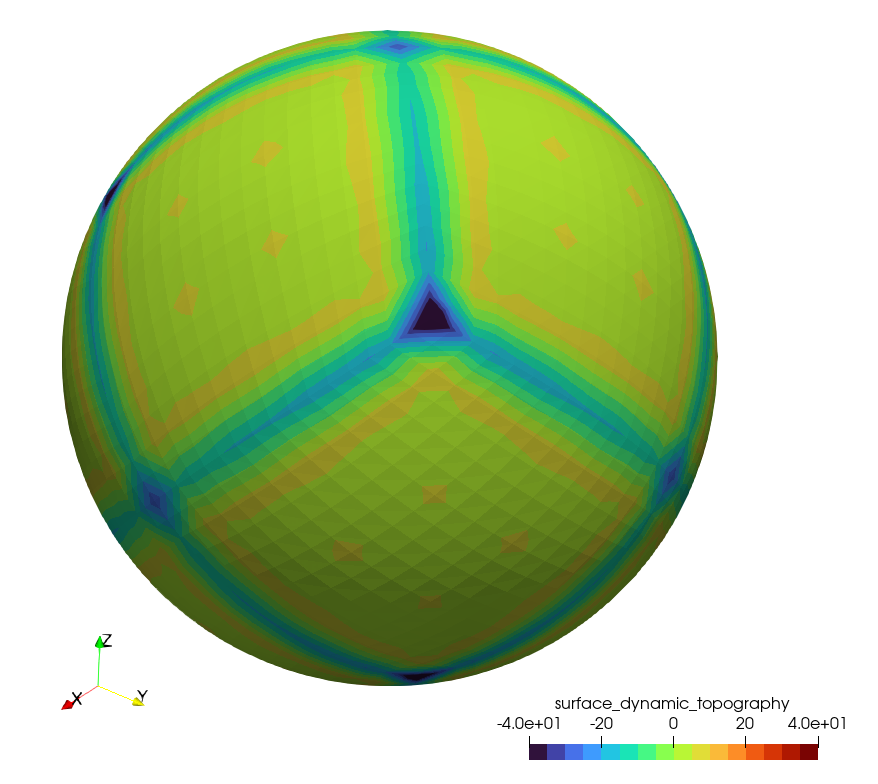
\includegraphics[width=5cm]{images/dyntopo/dyntopo.jpg}\\
{\captionfont Taken from \url{http://www.ga.gov.au/news-events/news/latest-news/dynamic-topography-of-australias-margins}}
\end{center}

\begin{small}
\begin{itemize}
\item[\nineteeneightyfive] 
\fullcite{hacr85} 
\item[\nineteeneightyseven] 
\fullcite{repa87} 
\item[\nineteenninetytwo] 
\fullcite{kiha92} 
\item[\nineteenninetythree] 
\fullcite{gurn93} \\
\fullcite{gurn93b}
\item[\nineteenninetyseven] 
\fullcite{pymi97} 
\item[\nineteenninetynine] 
\fullcite{bumo99} 
\item[\twothousand] 
\fullcite{paha00} \\
\fullcite{paha00b} 
\item[\twothousandone] 
\fullcite{pari01} 
\item[\twothousandthree] 
\fullcite{cogu03} 
\item[\twothousandseven] 
\fullcite{stei07} 
\item[\twothousandeight] 
\fullcite{mofm08} 
\item[\twothousandnine] 
\fullcite{cohu09} 
\item[\twothousandten] 
\fullcite{bofb10} \\
\fullcite{brau10} \\
\fullcite{stfh10} \\
\fullcite{shml10} 
\item[\twothousandeleven] 
\fullcite{rapy11} 
\item[\twothousandtwelve] 
\fullcite{shlm12} \\
\fullcite{zhzf12} 
\item[\twothousandthirteen] 
\fullcite{brrs13} \\
\fullcite{flgm13} 
\item[\twothousandfifteen] 
\fullcite{aupm15} \\
\fullcite{kiff15} \\
\fullcite{dali15} 
\item[\twothousandsixteen] 
\fullcite{howa16} \\
\fullcite{gvfb16} \\
\fullcite{yagu16} \\
\fullcite{stei16} \\
\fullcite{cogb16} 
\item[\twothousandseventeen] 
\fullcite{yamm17} \\
\fullcite{aumh17} \\
\fullcite{grrb17} \\
\fullcite{rubh17} \\
\fullcite{sekf17} 
\item[\twothousandeighteen] 
\fullcite{osss18} \\
\fullcite{vibc18} 
\item[\twothousandnineteen] 
\fullcite{deli19}\\
\fullcite{stco19}\\
\fullcite{davk19}\\
\fullcite{bore19}
\item[\twothousandtwenty] 
\fullcite{braf20}\\
\fullcite{kiso20}\\
\fullcite{miac20}
\item[\twothousandtwentyone] 
\fullcite{hoar21}
\item[\twothousandtwentytwo] 
\fullcite{holt22} \\
\fullcite{gurs22}
\item[\twothousandtwentythree] 
\fullcite{ropr23} \\
\fullcite{rich23} \\
\fullcite{tabs23}
\item[\twothousandtwentyfour]
\fullcite{wisa24} \\ 
\fullcite{vibb24} \\ 
\fullcite{cawc24} \\ 
\fullcite{omrp24} \\ 
\fullcite{stsb24} 
\item[\twothousandtwentyfive]
\fullcite{yawz25}
\end{itemize}
\end{small}

See also report/article written by Zhong (2018) \textcite{zhon18}

%------------------------------------------------------------------------------
%------------------------------------------------------------------------------
\section{cratons, cratonic roots}

\begin{small}
\begin{itemize}
\item[\nineteenninetyseven] 
\fullcite{bugm97} 
\item[\nineteenninetynine] 
\fullcite{drdv99} \\
\fullcite{lemo99} 
\item[\twothousand] 
\fullcite{kiri00} \\
\fullcite{lemm00} \\
\fullcite{scth00} 
\item[\twothousandone] 
\fullcite{brsh01} \\
\fullcite{drvc01} 
\item[\twothousandthree] 
\fullcite{lemm03} \\
\fullcite{wemv03} 
\item[\twothousandsix] 
\fullcite{coll06} 
\item[\twothousandeight] 
\fullcite{onlg08} 
\item[\twothousandnine] 
\fullcite{coco09} \\
\fullcite{kekj09} 
\item[\twothousandeleven] 
\fullcite{hube11}  \\
\fullcite{salo11} 
\item[\twothousandtwelve] 
\fullcite{gohg12} \\
\fullcite{gubc12} \\
\fullcite{mibe12} \\
\fullcite{yosh12} \\
\fullcite{pokb12} 
\item[\twothousandthirteen] 
\fullcite{frbm13} \\
\fullcite{gahs13} \\
\fullcite{ligw13} 
\item[\twothousandfourteen] 
\fullcite{gagb14} \\
\fullcite{wavp14} \\
\fullcite{baeg14} \\
\fullcite{comi14} \\
\fullcite{lige14} 
\item[\twothousandfifteen] 
\fullcite{wahz15} \\
\fullcite{wazh15} \\
\fullcite{tarn15} 
\item[\twothousandsixteen] 
\fullcite{wahz16} \\
\fullcite{kobc16} 
\item[\twothousandseventeen] 
\fullcite{liwg17} 
\item[\twothousandeighteen] 
\fullcite{rabw18} \\
\fullcite{bemc18} \\
\fullcite{gomb18} \\
\fullcite{webe18b} \\
\fullcite{wavp18} \\
\fullcite{lili18} \\
\fullcite{pagc19} 
\item[\twothousandtwenty] 
\fullcite{canc20} \\
\fullcite{cels20} \\
\fullcite{pegz20} \\
\fullcite{cofm20} \\
\fullcite{pagh20} 
\item[\twothousandtwentyone] 
\fullcite{becf21} \\ 
\fullcite{pelg21} \\ 
\fullcite{foon21} \\ 
\fullcite{sasa21} 
\item[\twothousandtwentytwo] 
\fullcite{canm22} \\
\fullcite{jarv22} \\ 
\fullcite{wacw22} 
\item[\twothousandtwentythree] 
\fullcite{wacp23} \\
\fullcite{gejb23} \\
\fullcite{pacb23}
\item[\twothousandtwentyfour] 
\fullcite{fuli24} \\
\fullcite{kucp24} \\
\fullcite{recf24} \\
\fullcite{comi24} \\
\fullcite{qicz24}
\end{itemize}
\end{small}

%------------------------------------------------------------------------------
%------------------------------------------------------------------------------
\section{Lithospheric stress, intra-plate stress, intra-plate deformation}
%------------------------------------------------------------------------------
%------------------------------------------------------------------------------

\begin{small}
\begin{itemize}
\item[\nineteenseventyfive] 
\fullcite{fouy75}\\
\fullcite{sosr75}
\item[\nineteenseventysix] 
\fullcite{riss76}
\item[\nineteenseventyseven] 
\fullcite{chtu77}
\item[\nineteenseventynine] 
\fullcite{riss79}
\item[\nineteeneightynine] 
\fullcite{boww89}
\item[\nineteenninetyone] 
\fullcite{worg91}
\item[\nineteenninetytwo] 
\fullcite{rich92}\\
\fullcite{wuvr92}\\
\fullcite{zoba92}\\
\fullcite{gowc92}\\
\fullcite{clko92}
\item[\nineteenninetynine] 
\fullcite{bili99}
\item[\twothousandone] 
\fullcite{stsm01}
\item[\twothousandtwo] 
\fullcite{jack02}
\item[\twothousandfour] 
\fullcite{ligu04} \\
\fullcite{buja04}
\item[\twothousandfive] 
\fullcite{timr05}
\item[\twothousandseven] 
\fullcite{hert07}
\item[\twothousandeight] 
\fullcite{bilr08}\\
\fullcite{ghhw08}\\
\fullcite{netv08}
\item[\twothousandnine] 
\fullcite{ghhf09}\\
\fullcite{nacl09}\\
\fullcite{kalb09}
\item[\twothousandten] 
\fullcite{bepo10}\\
\fullcite{yosh10}
\item[\twothousandtwelve] 
\fullcite{nalr12}\\
\fullcite{ghho12}\\
\fullcite{wagw12}
\item[\twothousandthirteen] 
\fullcite{ghhw13}
\item[\twothousandfourteen] 
\fullcite{vagw14}
\item[\twothousandseventeen] 
\fullcite{grrb17}
\item[\twothousandeighteen] 
\fullcite{osss18}\\
\fullcite{magu18}
\item[\twothousandnineteen] 
\fullcite{tamg19}
\item[\twothousandtwentyone]
\fullcite{poyd21} 
\end{itemize}
\end{small}


%--------------------------------------------------------------------
%------------------------------------------------------------------------------
\section{passive margins} 
%--------------------------------------------------------------------
%------------------------------------------------------------------------------

\begin{small}
\begin{itemize}
\item[\nineteeneightytwo] 
\fullcite{clwv82} 
\item[\nineteeneightysix] 
\fullcite{lies86} 
\item[\twothousandfive] 
\fullcite{gebi05} 
\item[\twothousandeight] 
\fullcite{clbz08} \\
\fullcite{kasb08} 
\item[\twothousandten] 
\fullcite{fasm10} \\
\fullcite{nigm10} 
\item[\twothousandeleven] 
\fullcite{rapy11} \\
\fullcite{nigm11} \\
\fullcite{brfo11} 
\item[\twothousandthirteen] 
\fullcite{mana13} \\
\fullcite{yahb13} 
\item[\twothousandfourteen] 
\fullcite{macg14} 
\item[\twothousandfifteen] 
\fullcite{gebw15} \\
\fullcite{nigo15} 
\item[\twothousandsixteen] 
\fullcite{dupm16} 
\item[\twothousandeighteen] 
\fullcite{sahf18} \\
\fullcite{mube18} \\
\fullcite{tebu18} 
\item[\twothousandnineteen] 
\fullcite{zhli19} 
\item[\twothousandtwentyone] 
\fullcite{auws21} 
\item[\twothousandtwentytwo] 
\fullcite{bagm22}
\end{itemize}
\end{small}

%------------------------------------------------------------------------------
%------------------------------------------------------------------------------
\section{Eclogites} 
%------------------------------------------------------------------------------
%------------------------------------------------------------------------------

\begin{small}
\begin{itemize}
\item[\twothousandone] 
\fullcite{dohe01} 
\item[\twothousandseven] 
\fullcite{hecb07} 
\item[\twothousandnine] 
\fullcite{agyj09} 
\item[\twothousandthirteen] 
\fullcite{arbi13} \\
\fullcite{krcu13} 
\item[\twothousandtwentytwo] 
\fullcite{wakw22}\\ 
\fullcite{yadb22} 
\end{itemize}
\end{small}


%--------------------------------------------------------------------
%------------------------------------------------------------------------------
\section{Folding, buckling} 
%--------------------------------------------------------------------
%------------------------------------------------------------------------------

\begin{small}
\begin{itemize}
\item[\nineteenseventy] 
\fullcite{ramb70} 
\item[\nineteenseventyone] 
\fullcite{ramb71} 
\item[\nineteenseventyeight] 
\fullcite{wilz78} 
\item[\nineteenninetyone] 
\fullcite{flet91}\\ 
\fullcite{wiwh91} 
\item[\nineteenninetythree] 
\fullcite{zhhj93} 
\item[\nineteenninetyfive] 
\fullcite{flet95} 
\item[\nineteenninetysix] 
\fullcite{zhho96} 
\item[\nineteenninetynine] 
\fullcite{nagg99}\\ 
\fullcite{bupo99} \\
\fullcite{scpo99} 
\item[\twothousandone] 
\fullcite{scpo01} \\
\fullcite{scpo01b} 
\item[\twothousandtwo] 
\fullcite{mumh02} 
\item[\twothousandthree] 
\fullcite{ribe03} \\
\fullcite{nagv03} 
\item[\twothousandsix] 
\fullcite{frsc06} 
\item[\twothousandseven] 
\fullcite{risr07} 
\item[\twothousandeight] 
\fullcite{schm08} \\
\fullcite{manc08} \\
\fullcite{scdk08} 
\item[\twothousandnine] 
\fullcite{simp09} 
\item[\twothousandten] 
\fullcite{resb10} 
\item[\twothousandeleven] 
\fullcite{freh11} 
\item[\twothousandtwelve] 
\fullcite{reds12} \\
\fullcite{grsc12} \\
\fullcite{scsc12} 
\item[\twothousandthirteen] 
\fullcite{regc13} 
\item[\twothousandfourteen] 
\fullcite{freh14} \\
\fullcite{frex14} 
\item[\twothousandsixteen] 
\fullcite{frsc16} 
\item[\twothousandtwentyone] 
\fullcite{nafo21} 
\item[\twothousandtwentythree] 
\fullcite{dosk23} 
\end{itemize}
\end{small}

%--------------------------------------------------------------------
%------------------------------------------------------------------------------
\section{geoid}
%--------------------------------------------------------------------
%------------------------------------------------------------------------------

\begin{small}
\begin{itemize}
\item[\nineteeneightyfour] 
\fullcite{davi84} \\
\fullcite{hage84} \\
\fullcite{riff84} \\
\fullcite{riha84} \\
\fullcite{wari84} 
\item[\nineteeneightyfive] 
\fullcite{hacr85}\\ 
\fullcite{chas85} 
\item[\nineteeneightysix] 
\fullcite{davi86} 
\item[\nineteeneightyseven] 
\fullcite{fope87} 
\item[\nineteeneightyeight] 
\fullcite{besz88} \\
\fullcite{fope88} 
\item[\nineteeneightynine] 
\fullcite{rivf89} \\
\fullcite{hari89}
\item[\nineteenninetyone] 
\fullcite{mocf91}
\item[\nineteenninetytwo] 
\fullcite{zhgu92} \\
\fullcite{kiha92} \\
\fullcite{ribe92} 
\item[\nineteenninetythree] 
\fullcite{zhch93} \\
\fullcite{rirl93} 
\item[\nineteenninetyfour] 
\fullcite{kiha94} 
\item[\nineteenninetyfive] 
\fullcite{king95} \\
\fullcite{pape95} \\
\fullcite{mopa95} \\
\fullcite{thmc95} 
\item[\nineteenninetysix]  
\fullcite{mogu96} \\
\fullcite{kafl96} \\
\fullcite{pape96} \\
\fullcite{dofm96} \\
\fullcite{pahf96} 
\item[\nineteenninetyseven] 
\fullcite{wean97a} \\
\fullcite{king97} \\
\fullcite{thri97} 
\item[\nineteenninetyeight] 
\fullcite{cava98} \\
\fullcite{chki98} \\
\fullcite{kike98} 
\item[\twothousand] 
\fullcite{dofl00} \\
\fullcite{kafl00} \\
\fullcite{paha00} 
\item[\twothousandone] 
\fullcite{zhon01} 
\item[\twothousandtwo] 
\fullcite{peso02} 
\item[\twothousandseven] 
\fullcite{kart07} 
\item[\twothousandeight] 
\fullcite{meco08} 
\item[\twothousandnine] 
\fullcite{king09} \\
\fullcite{tocm09} \\
\fullcite{yona09} 
\item[\twothousandten] 
\fullcite{ghbz10}\\
\fullcite{spgs10b}
\item[\twothousandeleven] 
\fullcite{capd11}
\item[\twothousandtwelve] 
\fullcite{hibi12}\\
\fullcite{cabp12}\\
\fullcite{katr12}
\item[\twothousandthirteen] 
\fullcite{shsc13}\\
\fullcite{chus13}
\item[\twothousandfourteen] 
\fullcite{cako14}\\
\fullcite{kaps14}
\item[\twothousandfifteen] 
\fullcite{lizh15}
\item[\twothousandsixteen] 
\fullcite{necg16}
\fullcite{lizh16}
\item[\twothousandseventeen] 
\fullcite{grab17}\\
\fullcite{siag17}
\item[\twothousandeighteen] 
\fullcite{king18}
\item[\twothousandtwentyone]
\fullcite{mazh21b} 
\item[\twothousandtwentytwo]
\fullcite{rojy22}\\
\fullcite{ghpa22}\\
\fullcite{licw22}
\item[\twothousandtwentythree]
\fullcite{stgl23} \\
\fullcite{saaf23} \\
\fullcite{pagh23}
\end{itemize}
\end{small}

%--------------------------------------------------------------------
%------------------------------------------------------------------------------
\section{geothermal Energy} 
%--------------------------------------------------------------------
%------------------------------------------------------------------------------

\begin{small}
\begin{itemize}
\item[\twothousandfifteen]
\fullcite{quxm15} 
\item[\twothousandnineteen]
\fullcite{revf19} 
\end{itemize}
\end{small}

%--------------------------------------------------------------------
%------------------------------------------------------------------------------
\section{grain size (evolution) \& influence on geodynamics}
\label{sec:topics:gsev}
%--------------------------------------------------------------------
%------------------------------------------------------------------------------

\begin{small}
\begin{itemize}
\item[\nineteeneightyfour] 
\fullcite{kara84} 
\item[\nineteenninetysix] 
\fullcite{solo96} 
\item[\nineteenninetyseven] 
\fullcite{kayf97} 
\item[\nineteeneightynine] 
\fullcite{brcp99} 
\item[\twothousandone] 
\fullcite{dets01} \\
\fullcite{solo01} 
\item[\twothousandtwo] 
\fullcite{soet02} 
\item[\twothousandthree] 
\fullcite{hapa03} \\
\fullcite{reyu03} 
\item[\twothousandeight] 
\fullcite{sore08} 
\item[\twothousandnine] 
\fullcite{behe09} 
\item[\twothousandeleven] 
\fullcite{rorb11} 
\item[\twothousandtwelve]
\fullcite{fobl12} 
\item[\twothousandthirteen] 
\fullcite{beri13} 
\item[\twothousandfourteen] 
\fullcite{fobe14} 
\item[\twothousandfifteen] 
\fullcite{thrk15} \\
\fullcite{besr15} \\
\fullcite{tukb15} \\
\fullcite{pevp15} \\
\fullcite{glfa15} 
\item[\twothousandseventeen] 
\fullcite{ceww17} \\
\fullcite{daef17} \\
\fullcite{mube17} \\
\fullcite{fori17} \\
\fullcite{scdu17} 
\item[\twothousandeighteen] 
\fullcite{bemu18} \\
\fullcite{bezb18} \\
\fullcite{mube18} \\
\fullcite{jakk18} \\
\fullcite{fole18} 
\item[\twothousandnineteen] 
\fullcite{mube19} 
\item[\twothousandtwenty] 
\fullcite{mube20} \\
\fullcite{scrt20}\\
\fullcite{sctr20} \\
\fullcite{thsc20} \\
\fullcite{fole20} \\
\fullcite{sctp20} 
\item[\twothousandtwentyone]
\fullcite{mazh21a}  \\ 
\fullcite{fube21} 
\item[\twothousandtwentytwo]
\fullcite{rutb22} 
\item[\twothousandtwentythree]
\fullcite{racs23} 
\item[\twothousandtwentyfour]
\fullcite{pagr24} 
\end{itemize}
\end{small}

%--------------------------------------------------------------------
%------------------------------------------------------------------------------
\section{LLSVP, ULVZ, CMB layer, thermo-chemical piles, D'' layer}
%------------------------------------------------------------------------------
%--------------------------------------------------------------------

\begin{center}
\includegraphics[width=5cm]{images/burk11}\cite{burk11}
\end{center}

\begin{small}
\begin{itemize}
\item[\nineteeneighty]       
\fullcite{yupe80} 
\item[\nineteeneightysix]    
\fullcite{dagu86} 
\item[\nineteeneightyeight]  
\fullcite{hayu88} 
\item[\nineteeneightynine]   
\fullcite{hayu89} 
\item[\nineteenninetyfour]   
\fullcite{ride94} 
\item[\nineteenninetysix]    
\fullcite{boeh96} 
\item[\nineteenninetyseven]  
\fullcite{kell97} 
\item[\nineteenninetyeight]  
\fullcite{tack98b} 
\item[\twothousand]
\fullcite{moke00} 
\item[\twothousandone]       
\fullcite{soga01} 
\item[\twothousandtwo]       
\fullcite{somo02} \\
\fullcite{tagh02} 
\item[\twothousandthree]
\fullcite{zhha03}
\item[\twothousandfour]      
\fullcite{mczh04} \\
\fullcite{nata04} 
\item[\twothousandfive]      
\fullcite{nata05} \\
\fullcite{wyso05} \\
\fullcite{mczh05a} \\
\fullcite{nata05b}
\item[\twothousandsix]       
\fullcite{nata06} 
\item[\twothousandseven]     
\fullcite{heta07}\\
\fullcite{moyu07} \\
\fullcite{pelt07} \\
\fullcite{hibl07} \\
\fullcite{yumc07} 
\item[\twothousandeight]     
\fullcite{gamc08} \\
\fullcite{nata08} \\
\fullcite{stho08} 
\item[\twothousandnine]
\fullcite{bumr09} 
\item[\twothousandten]
\fullcite{stto10} \\
\fullcite{mcgr10} \\
\fullcite{nata10} \\
\fullcite{vady10} \\
\fullcite{toyc10} 
\item[\twothousandeleven]    
\fullcite{bowg11} \\
\fullcite{talz11} \\
\fullcite{vayj11} \\
\fullcite{dekt11} \\
\fullcite{burk11} 
\item[\twothousandtwelve]    
\fullcite{stto12} \\
\fullcite{dagd12} \\
\fullcite{dect12} 
\item[\twothousandthirteen]  
\fullcite{limc13} \\
\fullcite{bogs13a} \\
\fullcite{bogs13b} 
\item[\twothousandfourteen]  
\fullcite{budt14} \\
\fullcite{lidt14} \\
\fullcite{tovd14} 
\item[\twothousandfifteen]   
\fullcite{musd15} \\
\fullcite{hafg15} \\
\fullcite{delt15} \\
\fullcite{wilm15} \\
\fullcite{lidt15} \\
\fullcite{sobd15} \\
\fullcite{dagl15} 
\item[\twothousandsixteen]   
\fullcite{dost16} \\
\fullcite{tosa16} 
\item[\twothousandseventeen] 
\fullcite{hish17} \\
\fullcite{lizh17} \\
\fullcite{limg17} \\
\fullcite{siag17} 
\item[\twothousandeighteen]  
\fullcite{daga18} \\
\fullcite{lizo18} \\
\fullcite{hect18} \\
\fullcite{dert18} 
\item[\twothousandnineteen]  
\fullcite{hebo19} \\
\fullcite{rejv19} \\
\fullcite{mcna19} 
\item[\twothousandtwenty]    
\fullcite{cilw20} \\
\fullcite{szes20} \\
\fullcite{scrt20} \\
\fullcite{daro20} \\
\fullcite{hect20b} 
\item[\twothousandtwentyone]
\fullcite{cafb21} \\
\fullcite{damg21} 
\item[\twothousandtwentytwo] 
\fullcite{limc22} \\
\fullcite{yuli22} \\
\fullcite{flbw22}\\
\fullcite{lalt22}\\
\fullcite{hulz22} 
\item[\twothousandtwentythree] 
\fullcite{hagl23} \\
\fullcite{gudl23} \\
\fullcite{padm23} \\
\fullcite{lizl23}
\item[\twothousandtwentyfour] 
\fullcite{bero24} \\
\fullcite{shml24} \\
\fullcite{liwg24} \\
\fullcite{deba24} \\
\fullcite{roy}
\item[\twothousandtwentyfive] 
\fullcite{padk25} \\
\fullcite{hedg25} \\
\fullcite{rosf25} \\
\fullcite{hugu25}
\end{itemize}
\end{small}

%--------------------------------------------------------------------
%------------------------------------------------------------------------------
\section{magma ocean}
%--------------------------------------------------------------------
%------------------------------------------------------------------------------

\begin{small}
\begin{itemize}
\item[\nineteenninetythree] 
\fullcite{sost93a} \\
\fullcite{sost93b} 
\item[\twothousandtwo] 
\fullcite{elvh02} 
\item[\twothousandsix] 
\fullcite{hosh06}
\item[\twothousandseven] 
\fullcite{solo07} 
\item[\twothousandten] 
\fullcite{devv10} 
\item[\twothousandtwelve] 
\fullcite{ullc12} 
\item[\twothousandthirteen] 
\fullcite{plth13} \\
\fullcite{moha13} 
\item[\twothousandfifteen] 
\fullcite{maha15} 
\item[\twothousandseventeen] 
\fullcite{mats17} \\ 
\fullcite{bori17} 
\item[\twothousandtwenty] 
\fullcite{bobm20} \\
\fullcite{agml20} 
\item[\twothousandtwentythree] 
\fullcite{sasa23} 
\item[\twothousandtwentyfive] 
\fullcite{bobs25} 
\end{itemize}
\end{small}

%------------------------------------------------------------------------------
%------------------------------------------------------------------------------
\section{magmatic arcs, arc volcanism}
%------------------------------------------------------------------------------
%------------------------------------------------------------------------------

\begin{small}
\begin{itemize}
\item[1982] \fullcite{crpi82}
\item[2015] \fullcite{cudd15}
\item[2017] \fullcite{sche17}\\ \fullcite{lewa17}
\item[2025] \fullcite{masg25}
\end{itemize}
\end{small}



%------------------------------------------------------------------------------
%------------------------------------------------------------------------------
\section{magma transport / melting / two-phase flow/ (intra-plate) 
volcanism / lava flow/ continental flood basalt, melt migration}
%------------------------------------------------------------------------------
%------------------------------------------------------------------------------

\begin{small}
\begin{itemize}
\item[\nineteeneightyfour] 
\fullcite{scst84} \\
\fullcite{mcke84} 
\item[\nineteeneightyfive] 
\fullcite{ribe85} \\
\fullcite{ribe85b} 
\item[\nineteeneightysix] 
\fullcite{scst86} \\
\fullcite{ribe86} 
\item[\nineteeneightyseven] 
\fullcite{hayu87} \\
\fullcite{spmc87} \\
\fullcite{rism87} \\
\fullcite{ribe87} 
\item[\nineteeneightyeight] 
\fullcite{scot88} \\
\fullcite{ribe88b} 
\item[\nineteeneightynine]
\fullcite{scst89} 
\item[\nineteenninety] 
\fullcite{hayu90} 
\item[\nineteenninetythree] 
\fullcite{spie93} \\
\fullcite{tast93} 
\item[\nineteenninetyfour] 
\fullcite{jhpp94} \\
\fullcite{sawy94} 
\item[\nineteenninetyfive] 
\fullcite{bisc95} \\
\fullcite{crks95} \\
\fullcite{ahwk95} 
\item[\nineteenninetysix] 
\fullcite{laki96} 
\item[\nineteenninetyeight] 
\fullcite{rabg98} 
\item[\nineteenninetynine] 
\fullcite{devv99} \\
\fullcite{momo99} 
\item[\twothousand] 
\fullcite{elha00} 
\item[\twothousandone] 
\fullcite{bers01} 
\item[\twothousandtwo] 
\fullcite{sobo02} 
\item[\twothousandthree] 
\fullcite{beri03} 
\item[\twothousandfive] 
\fullcite{onml05} \\
\fullcite{likc05} 
\item[\twothousandsix] 
\fullcite{onmm06} 
\item[\twothousandseven] 
\fullcite{srrb07} \\
\fullcite{mohb07} \\
\fullcite{elki07} \\
\fullcite{onlj07} \\
\fullcite{copb07} 
\item[\twothousandeight] 
\fullcite{hets08} \\
\fullcite{hest08} 
\item[\twothousandnine] 
\fullcite{bavi09} 
\item[\twothousandten] 
\fullcite{baiv10} \\
\fullcite{habl10} \\
\fullcite{cows10} \\
\fullcite{dekc10} 
\item[\twothousandeleven] 
\fullcite{baiv11} \\
\fullcite{zhgy11} \\
\fullcite{zhgh11} \\
\fullcite{bics11} \\
\fullcite{mobh11} 
\item[\twothousandtwelve] 
\fullcite{yatd12} \\
\fullcite{kasc12b} \\
\fullcite{ullc12} \\
\fullcite{plsp12} \\
\fullcite{kawe12} 
\item[\twothousandthirteen] 
\fullcite{kemk13} \\
\fullcite{mofm13} \\
\fullcite{plbs13} \\
\fullcite{mowe13} 
\item[\twothousandfourteen] 
\fullcite{kast14} 
\item[\twothousandfifteen] 
\fullcite{tukb15} \\
\fullcite{moba15} \\
\fullcite{rerl15} \\
\fullcite{riag15} \\
\fullcite{rey15} \\
\fullcite{yadm15} 
\item[\twothousandsixteen] 
\fullcite{keka16} \\
\fullcite{vade16} \\
\fullcite{mesj16} \\
\fullcite{dalg16} \\
\fullcite{libz16} \\
\fullcite{rogj16} \\
\fullcite{porb16} 
\item[\twothousandseventeen] 
\fullcite{dilc17} \\
\fullcite{arca17} \\
\fullcite{mova17} \\
\fullcite{mosw17} 
\item[\twothousandeighteen] 
\fullcite{mova18} \\
\fullcite{lorg18} \\
\fullcite{scmo18} \\ 
\fullcite{yaca18} \\ 
\fullcite{pegp18} \\ 
\fullcite{govo18} \\ 
\fullcite{shi_thesis}
\item[\twothousandnineteen] 
\fullcite{dagg19} \\
\fullcite{scmw19} \\
\fullcite{kesu19} \\
\fullcite{cerk19} \\
\fullcite{likk19} \\
\fullcite{jart19b} 
\item[\twothousandtwenty] 
\fullcite{siss20} \\
\fullcite{zhbp20} \\
\fullcite{rubk20} \\
\fullcite{rukb20} \\
\fullcite{cobd20} \\
\fullcite{spkh20} \\ 
\fullcite{spkh20b} \\ 
\fullcite{lerm20} 
\item[\twothousandtwentyone] 
\fullcite{dudm21} \\
\fullcite{damg21} 
\item[\twothousandtwentytwo] 
\fullcite{kajr22} \\
\fullcite{zhlz22} \\
\fullcite{bepp22} \\
\fullcite{vacd22} \\
\fullcite{kilk22} \\
\fullcite{kosl22}
\item[\twothousandtwentythree]
\fullcite{kimk23} \\ 
\fullcite{scmw23} \\ 
\fullcite{xumm23} \\
\fullcite{mahs23} \\
\fullcite{yole23}
\item[\twothousandtwentyfour] 
\fullcite{lumh24} \\
\fullcite{hesc24} \\
\fullcite{lech24} \\
\fullcite{mori24} \\
\fullcite{tibi24} 
\item[2025]
\fullcite{puld25}
\end{itemize}
\end{small}

%--------------------------------------------------------------------
%--------------------------------------------------------------------
\section{magma chambers}
%--------------------------------------------------------------------
%--------------------------------------------------------------------

\begin{small}
\begin{itemize}
\item[\nineteeneightytwo] 
\fullcite{spyk82} 
\item[\nineteeneightyseven] 
\fullcite{hayu87} 
\item[\twothousandfour] 
\fullcite{geys04} 
\item[\twothousandnine] 
\fullcite{vesc09} 
\item[\twothousandtwelve] 
\fullcite{gerb12} \\
\fullcite{gech12} 
\item[\twothousandfourteen] 
\fullcite{cuwi14} 
\item[\twothousandeighteen] 
\fullcite{gehn18} 
\end{itemize}
\end{small}

%--------------------------------------------------------------------
%------------------------------------------------------------------------------
\section{mantle convection/dynamics, whole Earth models, plate interaction}
%--------------------------------------------------------------------
%------------------------------------------------------------------------------

\begin{small}
\begin{itemize}
\item[\nineteensixtyseven] 
\fullcite{tuox67} 
\item[\nineteensixtynine] 
\fullcite{tuox69} 
\item[\nineteenseventyone] 
\fullcite{totu71b} \\
\fullcite{totu71} \\
\fullcite{buwh71} 
\item[\nineteenseventytwo] 
\fullcite{pelt72} \\ 
\fullcite{hstt72} \\ 
\fullcite{sctu72} 
\item[\nineteenseventythree] 
\fullcite{mcrw73} \\ 
\fullcite{rich73b} 
\item[\nineteenseventyfour] 
\fullcite{youn74} \\
\fullcite{tuht74} \\
\fullcite{trol94}\\
\fullcite{mcrw74} 
\item[\nineteenseventyfive] 
\fullcite{hemw75} \\
\fullcite{buss75} 
\item[\nineteenseventysix] 
\fullcite{mcri76} \\
\fullcite{patt76} \\
\fullcite{sath76} 
\item[\nineteenseventyseven] 
\fullcite{yusc77} 
\item[\nineteenseventyeight] 
\fullcite{mahz78} \\
\fullcite{hsui78} \\
\fullcite{haoc78} \\
\fullcite{pamc78} \\
\fullcite{jaco78} \\
\fullcite{rimc78} 
\item[\nineteenseventynine] 
\fullcite{ludt79} \\
\fullcite{buss79} \\
\fullcite{shpe79} \\
\fullcite{phiv79} 
\item[\nineteeneighty] 
\fullcite{olco80} \\
\fullcite{jamc80} \\
\fullcite{scsc80} \\
\fullcite{zess80} \\
\fullcite{daly80} 
\item[\nineteeneightyone] 
\fullcite{yups81} \\
\fullcite{buss81} \\
\fullcite{jasc81} \\
\fullcite{jape81} \\
\fullcite{haoc81} \\
\fullcite{rimc81} \\
\fullcite{cotu81} 
\item[\nineteeneightytwo] 
\fullcite{jape82} \\
\fullcite{jasc82} \\
\fullcite{homc82} \\
\fullcite{buri82} 
\item[\nineteeneightythree] 
\fullcite{hous83} \\
\fullcite{hous83b} \\
\fullcite{chri83} \\
\fullcite{chri83b} \\
\fullcite{mcke83} \\
\fullcite{boss83} \\
\fullcite{zesd83} 
\item[\nineteeneightyfour] 
\fullcite{olyb84} \\
\fullcite{jarv84} \\
\fullcite{haeb84} \\
\fullcite{haeb84b} \\
\fullcite{harp84} \\
\fullcite{davi84} \\
\fullcite{boas84} \\
\fullcite{chri84} \\
\fullcite{chri84b} \\
\fullcite{moca84}\\
\fullcite{flyu84} \\
\fullcite{jarv84} \\
\fullcite{flyu84b} 
\item[\nineteeneightyfive] 
\fullcite{jarv85} \\
\fullcite{baum85} \\
\fullcite{chri85} \\
\fullcite{csra85} \\
\fullcite{scan85} 
\item[\nineteeneightysix] 
\fullcite{davi86} \\
\fullcite{guda86} \\
\fullcite{quys86} \\
\fullcite{jape86} \\
\fullcite{crmc86} 
\item[\nineteeneightyseven] 
\fullcite{yuqh87} \\ 
\fullcite{olso87} \\ 
\fullcite{mija87} \\ 
\fullcite{chri87b} 
\item[\nineteeneightyeight] 
\fullcite{haeb88} \\
\fullcite{glat88} \\
\fullcite{gurn88} \\
\fullcite{viyu88} \\
\fullcite{whit88} \\
\fullcite{davi88} \\
\fullcite{csrr88} \\
\fullcite{elsc88} \\
\fullcite{grpa98} 
\item[\nineteeneightynine] 
\fullcite{weoy89} \\
\fullcite{chyu89} \\
\fullcite{besg89} \\
\fullcite{schm89} \\
\fullcite{sthe89} \\
\fullcite{rivi89} \\
\fullcite{chri89b} \\
\fullcite{jami89} \\
\fullcite{davi89} 
\item[\nineteenninety] 
\fullcite{trab90} \\
\fullcite{gurn90} \\
\fullcite{ketu90} \\
\fullcite{jape90} \\
\fullcite{sope90} 
\item[\nineteenninetyone] 
\fullcite{jarv91} \\
\fullcite{chha91} \\
\fullcite{mawe91} \\
\fullcite{gaot91} \\
\fullcite{vayv91} \\
\fullcite{hayk91} \\
\fullcite{leys91} \\
\fullcite{virf91} \\
\fullcite{mayu91} 
\item[\nineteenninetytwo] 
\fullcite{dari92} \\
\fullcite{besg92} \\
\fullcite{vayv92} \\
\fullcite{chri92} \\
\fullcite{haym92} \\
\fullcite{rien92} \\
\fullcite{hayk92} \\
\fullcite{mayw92} \\
\fullcite{mayu92} 
\item[\nineteenninetythree] 
\fullcite{bayr93} \\
\fullcite{zhch93} \\
\fullcite{jarv93} \\
\fullcite{tack93} \\
\fullcite{carm93} \\
\fullcite{vavy93} \\
\fullcite{tasg93} \\
\fullcite{zhgu93} \\
\fullcite{mamc93} \\
\fullcite{zebi93} \\
\fullcite{vayv93} \\
\fullcite{hayk93} \\
\fullcite{hayu93} \\
\fullcite{hoyb93} \\
\fullcite{hoby93} 
\item[\nineteenninetyfour] 
\fullcite{yurb94} \\
\fullcite{bayu94} \\
\fullcite{haeb94} \\
\fullcite{bucc94} \\
\fullcite{chho94} \\
\fullcite{tasg94} \\
\fullcite{past94} \\
\fullcite{itki94} \\
\fullcite{leka94} \\
\fullcite{sope94} \\
\fullcite{sope94b} \\
\fullcite{jarv94} \\
\fullcite{vaja94} \\
\fullcite{scha94} 
\item[\nineteenninetyfive] 
\fullcite{styu95} \\
\fullcite{bayr95} \\
\fullcite{bayr95b} \\
\fullcite{zhgu95} \\
\fullcite{vayv95} \\
\fullcite{buba95} \\
\fullcite{rasz95} \\
\fullcite{guja95} \\
\fullcite{berc95} \\
\fullcite{puhj95} \\
\fullcite{pujh95} \\
\fullcite{solo95} \\
\fullcite{vayu95} \\
\fullcite{matb95} \\
\fullcite{vayp95} \\
\fullcite{jagv95} \\
\fullcite{jarv95} \\
\fullcite{thmc95} 
\item[\nineteenninetysix] 
\fullcite{laym96} \\
\fullcite{zhyu96} \\
\fullcite{hond96} \\
\fullcite{rytr96a}\\
\fullcite{rytr96b}\\
\fullcite{tack96}\\
\fullcite{trbo96} \\
\fullcite{birg96} \\
\fullcite{burb96} \\
\fullcite{kafo96} \\
\fullcite{guez96} \\
\fullcite{vayu96} \\
\fullcite{rasz96} \\
\fullcite{rasz96b} \\
\fullcite{leka96} \\
\fullcite{iwas96} \\
\fullcite{buri96} \\
\fullcite{schh96} \\
\fullcite{mora96} \\
\fullcite{trha96} 
\item[\nineteenninetyseven] 
\fullcite{deja97} \\
\fullcite{hond97} \\
\fullcite{iwho97} \\
\fullcite{burb97} \\
\fullcite{mole97} \\
\fullcite{somo97} \\
\fullcite{rats97} \\
\fullcite{cicv97} \\
\fullcite{vayu97} \\
\fullcite{laym97} \\
\fullcite{mebr97} \\
\fullcite{csyu97} \\
\fullcite{wahe97} \\
\fullcite{dofc97} 
\item[\nineteenninetyeight] 
\fullcite{ande98} \\
\fullcite{iwho98} \\
\fullcite{devv98} \\
\fullcite{tack98} \\
\fullcite{tack98b} \\
\fullcite{trha98b} \\
\fullcite{trha98} \\
\fullcite{burl98} \\
\fullcite{mokm98} \\
\fullcite{lena98} \\
\fullcite{vayu98} \\
\fullcite{wema98} \\
\fullcite{vaba98} 
\item[\nineteenninetynine] 
\fullcite{resb99} \\
\fullcite{duyr99} \\
\fullcite{vazh99} \\
\fullcite{dava99} \\
\fullcite{tabg99} \\
\fullcite{como99} \\
\fullcite{cicv99} \\
\fullcite{trrj99} \\
\fullcite{loga99} \\
\fullcite{sola99} \\
\fullcite{momo99} 
\item[\twothousand] 
\fullcite{albe00} \\
\fullcite{hayu00} \\
\fullcite{devv00b} \\
\fullcite{tack00} \\
\fullcite{tack00b} \\
\fullcite{tack00c} \\
\fullcite{tack00d} \\
\fullcite{zhzm00} \\
\fullcite{legm00} \\
\fullcite{conr00} \\
\fullcite{somo00} \\
\fullcite{duyu00} \\
\fullcite{duyy00} 
\item[\twothousandone] 
\fullcite{vank01} \\
\fullcite{riyb01} \\
\fullcite{lemo01} \\
\fullcite{vays01} \\
\fullcite{moqu01} \\
\fullcite{zhon01} \\
\fullcite{burm01} \\
\fullcite{dabu01} 
\item[\twothousandtwo] 
\fullcite{tasu02} \\
\fullcite{modm02} \\
\fullcite{tack02} \\
\fullcite{vaya02} \\
\fullcite{vayu02} \\
\fullcite{taxi02} \\
\fullcite{scbh02} \\
\fullcite{strb02} \\
\fullcite{duyr02} \\
\fullcite{hiys02} \\
\fullcite{alva02} 
\item[\twothousandthree] 
\fullcite{hapa03} \\
\fullcite{lemo03} \\
\fullcite{mumc03} \\
\fullcite{fasa03} \\
\fullcite{heta03} \\
\fullcite{sibu03} \\
\fullcite{ogaw03} \\
\fullcite{ogaw03b} \\
\fullcite{kore03} 
\item[\twothousandfour] 
\fullcite{thkl04} \\
\fullcite{vavv04b} \\
\fullcite{xita04b} \\
\fullcite{xita04} \\
\fullcite{nata04b} \\
\fullcite{vayr04} \\
\fullcite{brws04} \\
\fullcite{stsh04} \\
\fullcite{scbh04} \\
\fullcite{wahb04} \\
\fullcite{leda04} \\
\fullcite{leda04b} 
\item[\twothousandfive]
\fullcite{resb05}\\
\fullcite{wahb05} \\
\fullcite{taxn05}\\
\fullcite{bupc05} \\
\fullcite{grlt05} \\
\fullcite{lemj05} \\
\fullcite{kogk05} \\
\fullcite{mczh05b}\\
\fullcite{vary05} \\
\fullcite{nata05} \\
\fullcite{nabu05} \\
\fullcite{chob05} \\
\fullcite{phbu05} \\
\fullcite{hosh05} \\
\fullcite{funk05} 
\item[\twothousandsix] 
\fullcite{soba06} \\
\fullcite{beck06} \\
\fullcite{nake06} \\
\fullcite{losh06} \\
\fullcite{sthh06} \\
\fullcite{yoka06} \\
\fullcite{wahb06} \\
\fullcite{gowh06} 
\item[\twothousandseven] 
\fullcite{ghja07} \\
\fullcite{nake07} \\
\fullcite{mayu07} \\
\fullcite{brva07a} \\
\fullcite{brva07b} \\
\fullcite{grlt07} \\
\fullcite{grlt07b}\\
\fullcite{huda07} \\
\fullcite{tanh07} \\
\fullcite{tagu07} \\
\fullcite{jalo07} \\
\fullcite{galo07} \\
\fullcite{galo07b} \\
\fullcite{nelo07} \\
\fullcite{soba07} 
\item[\twothousandeight] 
\fullcite{ghja08} \\
\fullcite{tack08} \\
\fullcite{tack08b} \\
\fullcite{chhl08} \\
\fullcite{brhv08} \\
\fullcite{deta08} \\
\fullcite{plva08} \\
\fullcite{hole08} \\
\fullcite{vata08} \\
\fullcite{trkr08} \\
\fullcite{shlj08} \\
\fullcite{stha08} \\
\fullcite{yosh08} \\
\fullcite{galg08} 
\item[\twothousandnine] 
\fullcite{wodd09} \\
\fullcite{fobe09} \\
\fullcite{gows09} \\
\fullcite{deta09} \\
\fullcite{onlj09} \\
\fullcite{wazh09} \\
\fullcite{vavv09} \\
\fullcite{brha09} \\
\fullcite{scbs09b} \\
\fullcite{oebm09} \\
\fullcite{fuog09} 
\item[\twothousandten] 
\fullcite{oflo10} \\
\fullcite{bumb10} \\
\fullcite{detn10} \\
\fullcite{yayh10} \\
\fullcite{nata10} \\
\fullcite{hole10} \\
\fullcite{zhzl10} \\
\fullcite{vayb10} \\
\fullcite{brmw10} 
\item[\twothousandeleven] 
\fullcite{yutc11} \\
\fullcite{lowm11} \\
\fullcite{rota11} \\
\fullcite{woda11} \\
\fullcite{lemj11} \\
\fullcite{befa11} \\
\fullcite{pewb11} \\
\fullcite{andl11}
\item[\twothousandtwelve] 
\fullcite{bisa12} \\
\fullcite{cort12b} \\
\fullcite{deyt12} \\
\fullcite{solo12}\\
\fullcite{wele12} 
\item[\twothousandthirteen] 
\fullcite{holj13}\\
\fullcite{dadb13}\\
\fullcite{toyd13}\\
\fullcite{bogs13a} \\
\fullcite{busa13} \\
\fullcite{mika13} \\
\fullcite{fabc13} \\
\fullcite{cosr13} \\
\fullcite{coml13} \\
\fullcite{cost13} \\
\fullcite{stha13} \\
\fullcite{plth13} \\
\fullcite{oflb13} \\
\fullcite{whch13} 
\item[\twothousandfourteen] 
\fullcite{arfw14} \\
\fullcite{helo14} \\
\fullcite{crta14} \\
\fullcite{flgw14} \\
\fullcite{roct14} \\
\fullcite{cort14} \\
\fullcite{becr14} \\
\fullcite{nata14} \\
\fullcite{stha14} \\
\fullcite{stlh14} \\
\fullcite{ogaw14} 
\item[\twothousandfifteen]   
\fullcite{zhru15} \\
\fullcite{wegg15} \\
\fullcite{nata15} \\
\fullcite{bect15} \\
\fullcite{pesw15} \\
\fullcite{plht15} \\
\fullcite{khfh15} 
\item[\twothousandsixteen]   
\fullcite{frbs16}  \\
\fullcite{plhm16} \\
\fullcite{boba16} \\
\fullcite{wele16} \\
\fullcite{welm16} \\
\fullcite{vade16} \\
\fullcite{chah16} \\
\fullcite{woso16b} 
\item[\twothousandseventeen] 
\fullcite{badw17} \\
\fullcite{ghts17} \\
\fullcite{civj17} 
\item[\twothousandeighteen] 
\fullcite{guld18} \\
\fullcite{arcf18} \\
\fullcite{plhw18} \\
\fullcite{wele18} 
\item[\twothousandnineteen] 
\fullcite{gult19} \\
\fullcite{mazh19} \\
\fullcite{cohf19} \\
\fullcite{lewh19} \\
\fullcite{ulcw19} \\
\fullcite{boba19} \\
\fullcite{fube19} \\
\fullcite{plju19} 
\item[\twothousandtwenty] 
\fullcite{lalt20} \\
\fullcite{gugb20} \\
\fullcite{yabt20} \\
\fullcite{yosy20} \\
\fullcite{arcf20} \\
\fullcite{babd20} \\
\fullcite{lorb20} \\
\fullcite{loru20} 
\item[\twothousandtwentyone] 
\fullcite{lalt21} \\
\fullcite{naka21} \\
\fullcite{khmo21} 
\item[\twothousandtwentytwo] 
\fullcite{lids22} \\ 
\fullcite{pade22} \\ 
\fullcite{fube22} 
\item[\twothousandtwentythree] 
\fullcite{befu23} \\ 
\fullcite{yosh23} 
\item[\twothousandtwentyfour] 
\fullcite{vavt24} \\ 
\fullcite{jalt24} \\ 
\fullcite{xihw24} \\ 
\fullcite{lobb24} 
\end{itemize}
\end{small}

%--------------------------------------------------------------------
%------------------------------------------------------------------------------
\section{mantle convection + continental growth}
%------------------------------------------------------------------------------
%--------------------------------------------------------------------

\begin{small}
\begin{itemize}
\item[1997]
\fullcite{wahe97b}
\item[1999]
\fullcite{wahe99}
\item[2007]
\fullcite{wahb07}
\item[2008]
\fullcite{wahe08} \\
\fullcite{wahb08}
\item[2009]
\fullcite{wahk09} \\
\fullcite{wahe09}
\item[2013]
\fullcite{wahe13} \\
\fullcite{wahe13b}
\item[2017]
\fullcite{wahe17}
\end{itemize}
\end{small}

%--------------------------------------------------------------------
%------------------------------------------------------------------------------
\section{mantle rheology, phase transitions, stratification, (temperature) profile}
%------------------------------------------------------------------------------
%--------------------------------------------------------------------

\begin{small}
\begin{itemize}
\item[1923] 
\fullcite{wiad23} 
\item[1952] 
\fullcite{birc52} 
\item[\nineteenseventyone] 
\fullcite{sctu71}\\ 
\fullcite{tusc71} 
\item[\nineteenseventysix] 
\fullcite{ocon76} 
\item[\nineteenseventyseven] 
\fullcite{stac77}
\item[\nineteeneightytwo] 
\fullcite{yusb82}\\
\fullcite{chri82}
\item[\nineteeneightyfive] 
\fullcite{chyu85}
\item[\nineteeneightysix] 
\fullcite{yuen86} 
\item[\nineteeneightynine] 
\fullcite{itka89} 
\item[\nineteenninetyone] 
\fullcite{fopd91} \\ 
\fullcite{mawe91}
\item[\nineteenninetytwo] 
\fullcite{zhyh92} \\
\fullcite{zhyh92}
\item[\nineteenninetythree] 
\fullcite{tasg93} \\
\fullcite{best93} \\
\fullcite{kief93} \\
\fullcite{styz93} \\
\fullcite{yucc93} \\
\fullcite{hoby93} \\
\fullcite{dayu93} 
\item[\nineteenninetyfour] 
\fullcite{cays94}\\
\fullcite{vayv94}\\
\fullcite{zhgu94b}\\
\fullcite{styu94}\\
\fullcite{sope94}\\
\fullcite{popy94}
\item[\nineteenninetyfive] 
\fullcite{kiit95}\\
\fullcite{zhyu95} \\
\fullcite{chri95}\\
\fullcite{scta95}\\
\fullcite{tack95}
\item[\nineteenninetysix] 
\fullcite{pelt96}\\
\fullcite{mitr96}\\
\fullcite{tack96b}
\item[\nineteenninetyseven] 
\fullcite{mifo97}\\
\fullcite{cica97}\\
\fullcite{pebs97}
\item[\nineteenninetyeight] 
\fullcite{cava98}\\
\fullcite{kenn98}
\item[\nineteenninetynine] 
\fullcite{sigh99} \\
\fullcite{kehv99} \\
\fullcite{vaka99} \\
\fullcite{beko99} 
\item[\twothousandone] 
\fullcite{roma01} \\
\fullcite{dest01} 
\item[\twothousandthree] 
\fullcite{beka03} \\
\fullcite{roma03} 
\item[\twothousandfive] 
\fullcite{hett05}\\
\fullcite{nata05b}\\
\fullcite{nabu05}\\
\fullcite{stli05}\\
\fullcite{stli05b}
\item[\twothousandsix] 
\fullcite{javd06}\\
\fullcite{stca06}
\item[\twothousandseven]
\fullcite{stei07} \\
\fullcite{pazw07} \\
\fullcite{mofm07} \\
\fullcite{tanh07} \\
\fullcite{stli07} \\
\fullcite{lioh07} \\
\fullcite{jade07} \\
\fullcite{pisb07} \\
\fullcite{kart07} 
\item[\twothousandnine]  
\fullcite{natd09} \\
\fullcite{conn09} 
\item[\twothousandten]   
\fullcite{mohy10} \\ 
\fullcite{kayy10} 
\item[\twothousandeleven] 
\fullcite{mayw11} \\
\fullcite{java11} \\
\fullcite{faff11} \\
\fullcite{catb11} \\
\fullcite{nata11} \\
\fullcite{vayj11} \\
\fullcite{stli11} 
\item[\twothousandtwelve] 
\fullcite{tack12}\\
\fullcite{sato12}\\
\fullcite{simj12} \\
\fullcite{natd12} \\
\fullcite{stli12} 
\item[\twothousandthirteen] 
\fullcite{fakc13}\\
\fullcite{taab13} \\
\fullcite{jasv13}
\item[\twothousandfifteen] 
\fullcite{basn15}\\
\fullcite{glfa15}\\
\fullcite{amsb15}\\
\fullcite{soyu15}\\
\fullcite{wahg15} 
\item[\twothousandsixteen] 
\fullcite{tiro16}\\
\fullcite{beci16}
\item[\twothousandseventeen] 
\fullcite{jasv17} \\
\fullcite{bahh17} \\
\fullcite{shyp17} \\
\fullcite{shpj17} \\
\fullcite{balh17} 
\item[\twothousandeighteen] 
\fullcite{vavs18} \\
\fullcite{mazh18}\\
\fullcite{naoi18}\\
\fullcite{roct18}
\item[\twothousandnineteen] 
\fullcite{jasv19} \\
\fullcite{wahg19} \\
\fullcite{sism19} 
\item[\twothousandtwenty] 
\fullcite{hohv20} \\
\fullcite{lufs20} \\
\fullcite{wali20} \\
\fullcite{ruml20} 
\item[\twothousandtwentyone] 
\fullcite{pocv21} \\
\fullcite{vepn21} \\
\fullcite{adkc21} \\
\fullcite{gath21} \\
\fullcite{ligl21b} \\
\fullcite{mazh21b} \\ 
\fullcite{gubt21} \\
\fullcite{josv21} 
\item[\twothousandtwentytwo] 
\fullcite{rikg22} \\ 
\fullcite{dagl22} \\ 
\fullcite{stli22} 
\item[\twothousandtwentythree] 
\fullcite{speg23} \\ 
\fullcite{mych23} 
\end{itemize}
\end{small}


%--------------------------------------------------------------------
%------------------------------------------------------------------------------
\section{mantle wedge, subduction zone (temperature)} 
%------------------------------------------------------------------------------
%--------------------------------------------------------------------

\begin{small}
\begin{itemize}
\item[\nineteensixtynine] 
\fullcite{mcke69} 
\item[\nineteenseventyone] 
\fullcite{tomj71} 
\item[\nineteenseventythree] 
\fullcite{toss73} 
\item[\nineteenseventyfive] 
\fullcite{bits75} 
\item[\nineteenseventyseven] 
\fullcite{tobi77} 
\item[\nineteenseventyeight] 
\fullcite{tosl78} 
\item[\nineteenseventynine] 
\fullcite{bobo79} 
\item[\nineteeneightyfive] 
\fullcite{hond85} 
\item[\nineteenninetytwo] 
\fullcite{dast92} 
\item[\nineteenninetythree] 
\fullcite{furu93} 
\item[\nineteenninetynine] 
\fullcite{pewa99} 
\item[\twothousandone] 
\fullcite{bigu01} \\
\fullcite{haki01} 
\item[\twothousandtwo]
\fullcite{vakp02} 
\item[\twothousandthree]
\fullcite{vank03} 
\item[\twothousandfour]
\fullcite{enwi04} \\
\fullcite{cuwh04} 
\item[\twothousandsix] 
\fullcite{abvk06} \\
\fullcite{gogc06} \\
\fullcite{gecy06} \\
\fullcite{syab06} \\
\fullcite{lafh06} 
\item[\twothousandseven] 
\fullcite{gogc07} \\
\fullcite{knvk07} \\
\fullcite{lohd07} 
\item[\twothousandeight]
\fullcite{knva08} \\
\fullcite{cage08} \\
\fullcite{vack08} \\
\fullcite{wawh08} 
\item[\twothousandnine] 
\fullcite{leki09} \\
\fullcite{heaa09} \\
\fullcite{wawa09} 
\item[\twothousandten]
\fullcite{roms10} \\
\fullcite{hogz10} 
\item[\twothousandeleven] 
\fullcite{zhgh11} \\
\fullcite{moho11} \\
\fullcite{wiko12}  
\item[\twothousandfourteen]
\fullcite{ledg14} \\
\fullcite{mabv14} 
\item[\twothousandfourteen]
\fullcite{wahh15} 
\item[\twothousandsixteen]
\fullcite{dalg16} \\ 
\fullcite{pegp16} 
\item[\twothousandseventeen]
\fullcite{rerm17} \\
\fullcite{mova17}
\item[\twothousandeighteen]
\fullcite{pltv18} \\ 
\fullcite{pegp18} 
\item[\twothousandtwentyone]
\fullcite{wada21} 
\item[\twothousandtwentytwo]
\fullcite{reps22} 
\item[\twothousandtwentythree]
\fullcite{izhy23} \\
\fullcite{vatc23} \\ 
\fullcite{yole23}
\item[\twothousandtwentyfour]
\fullcite{epcs24} \\
\fullcite{pebo24} 
\end{itemize}
\end{small}

\newpage
%--------------------------------------------------------------------
%------------------------------------------------------------------------------
\section{mixing, stirring, degassing, outgassing, Lyapunov exponent, volatiles } 
%------------------------------------------------------------------------------
%--------------------------------------------------------------------

\begin{small}
\begin{itemize}
\item[\nineteeneightytwo] 
\fullcite{ridn82} 
\item[\nineteeneightyfour] 
\fullcite{olyb84} \\ 
\fullcite{olyb84b} 
\item[\nineteeneightyfive] 
\fullcite{homc85} 
\item[\nineteeneightysix] 
\fullcite{altu86} \\ 
\fullcite{gurn86} \\ 
\fullcite{guda86b} \\
\fullcite{guda86c}
\item[\nineteeneightyeight] 
\fullcite{otlr88} 
\item[\nineteeneightynine] 
\fullcite{chri89} 
\item[\nineteenninety] 
\fullcite{ketu90} \\
\fullcite{davi90} 
\item[\nineteenninetyone] 
\fullcite{pier91} \\
\fullcite{kest91}
\item[\nineteenninetytwo] 
\fullcite{hayk92}
\item[\nineteenninetythree]
\fullcite{kell93} 
\item[\nineteenninetyfour]
\fullcite{scha94}
\item[\nineteenninetyfive] 
\fullcite{mebo95} \\
\fullcite{frbo95}
\item[\nineteenninetysix] 
\fullcite{pelt96}\\ 
\fullcite{teyl96}\\ 
\fullcite{mang96} 
\item[\nineteenninetyseven]
\fullcite{teyp97} \\
\fullcite{frbo97} 
\item[\nineteenninetyeight]
\fullcite{tepy98} \\
\fullcite{vaba98} 
\item[\nineteenninetynine] 
\fullcite{vazh99} \\
\fullcite{cori99} 
\item[\twothousandone] 
\fullcite{huke01} 
\item[\twothousandtwo] 
\fullcite{vahb02} \\
\fullcite{falt02}
\item[\twothousandthree] 
\fullcite{fasa03} \\
\fullcite{vabh03} 
\item[\twothousandfive] 
\fullcite{colt05} 
\item[\twothousandsix] 
\fullcite{gowh06}\\ 
\fullcite{cosc06} 
\item[\twothousandseven] 
\fullcite{gogc07} \\
\fullcite{nake07} \\
\fullcite{huda07b} \\
\fullcite{vabh07} 
\item[\twothousandten] 
\fullcite{mang10}
\item[\twothousandeleven] 
\fullcite{lemj11} \\
\fullcite{saad11} 
\item[\twothousandthirteen]
\fullcite{onlh13}
\item[\twothousandfifteen] 
\fullcite{pedp15}
\item[\twothousandeighteen] 
\fullcite{bipe18} \\
\fullcite{onzh18} 
\item[\twothousandtwentytwo] 
\fullcite{onau22} 
\item[\twothousandtwentyfour] 
\fullcite{vatv24} \\ 
\fullcite{lamt24} \\ 
\fullcite{thsf24} 
\end{itemize}
\end{small}


\newpage
%--------------------------------------------------------------------
%------------------------------------------------------------------------------
\section{mantle reservoirs, magma reservoirs}
%------------------------------------------------------------------------------
%--------------------------------------------------------------------

\begin{small}
\begin{itemize}
\item[\nineteeneightythree] 
\fullcite{mcon83}
\item[\nineteeneightyfive] 
\fullcite{homc85}
\item[\nineteeneightysix] 
\fullcite{guda86b}
\item[\nineteenninetynine] 
\fullcite{wahe99}
\item[\twothousandtwo] 
\fullcite{cori02}
\item[\twothousandfive] 
\fullcite{vavv05b}
\item[\twothousandeight]
\fullcite{wahb08}
\item[\twothousandnine] 
\fullcite{vavv09}
\item[\twothousandten] 
\fullcite{mcgr10}
\item[\twothousandeleven] 
\fullcite{wahe11}
\item[\twothousandfourteen] 
\fullcite{limg14} \\
\fullcite{lidt14}
\item[\twothousandfifteen] 
\fullcite{lidt15}
\item[\twothousandseventeen] 
\fullcite{fori17}
\item[\twothousandtwenty] 
\fullcite{pact20}
\item[\twothousandtwentytwo] 
\fullcite{lids22} \\
\fullcite{patc22}
\item[\twothousandtwentythree] 
\fullcite{gudl23}
\end{itemize}
\end{small}


\newpage
%--------------------------------------------------------------------
%--------------------------------------------------------------------
\section{micro-continents}
%--------------------------------------------------------------------
%--------------------------------------------------------------------

\begin{small}
\begin{itemize}
\item[2019] \fullcite{kobg19}
\item[2020] \fullcite{vaga20}
\item[2021] \fullcite{gupg21}
\item[2024] \fullcite{qilb24}
\item[2025] \fullcite{erbt25}
\end{itemize}
\end{small}


\newpage
%--------------------------------------------------------------------
%------------------------------------------------------------------------------
\section{Obduction, ophiolites}
%------------------------------------------------------------------------------
%--------------------------------------------------------------------

\begin{small}
\begin{itemize}
\item[\nineteenninety] 
\fullcite{hack90} 
\item[\nineteenninetyone] 
\fullcite{hack91} 
\item[\nineteenninetyseven] 
\fullcite{rabh97} 
\item[\twothousand] 
\fullcite{mokd00} 
\item[\twothousandfourteen] 
\fullcite{agzf14} 
\item[\twothousandsixteen] 
\fullcite{duay16} 
\item[\twothousandtwenty] 
\fullcite{rohb20} 
\item[\twothousandtwentyone] 
\fullcite{pody21} 
\item[\twothousandtwentytwo] 
\fullcite{zhli22} 
\end{itemize}
\end{small}

%--------------------------------------------------------------------
%--------------------------------------------------------------------
\section{oceanic Lithosphere}
%--------------------------------------------------------------------
%--------------------------------------------------------------------

\begin{small}
\begin{itemize}
\item[\nineteenseventysix] 
\fullcite{scfy76} 
\item[\nineteenseventyseven] 
\fullcite{debr77} 
\item[\nineteeneightythree] 
\fullcite{cobe83} 
\item[\nineteeneightyfour] 
\fullcite{yufl84} 
\item[\nineteeneightyeight] 
\fullcite{mofo88} 
\item[\nineteenninety] 
\fullcite{ogaw90} 
\item[\twothousand] 
\fullcite{tesc00} 
\item[\twothousandone] 
\fullcite{kasc01} 
\item[\nineteeneightyfour] 
\fullcite{flyu84} 
\item[\nineteenninetyeight] 
\fullcite{bupo98}
\item[\twothousandfive] 
\fullcite{huzh05}
\item[\twothousandseven] 
\fullcite{afrf07} \\
\fullcite{kore07} \\
\fullcite{macl07} 
\item[\twothousandeight] 
\fullcite{chgu08} \\
\fullcite{zlad08}
\item[\twothousandtwelve] 
\fullcite{trub12} 
\item[\twothousandsixteen]  
\fullcite{koko16} 
\item[\twothousandeighteen] 
\fullcite{rihc18} 
\end{itemize}
\end{small}

%--------------------------------------------------------------------
%--------------------------------------------------------------------
\section{ocean floor, seafloor}
%--------------------------------------------------------------------
%--------------------------------------------------------------------

\begin{small}
\begin{itemize}
\item[1977]
\fullcite{pasc77}
\item[1980] 
\fullcite{jape80}
\item[1981]
\fullcite{jape81}
\item[2003]
\fullcite{covb03}
\item[2008]
\fullcite{afzf08}
\item[2012]
\fullcite{cort12b}
\item[2014]
\item[2015]
\fullcite{olbi15}
\fullcite{lige15}
\end{itemize}
\end{small}


%--------------------------------------------------------------------
%--------------------------------------------------------------------
\section{onset of convection}
%--------------------------------------------------------------------
%--------------------------------------------------------------------

\begin{small}
\begin{itemize}
\item[\nineteensixtynine]
\fullcite{scto69} 
\item[\nineteeneightytwo] 
\fullcite{homc82} 
\item[\nineteenninety] 
\fullcite{sope90} 
\item[\twothousand] 
\fullcite{scth00} 
\item[\twothousandsix] 
\fullcite{soba06} 
\item[\twothousandtwo] 
\fullcite{kojo02} 
\item[\twothousandtwo] 
\fullcite{kojo03} 
\item[\twothousandseven] 
\fullcite{soba07} 
\item[\twothousandfifteen] 
\fullcite{kamo15} 
\end{itemize}
\end{small}

%--------------------------------------------------------------------
%------------------------------------------------------------------------------
\section{plate motion and mantle, plate tectonic reconstruction, mechanism}
%------------------------------------------------------------------------------
%--------------------------------------------------------------------

\begin{small}
\begin{itemize}
\item[\nineteensixtysix] 
\fullcite{wils66}
\item[\nineteensixtyseven] 
\fullcite{mcpa67}
\item[\nineteensixtyeight] 
\fullcite{isos68} 
\item[\nineteenseventythree] 
\fullcite{mcse73}
\item[\nineteenseventyfour] 
\fullcite{sosl74}
\item[\nineteenseventyfive] 
\fullcite{harp75} \\
\fullcite{turc75}
\item[\nineteenninety] 
\fullcite{dega90}
\item[\nineteenninetyone] 
\fullcite{virf91}
\item[\nineteenninetytwo] 
\fullcite{zieg92a} \\
\fullcite{gost92}
\item[\nineteenninetyfour] 
\fullcite{guto94}
\item[\nineteenninetyseven] 
\fullcite{wean97b}
\item[\nineteenninetyeight] 
\fullcite{zhgm98} \\ 
\fullcite{liri98}
\item[\nineteenninetynine] 
\fullcite{ribr99}
\item[\twothousandone] 
\fullcite{yohk01}
\item[\twothousandtwo] 
\fullcite{stoc02}
\item[\twothousandthree] 
\fullcite{evan03} \\
\fullcite{reta03}
\item[\twothousandseven] 
\fullcite{zhzl07}
\item[\twothousandnine] 
\fullcite{lizh09} \\
\fullcite{vasv09} \\
\fullcite{iabu09} \\
\fullcite{scbs09}
\item[\twothousandten] 
\fullcite{stto10} \\
\fullcite{dega10}
\item[\twothousandtwelve] 
\fullcite{huss12} \\
\fullcite{gutz12} \\
\fullcite{qumm12} \\
\fullcite{holr12} \\
\fullcite{dost12} \\
\fullcite{shbs12}
\item[\twothousandthirteen] 
\fullcite{mosq13} \\
\fullcite{cost13} 
\item[\twothousandfourteen] 
\fullcite{ruzh14} 
\item[\twothousandfifteen] 
\fullcite{yoha15}
\item[\twothousandsixteen] 
\fullcite{pric16}
\item[\twothousandseventeen] 
\fullcite{stid17}
\item[\twothousandnineteen] 
\fullcite{tewg19} \\
\fullcite{weco19} \\ 
\fullcite{flam19} 
\item[\twothousandtwenty]
\fullcite{sele20} \\
\item[\twothousandtwentyone]
\fullcite{cafm21} \\
\fullcite{atco21}
\item[\twothousandtwentyfour]
\fullcite{wefl24} 
\end{itemize}
\end{small}



%--------------------------------------------------------------------
%------------------------------------------------------------------------------
\section{plume dynamics \& shape}
%------------------------------------------------------------------------------
%--------------------------------------------------------------------

\begin{small}
\begin{itemize}
\item[\nineteenseventyone] 
\fullcite{morg71} 
\item[\nineteenseventythree] 
\fullcite{toze73} 
\item[\nineteenseventyfive] 
\fullcite{patt75} 
\item[\nineteenseventyseven] 
\fullcite{hovo77}
\item[\nineteeneighty] 
\fullcite{yupe80} 
\item[\nineteeneightyseven] 
\fullcite{zhyu87} \\
\fullcite{olsa87} \\
\fullcite{rism87} 
\item[\nineteeneightyeight] 
\fullcite{olsa88} \\
\fullcite{rigr88}
\item[\nineteeneightynine] 
\fullcite{jami89} \\
\fullcite{scoa89}
\item[\nineteenninety] 
\fullcite{davi90}
\item[\nineteenninetyone] 
\fullcite{kell91}\\
\fullcite{grca91b}
\item[\nineteenninety] 
\fullcite{grca90}
\item[\nineteenninetythree] 
\fullcite{keki93}\\
\fullcite{olsa93}\\
\fullcite{mayu93}
\item[\nineteenninetyfour] 
\fullcite{nasf94}\\
\fullcite{fari94}\\
\fullcite{leka94b}\\
\fullcite{hayu94}\\
\fullcite{mamy94}
\item[\nineteenninetyfive] 
\fullcite{fari95} \\
\fullcite{scag95}
\item[\nineteenninetysix] 
\fullcite{lesy96} 
\item[\nineteenninetyseven] 
\fullcite{vank97} \\
\fullcite{keki97}\\
\fullcite{laym97} \\
\fullcite{layu97}\\
\fullcite{layu97b}\\
\fullcite{mang97} \\
\fullcite{king97} 
\item[\nineteenninetyeight] 
\fullcite{thta98} \\ 
\fullcite{stoc98}
\item[\nineteenninetynine] 
\fullcite{lays99} \\
\fullcite{wuda99}
\item[\twothousand] 
\fullcite{csyu00}\\
\fullcite{bryu00}
\item[\twothousandone] 
\fullcite{lirc01}
\item[\twothousandtwo] 
\fullcite{falt02} \\
\fullcite{dagl02} \\
\fullcite{nitg02} \\
\fullcite{labr02} \\
\fullcite{tagh02}
\item[\twothousandthree] 
\fullcite{safa03}
\item[\twothousandfour] 
\fullcite{goch04}\\ 
\fullcite{scmo04}\\
\fullcite{lokg04}\\
\fullcite{keso04} 
\item[\twothousandfive] 
\fullcite{tagu05}\\ 
\fullcite{bung05}\\
\fullcite{zhon05}\\
\fullcite{liva05}\\
\fullcite{mayu05}
\item[\twothousandsix] 
\fullcite{isst06}\\
\fullcite{liva06a}\\
\fullcite{liva06b}\\
\fullcite{zhon06}\\ 
\fullcite{mita06}\\
\fullcite{nokm06} \\
\fullcite{qufo06} \\
\fullcite{keso06} \\
\fullcite{cada06}
\item[\twothousandseven] 
\fullcite{yumh07}\\
\fullcite{ogaw07}
\item[\twothousandeight] 
\fullcite{logg08} \\ 
\fullcite{lezh08b} 
\item[\twothousandnine] 
\fullcite{vavl09}\\
\fullcite{bogj09}\\
\fullcite{faho09}\\
\fullcite{scbs09b}\\
\fullcite{lezh09}
\item[\twothousandeleven] 
\fullcite{toyu11}\\
\fullcite{talz11}\\
\fullcite{burk11}\\
\fullcite{memm11}\\
\fullcite{dalt11}\\
\fullcite{tree11}
\item[\twothousandtwelve] 
\fullcite{viym12} 
\fullcite{legu12} 
\item[\twothousandthirteen] 
\fullcite{dagm13} \\
\fullcite{madd13} \\
\fullcite{ande13} \\
\fullcite{vadv13} \\
\fullcite{bova13} \\
\fullcite{dusm13} 
\item[\twothousandfourteen] 
\fullcite{glfo14} 
\item[\twothousandfifteen] 
\fullcite{daso15} \\
\fullcite{hafg15} \\
\fullcite{canl15} \\
\fullcite{sule15} \\
\fullcite{hels15}
\item[\twothousandsixteen] 
\fullcite{kili16}\\
\fullcite{jodc16}\\
\fullcite{shpy16}\\
\fullcite{dannbergphd}
\item[\twothousandseventeen] 
\fullcite{moyu17} \\
\fullcite{lizh17} 
\item[\twothousandeighteen] 
\fullcite{dacc18} \\
\fullcite{trev18} \\
\fullcite{zhli18} \\
\fullcite{moyu18} 
\item[\twothousandnineteen] 
\fullcite{argc19} \\
\fullcite{lizh19} 
\item[\twothousandtwenty] 
\fullcite{gugm20} \\
\fullcite{rits20} \\
\fullcite{hect20b} 
\item[\twothousandtwentyone] 
\fullcite{xiwk21} \\ 
\fullcite{levp21} 
\item[\twothousandtwentytwo] 
\fullcite{gugt22} 
\item[\twothousandtwentythree] 
\fullcite{li__23} \\
\fullcite{leli23} \\ 
\fullcite{nemi23} \\ 
\fullcite{lilw23} 
\item[\twothousandtwentyfour]
\fullcite{farn24} \\
\fullcite{roy}
\item[\twothousandtwentyfive]
\fullcite{hedg25}
\end{itemize}
\end{small}

%------------------------------------------------------------------------------
%------------------------------------------------------------------------------
\section{plume-lithosphere interaction, LIP, hotspots}
%------------------------------------------------------------------------------
%------------------------------------------------------------------------------

\begin{small}
\begin{itemize}
\item[1988]
\fullcite{olsa88}
\item[\nineteenninety] 
\fullcite{davi90} \\ 
\fullcite{hous90b} 
\item[\nineteenninetyone] 
\fullcite{grca91} 
\item[\nineteenninetytwo] 
\fullcite{hicd92} \\
\fullcite{cagr92} \\
\fullcite{sask92} 
\item[\nineteenninetyfour] 
\fullcite{rich94} \\
\fullcite{fari94} \\
\fullcite{ride94} \\
\fullcite{davi94} 
\item[\nineteenninetyfive] 
\fullcite{whmc95} \\
\fullcite{fari95} \\
\fullcite{rict95} 
\item[\nineteenninetysix] 
\fullcite{zhgm96} \\
\fullcite{ribe96} 
\item[\nineteenninetyeight] 
\fullcite{most98} \\
\fullcite{ride98} 
\item[\nineteenninetynine] 
\fullcite{most99} \\
\fullcite{shet99} \\
\fullcite{bisp99} 
\item[\twothousand] 
\fullcite{lors00} 
\item[\twothousandone] 
\fullcite{vapy01}
\item[\twothousandtwo] 
\fullcite{foul02} \\
\fullcite{labr02}
\item[\twothousandthree] 
\fullcite{vazh03} \\
\fullcite{gacs03} \\
\fullcite{codb03} 
\item[\twothousandfour] 
\fullcite{yoog04} 
\item[\twothousandfive] 
\fullcite{bugu05} \\
\fullcite{fasa05} \\
\fullcite{yoog05} \\
\fullcite{camp05} \\
\fullcite{likc05} 
\item[\twothousandsix] 
\fullcite{dabu06}\\ 
\fullcite{thtd06} 
\item[\twothousandseven] 
\fullcite{stco07} 
\item[\twothousandeight] 
\fullcite{uegs08} \\
\fullcite{slee08} 
\item[\twothousandnine] 
\fullcite{bucl09} \\
\fullcite{zhgy09} \\
\fullcite{baiv10} \\
\fullcite{tabs09} \\
\fullcite{maml09} \\
\fullcite{dada09} 
\item[\twothousandten] 
\fullcite{fabl10} \\
\fullcite{lezh10} 
\item[\twothousandeleven] 
\fullcite{sosk11} \\
\fullcite{vasd11} \\
\fullcite{kopp11} 
\item[\twothousandtwelve] 
\fullcite{huco12} \\
\fullcite{gubc12} \\
\fullcite{bemm12} 
\item[\twothousandthirteen] 
\fullcite{brps13} 
\item[\twothousandfourteen] 
\fullcite{buge14} \\
\fullcite{gery14b} \\
\fullcite{buto14} \\
\fullcite{buit14} \\
\fullcite{leli14} \\
\fullcite{limg14} \\
\fullcite{agat13} 
\item[\twothousandfifteen] 
\fullcite{bemm15} \\
\fullcite{gesb15} \\
\fullcite{kocb15} \\
\fullcite{meds15} \\
\fullcite{lile15} \\
\fullcite{medd15} \\
\fullcite{frro15} \\
\fullcite{wham15} \\
\fullcite{dags15} 
\item[\twothousandsixteen] 
\fullcite{fige16} \\
\fullcite{gadb16} \\
\fullcite{trev16} \\
\fullcite{leli16} \\
\fullcite{kobc16} 
\item[\twothousandseventeen] 
\fullcite{bahf17} \\
\fullcite{brsg17} \\
\fullcite{bekb17} \\
\fullcite{kocb17} \\
\fullcite{egim17} 
\item[\twothousandeighteen] 
\fullcite{daga18} \\
\fullcite{frkc18} \\
\fullcite{frbr18} \\
\fullcite{gomb18} 
\item[\twothousandnineteen] 
\fullcite{kobg19} \\
\fullcite{stbl19} \\
\fullcite{botb19} 
\item[\twothousandtwenty] 
\fullcite{basg20} \\
\fullcite{basg20b} \\
\fullcite{fiog20} \\
\fullcite{dazl20} \\
\fullcite{pikw20} 
\item[\twothousandtwentyone] 
\fullcite{kobj21} \\
\fullcite{clkk21} \\
\fullcite{roac21} \\
\fullcite{vasg21} \\
\fullcite{basg21} \\
\fullcite{wali21} 
\item[\twothousandtwentytwo] 
\fullcite{zals22} \\
\fullcite{hebe22} \\
\fullcite{heco22} \\
\fullcite{clkl22} \\ 
\fullcite{pazs22} \\
\fullcite{rokp22}
\item[\twothousandtwentythree]
\fullcite{palb23} \\ 
\fullcite{lafn23} \\ 
\fullcite{modg23} \\ 
\fullcite{hegs23} \\ 
\fullcite{bofl23} 
\item[\twothousandtwentyfour]
\fullcite{dale24} \\
\fullcite{masw24} \\
\fullcite{xicc24}
\item[\twothousandtwentyfive]
\fullcite{walc25} \\
\fullcite{lakk25} \\
\fullcite{jidh25}
\end{itemize}
\end{small}

%------------------------------------------------------------------------------
%------------------------------------------------------------------------------
\section{plume slab interaction}
%------------------------------------------------------------------------------
%------------------------------------------------------------------------------

\begin{small}
\begin{itemize}
\item[2014]
\fullcite{leli14}
\item[2015]
\fullcite{lile15} \\
\fullcite{medd15}
\item[2016] 
\fullcite{leli16b}
\fullcite{chff16}
\item[2017]
\fullcite{ryle17}
\item[2018]
\fullcite{daga18}
\item[2025]
\fullcite{rosf25}
\end{itemize}
\end{small}

%--------------------------------------------------------------------
%------------------------------------------------------------------------------
\section{polarity reversal}
%--------------------------------------------------------------------
%------------------------------------------------------------------------------

\begin{small}
\begin{itemize}
\item[2008] \fullcite{vifj08}
\item[2022] \fullcite{alrr22a}
\item[2025] \fullcite{masg25}
\end{itemize}
\end{small}

%------------------------------------------------------------------------------
%------------------------------------------------------------------------------
\section{porous media flow, Darcy, hydrothermal flow} 
%------------------------------------------------------------------------------
%------------------------------------------------------------------------------

\begin{small}
\begin{itemize}
\item[\nineteeneightysix] 
\fullcite{scst86} 
\item[\nineteeneightyeight] 
\fullcite{scot88} 
\item[\nineteenninetyone]
\fullcite{gebd91}
\item[\nineteenninetythree] 
\fullcite{spie93} 
\item[\nineteenninetyeight] 
\fullcite{rabg98} 
\item[\nineteenninetynine] 
\fullcite{zhfm99} \\
\fullcite{rasg99} 
\item[\twothousand] 
\fullcite{scth00b} 
\item[\twothousandthirteen] 
\fullcite{dyge13} 
\item[\twothousandfourteen] 
\fullcite{soda14} 
\item[\twothousandnineteen] 
\fullcite{eitp19} 
\item[\twothousandtwenty] 
\fullcite{eitf20} \\
\fullcite{yole20}
\item[\twothousandtwentytwo] 
\fullcite{yuhl22} 
\item[\twothousandtwentythree] 
\fullcite{hapl23} 
\item[\twothousandtwentyfour] 
\fullcite{sckp24} 
\end{itemize}
\end{small}

%------------------------------------------------------------------------------
%------------------------------------------------------------------------------
\section{precambrian tectonics}
%------------------------------------------------------------------------------
%------------------------------------------------------------------------------

\begin{small}
\begin{itemize}
\item[\nineteenninetyfour] 
\fullcite{guto94} 
\item[\twothousandthree] 
\fullcite{wemv03} 
\item[\twothousandten] 
\fullcite{sigb10} 
\item[\twothousandeleven] 
\fullcite{pege11} 
\item[\twothousandfourteen] 
\fullcite{gery14} \\
\fullcite{gagb14} \\
\fullcite{sigb14} 
\item[\twothousandtwenty] 
\fullcite{poyd20} 
\item[\twothousandtwentyfive] 
\fullcite{pezg25} 
\end{itemize}
\end{small}

%------------------------------------------------------------------------------
%------------------------------------------------------------------------------
\section{reservoir modelling}
%------------------------------------------------------------------------------
%------------------------------------------------------------------------------

\begin{small}
\begin{itemize}
\item[2013] \fullcite{orwa13}
\item[2025] \fullcite{shts25}
\end{itemize}
\end{small}

%------------------------------------------------------------------------------
%------------------------------------------------------------------------------
\section{restoration, dynamic Reverse Modelling, inversion tectonics}
%------------------------------------------------------------------------------
%------------------------------------------------------------------------------

\begin{small}
\begin{itemize}
\item[\twothousandone] 
\fullcite{istv01} 
\item[\twothousandfour] 
\fullcite{istt04} 
\item[\twothousandfive] 
\fullcite{koma05} 
\item[\twothousandtwelve] 
\fullcite{lofg12} 
\item[\twothousandeighteen] 
\fullcite{lojm18} 
\item[\twothousandtwenty] 
\fullcite{sctc20} \\
\fullcite{taas20} 
\item[\twothousandtwentyfour] 
\fullcite{sccc24} 
\end{itemize}
\end{small}


%--------------------------------------------------------------------
%------------------------------------------------------------------------------
\section{retrodiction}
%--------------------------------------------------------------------
%------------------------------------------------------------------------------
reconstructions of past states of Earth's mantle obtained using present information.

\textcite{cobs15} (2015)
\textcite{cogb18} (2018)
\textcite{ghbo21} 


%--------------------------------------------------------------------
%------------------------------------------------------------------------------
\section{rheology, material parameters, rock mechanics}
%--------------------------------------------------------------------
%------------------------------------------------------------------------------

\begin{small}
\begin{itemize}
\item[1951] 
\fullcite{druc51}\\
\fullcite{hafn51}
\item[1952] 
\fullcite{drpr52}
\item[\nineteensixtyeight] 
\fullcite{byer68} 
\item[\nineteensixtynine] 
\fullcite{hand69} 
\item[\nineteenseventytwo] 
\fullcite{carr72} 
\item[\nineteenseventyfour] 
\fullcite{kogo74} 
\item[\nineteenseventynine] 
\fullcite{goev79} \\
\fullcite{evgo79} 
\item[\nineteeneighty] 
\fullcite{brko80} 
\item[\nineteeneightyone] 
\fullcite{delo81} 
\item[\nineteeneightyfour] 
\fullcite{rafi84} \\
\fullcite{chpa84} \\
\fullcite{vede84} 
\item[\nineteeneightysix] 
\fullcite{kapf86} 
\item[\nineteeneightyseven] 
\fullcite{kikr87} \\
\fullcite{ramu87} \\
\fullcite{cats87} 
\item[\nineteenninety] 
\fullcite{wica90} 
\item[\nineteenninetytwo] 
\fullcite{bako92} \\
\fullcite{chbo92} \\
\fullcite{kali92} \\
\fullcite{kohl92} 
\item[\nineteenninetythree] 
\fullcite{kawu93} 
\item[\nineteenninetyfour] 
\fullcite{fran94} 
\item[\nineteenninetyfive] 
\fullcite{koem95} \\
\fullcite{gltu95} 
\item[\nineteenninetysix] 
\fullcite{wasd96} \\
\fullcite{hiko96} 
\item[\nineteenninetyseven] 
\fullcite{eshe97a} \\
\fullcite{eshe97b} 
\item[\nineteenninetyeight] 
\fullcite{copo98} \\
\fullcite{mazk98} 
\item[\nineteenninetynine] 
\fullcite{kayk99} 
\item[\twothousand] 
\fullcite{rydr00} \\
\fullcite{rana00} \\
\fullcite{meko00a} \\
\fullcite{meko00b} 
\item[\twothousandone] 
\fullcite{lova01} \\
\fullcite{kary01} \\
\fullcite{hitd01} 
\item[\twothousandtwo] 
\fullcite{hirt02} 
\item[\twothousandthree] 
\fullcite{hiko03} \\
\fullcite{kaju03} \\
\fullcite{mohi03} \\
\fullcite{rana03} \\
\fullcite{buro03} 
\item[\twothousandfour] 
\fullcite{gulj04} 
\item[\twothousandfive] 
\fullcite{didr05} \\
\fullcite{drur05} 
\item[\twothousandsix] 
\fullcite{rygw06} \\
\fullcite{buwa06} \\
\fullcite{momu06} \\
\fullcite{liwr06} 
\item[\twothousandseven] 
\fullcite{hirw07} \\
\fullcite{kohl07} \\
\fullcite{faja07} \\
\fullcite{prgg07} 
\item[\twothousandeight] 
\fullcite{lemm08} \\
\fullcite{budr08} \\
\fullcite{koka08} \\
\fullcite{gird08} 
\item[\twothousandnine] 
\fullcite{kayk09} \\
\fullcite{kako09} \\
\fullcite{sara09} \\
\fullcite{prgu09} 
\item[\twothousandeleven] 
\fullcite{lell11} \\
\fullcite{kemk11} \\
\fullcite{hazk11} 
\item[\twothousandtwelve] 
\fullcite{reyn12} \\
\fullcite{hazd12} 
\item[\twothousandthirteen] 
\fullcite{lepo13} \\
\fullcite{miam13} \\
\fullcite{mont13} 
\item[\twothousandfourteen] 
\fullcite{codb14} 
\item[\twothousandfifteen] 
\fullcite{chpe15} \\
\fullcite{ohkh15} 
\item[\twothousandseventeen] 
\fullcite{bocc17} 
\item[\twothousandnineteen] 
\fullcite{rejv19} \\
\fullcite{hakt19} \\
\fullcite{gocg19} 
\item[\twothousandtwenty] 
\fullcite{dedu20}
\item[\twothousandtwentyone] 
\fullcite{sara21} \\
\fullcite{raru21}
\item[\twothousandtwentytwo] 
\fullcite{prsm22}
\item[\twothousandtwentythree] 
\fullcite{durd23}
\end{itemize}
\end{small}










%--------------------------------------------------------------------
\section{Rifting, seafloor spreading, mid-ocean ridges, extension}
%--------------------------------------------------------------------

{\color{red} this should be split into oceanic, continental, 2D, 3D ...}
add oceanic transforms as separate topic?

\begin{small}
\begin{itemize}
\item[\nineteensixtyeight] 
 \textbullet \fullcite{lepi68}\\ 
 \textbullet \fullcite{oxtu68} 
\item[\nineteenseventytwo] 
 \textbullet \fullcite{lath72}
\item[\nineteenseventythree] 
 \textbullet \fullcite{rich73} \\ 
 \textbullet \fullcite{froi73} 
\item[\nineteenseventyseven] 
 \textbullet \fullcite{pasc77} 
\item[\nineteenseventyeight] 
\fullcite{stei78} 
\fullcite{mcke78} 
\item[\nineteeneighty] 
\fullcite{bran80} 
\fullcite{roke80} 
\item[\nineteeneightytwo] 
\fullcite{bekb82} 
\item[\nineteeneightythree] 
\fullcite{engl83} 
\item[\nineteeneightyfour] 
\fullcite{poay84} 
\item[\nineteeneightyfive] 
\fullcite{bosw85} 
\item[\nineteeneightysix] 
\fullcite{hoen86b} \\ 
\fullcite{zupf86} \\
\fullcite{zupa86} \\
\fullcite{mofr86} \\
\fullcite{mcke86} \\
\fullcite{buck86} 
\item[\nineteeneightyseven] 
\fullcite{spmc87} \\
\fullcite{brbe87} 
\item[\nineteeneightyeight] 
\fullcite{bums88} \\
\fullcite{ribe88b} 
\item[\nineteeneightynine] 
\fullcite{mewi89} \\
\fullcite{brbe89} \\
\fullcite{brbe89b} \\
\fullcite{brbe89c} \\
\fullcite{ismb89} \\
\fullcite{scst89} \\
\fullcite{soen89} 
\item[\nineteenninety] 
\fullcite{fara90} \\
\fullcite{lipa90} \\
\fullcite{mccl90} \\
\fullcite{chmo90} \\
\fullcite{chmo90b} 
\item[\nineteenninetyone] 
\fullcite{trbr91} \\
\fullcite{buck91} 
\item[\nineteenninetytwo] 
\fullcite{zieg92b} \\
\fullcite{egan92} \\
\fullcite{chld92} 
\item[\nineteenninetythree] 
\fullcite{rars93} \\
\fullcite{gowo93} 
\item[\nineteenninetyfour] 
\fullcite{trca94} \\
\fullcite{jhpp94} \\
\fullcite{popy94} 
\item[\nineteenninetyfive] 
\fullcite{gowo95} 
\item[\nineteenninetysix] 
\fullcite{dusa96} \\ 
\fullcite{beda96} \\
\fullcite{mada96} 
\item[\nineteenninetynine] 
\fullcite{brun99} \\ 
\fullcite{bulp99} \\
\fullcite{gowo99} \\
\fullcite{rasg99} 
\item[\twothousand] 
\fullcite{mime00} \\
\fullcite{scth00} 
\item[\twothousandone] 
\fullcite{hupc01} \\
\fullcite{hupc01b} \\
\fullcite{frbr01} \\
\fullcite{frnb01a} \\ 
\fullcite{frnb01b} 
\item[\twothousandtwo] 
\fullcite{hube02} \\
\fullcite{hani02} \\
\fullcite{dabm02} \\
\fullcite{vacl02} \\
\fullcite{belz02} \\
\fullcite{hupc02} \\
\fullcite{hube02b} \\
\fullcite{labu02} 
\item[\twothousandthree] 
\fullcite{hube03}\\
\fullcite{hani03}\\
\fullcite{covb03}\\
\fullcite{wibm03}
\item[\twothousandfour] 
\fullcite{hier04}
\fullcite{sees04}

\item[\twothousandfive] 
\fullcite{hubb05}
\fullcite{coub05} 
\fullcite{vanw05} 
\fullcite{vabl05} 

\item[\twothousandsix] 
\fullcite{tibs06} 
\fullcite{coma06} 
\fullcite{crwy06} 
\fullcite{lemm06} 
\fullcite{malm06} 
\fullcite{crms06} 

\item[\twothousandseven] 
\fullcite{huha07} 
\fullcite{macl07} 
\fullcite{vabl07} 
\fullcite{dyrm07} 
\fullcite{hube07} 
\fullcite{buto07} 
\fullcite{socb07} 
\fullcite{werr07} 
\fullcite{nabu07} 
\item[\twothousandeight] 
\fullcite{cort08} 
\fullcite{gumb08} 
\fullcite{buhb08} 
\fullcite{hube08} 
\fullcite{rerw08} 
\fullcite{codh08} 
\fullcite{dadh08} 
\item[\twothousandnine] 
\fullcite{agcz09} 
\fullcite{kekj09} 
\fullcite{sihb09} 
\fullcite{bibu09} 
\item[\twothousandten] 
\fullcite{aubh10} 
\fullcite{fosr10} 
\fullcite{gerya2010} 
\item[\twothousandeleven] 
\fullcite{ellw11} 
\fullcite{hube11} 
\item[\twothousandtwelve] 
\fullcite{brps12} 
\fullcite{bein12} 
\item[\twothousandthirteen] 
\fullcite{brau13} 
\fullcite{chbe13} 
\fullcite{knak13} 
\fullcite{kern13} 
\fullcite{mipf13} 
\fullcite{wabd13} 
\fullcite{ligw13} 
\fullcite{gery13c} 
\fullcite{gery13} 
\fullcite{ebvk13} 
\fullcite{beha13} 
\item[\twothousandfourteen] 
\fullcite{hebr14} 
\fullcite{lige14} 
\fullcite{brun14} 
\fullcite{kobf14} 
\fullcite{ebva14} 
\fullcite{puge14} 
\fullcite{hube14} 
\fullcite{gogu14} 
\fullcite{cosb14} 
\fullcite{pokb14} 
\fullcite{brhp14} 
\item[\twothousandfifteen] 
\fullcite{lige15} 
\fullcite{nabu15} 
\fullcite{clbq15} 
\fullcite{huyb15} 
\fullcite{wulc15} 
\fullcite{shmj15} 
\fullcite{svlh15} 
\fullcite{olbi15} 
\item[\twothousandsixteen] 
\fullcite{olbm16} 
\fullcite{jekm16} 
\fullcite{zwsn16} 
\fullcite{jala16} 
\fullcite{sisc16} 
\fullcite{sacf16} 
\item[\twothousandeighteen] 
\fullcite{chsm18} 
\fullcite{brwm18} 
\fullcite{brun18} 
\fullcite{tebu18} 
\fullcite{jebu18} 
\fullcite{sahf18} 
\fullcite{pesn18} 
\fullcite{mord18} 
\fullcite{webe18} 
\fullcite{webe18b} 
\fullcite{gebu18} 
\fullcite{marc18} 
\fullcite{bews18} 
\fullcite{yaca18} 
\item[\twothousandnineteen] 
\fullcite{zwsb19} 
\fullcite{anpa19} 
\fullcite{dual19} 
\fullcite{mocb19} 
\fullcite{chmd19} 
\fullcite{thhu19} 
\fullcite{jala19} 
\fullcite{hooi19} 
\fullcite{lapk19} 
\fullcite{jolm19} 
\fullcite{hepm19} 
\item[\twothousandtwenty] 
\fullcite{cump20} 
\fullcite{pena20} 
\fullcite{ster20} 
\fullcite{fahm20} 
\fullcite{siss20} 
\fullcite{zwsr20} 
\fullcite{glbs20} 
\fullcite{lial20} 
\end{itemize}
\end{small}

%----------------------

mid-oceanic ridges
\begin{small}
\begin{itemize}
\item[\twothousandsixteen] 
\fullcite{libz16}\\
\fullcite{gebu16}
\item[\twothousandseventeen] 
\item[\twothousandeighteen] 
\fullcite{shi_thesis}
\item[\twothousandtwentyone] 
\fullcite{deol21}\\ 
\fullcite{luhu21} 
\item[\twothousandtwentytwo] 
\fullcite{pukm22} \\
\fullcite{thhl22}
\item[\twothousandtwentythree] 
\fullcite{lige23}\\
\fullcite{ligr23}\\
\fullcite{zhzz23}
\item[\twothousandtwentyfour] 
\fullcite{zhzl24} \\
\fullcite{mori24}
\item[\twothousandtwentyfive]
\fullcite{ligr25} 
\end{itemize}
\end{small}

Oceanic transforms
\begin{small}
\begin{itemize}
\item[\twothousandtwentyone] 
\fullcite{grrm21} 
\item[\twothousandtwentyfour] 
\fullcite{tibi24} 
\end{itemize}
\end{small}


Rifted margins
\begin{small}
\begin{itemize}
\item[\twothousandseventeen] 
\item[\twothousandnineteen] 
\fullcite{lisp19} 
\item[\twothousandtwenty] 
\fullcite{chsm20} 
\fullcite{yosy20b} 
\item[\twothousandtwentyone] 
\fullcite{gona21} 
\item[\twothousandtwentytwo] 
\fullcite{pihg22a} \\
\fullcite{thhu22} 
\item[\twothousandtwentythree] 
\fullcite{pihg23} \\
\fullcite{sisd23} \\ 
\fullcite{gojd23} 
\item[\twothousandtwentyfour] 
\fullcite{pexc24}
\end{itemize}
\end{small}


continental extension/rifting
\begin{small}
\begin{itemize}
\item[\nineteenninetyone] 
\fullcite{bass91}
\item[\nineteenninetythree] 
\fullcite{bakp93}
\item[\nineteenninetyfive] 
\fullcite{bass95}\\
\fullcite{nefz95}
\item[\nineteenninetysix]
\fullcite{zenf96} 
\item[\twothousandeleven] 
\fullcite{alht11} 
\item[\twothousandtwelve] 
\fullcite{alht12} 
\item[\twothousandthirteen] 
\fullcite{alhf13} 
\item[\twothousandfifteen] 
\fullcite{pean15} 
\item[\twothousandseventeen] 
\fullcite{nabp17} \\
\fullcite{lemh17} \\
\fullcite{bekb17} \\
\fullcite{brcr17} 
\item[\twothousandnineteen] 
\fullcite{chjl19}
\item[\twothousandtwenty] 
\fullcite{jolm20}\\ 
\fullcite{duhm20} \\
\fullcite{niu20} \\
\fullcite{nagb20} 
\item[\twothousandtwentyone] 
\fullcite{jokd21} \\
\fullcite{manp21}\\
\fullcite{nebg21} \\
\fullcite{hebg21} \\
\fullcite{kotr21} 
\item[\twothousandtwentytwo] 
\fullcite{panb22} \\
\fullcite{rutb22} \\
\fullcite{olgr22} \\
\fullcite{mabc22} \\
\fullcite{ludn22} 
\item[\twothousandtwentythree] 
\fullcite{phnm23} \\
\fullcite{rapa23} \\
\fullcite{xumm23} \\
\fullcite{scbg23} \\
\fullcite{mord23}
\item[\twothousandtwentyfour]
\fullcite{orbg24} \\
\fullcite{pelj24} \\
\fullcite{glbm24} \\ 
\fullcite{gehb24} \\ 
\fullcite{scaz24} \\ 
\fullcite{xumk24} \\ 
\fullcite{libe24} \\ 
\fullcite{qilb24} 
\item[\twothousandtwentyfive]
\fullcite{zwbg25}
\end{itemize}
\end{small}


%--------------------------------------------------------------------
%--------------------------------------------------------------------
%--------------------------------------------------------------------
%--------------------------------------------------------------------
%--------------------------------------------------------------------
%--------------------------------------------------------------------
%--------------------------------------------------------------------
%--------------------------------------------------------------------
%--------------------------------------------------------------------
%--------------------------------------------------------------------
\section{Pull-apart basins}

\begin{small}
\begin{itemize}
\item[\nineteenninetyfive] 
\fullcite{katl95} 
\item[\nineteenninetyeight] 
\fullcite{rafm98} 
\item[\twothousandsix] 
\fullcite{peso06} 
\item[\twothousandeight] 
\fullcite{peso08} 
\item[\twothousandten] 
\fullcite{joha10}
\item[\twothousandsixteen] 
\fullcite{babr16}
\item[\twothousandtwentythree] 
\fullcite{lild23}
\end{itemize}
\end{small}


%--------------------------------------------------------------------
\section{Plateau formation}


\begin{small}
\begin{itemize}
\item[1995] \fullcite{leka95}
\item[1996] \fullcite{dusa96}
\item[2017] \fullcite{chcl17}
\item[2023] \fullcite{mcst23}
\end{itemize}
\end{small}



%--------------------------------------------------------------------
%--------------------------------------------------------------------
\section{Critical Wedges}
%--------------------------------------------------------------------
%--------------------------------------------------------------------

\begin{small}
\begin{itemize}
\item[\nineteenninetyfour] 
\fullcite{koon94}
\item[\twothousandsix] 
\fullcite{rosw06}
\item[\twothousandeight] 
\fullcite{rowf08}
\item[\twothousandthirteen] 
\fullcite{cass13}
\end{itemize}
\end{small}

%--------------------------------------------------------------------
%--------------------------------------------------------------------
\section{salt tectonics, shale tectonics, salt caverns}
%--------------------------------------------------------------------
%--------------------------------------------------------------------

\begin{small}
\begin{itemize}
\item[\nineteenseventyeight] 
\fullcite{woid78} 
\item[1986]
\fullcite{ursz86}
\item[\nineteenninetyone] 
\fullcite{tars91} 
\item[\nineteenninetytwo] 
\fullcite{zaju92}  \\ 
\fullcite{veja92} 
\item[\nineteenninetythree]
\fullcite{nabr93}  \\ 
\fullcite{vasv93}  \\ 
\fullcite{wejv93}  \\ 
\fullcite{wein93} 
\item[\nineteenninetysix] 
\fullcite{maar96} 
\item[\nineteenninetyeight] 
\fullcite{giju98} 
\item[\twothousandone] 
\fullcite{istv01} \\ 
\fullcite{koyi01} 
\item[\twothousandfour] 
\fullcite{istt04}  \\ 
\fullcite{geim04}  \\ 
\fullcite{mcmg04} 
\item[\twothousandfive] 
\fullcite{gebi05} 
\item[\twothousandsix] 
\fullcite{maqs06} 
\item[\twothousandseven] 
\fullcite{huja07}  \\ 
\fullcite{maqs07} 
\item[\twothousandeight] 
\fullcite{chks08} 
\item[\twothousandnine] 
\fullcite{grba09}  \\ 
\fullcite{chsk09} \\ 
\fullcite{hujs09} 
\item[\twothousandten] 
\fullcite{albe10}  \\ 
\fullcite{albi10}  \\ 
\fullcite{inbe10}  \\ 
\fullcite{inbe10b}  \\ 
\fullcite{albs10} 
\item[\twothousandeleven] 
\fullcite{brfo11} \\ 
\fullcite{buks11} 
\item[\twothousandtwelve] 
\fullcite{fejr12}  \\ 
\fullcite{liqi12}  \\ 
\fullcite{grbe12}  \\ 
\fullcite{albe12}  \\ 
\fullcite{grbi12}  \\ 
\fullcite{goib12}  \\ 
\fullcite{buks12} \\ 
\fullcite{buks12b} \\ 
\fullcite{rukb12} 
\item[\twothousandthirteen] 
\fullcite{gobi13}  \\ 
\fullcite{nipc13}  \\ 
\fullcite{wakk13} 
\item[\twothousandfourteen] 
\fullcite{bakp14}  \\ 
\fullcite{feka14a}  \\ 
\fullcite{feka14b}  \\ 
\fullcite{ghbu14}  \\ 
\fullcite{nifh14}  \\ 
\fullcite{peel14} 
\item[\twothousandfifteen] 
\fullcite{feka15}  \\ 
\fullcite{cofk15} 
\item[\twothousandsixteen] 
\fullcite{masg16}  \\ 
\fullcite{albe16} 
\item[\twothousandseventeen] 
\fullcite{grbe17}  \\ 
\fullcite{henf17} 
\item[\twothousandnineteen] 
\fullcite{hadv19}  \\ 
\fullcite{clcc19} 
\item[\twothousandtwentyone]
\fullcite{grrs21} \\
\fullcite{haao21} 
\item[\twothousandtwentytwo]
\fullcite{pihg22a}  \\ 
\fullcite{pihg22b}  \\ 
\fullcite{spbk22} 
\item[\twothousandtwentythree]
\fullcite{pihg23}
\item[\twothousandtwentyfour]
\fullcite{hoha24}
\end{itemize}
\end{small}

%-------------------------------------------------------------------
%--------------------------------------------------------------------
\section{sea level evolution, GIA, post-glacial rebound}
%--------------------------------------------------------------------
%--------------------------------------------------------------------

\begin{small}
\begin{itemize}
\item[\nineteenseventyeight] 
\fullcite{pefc78} 
\item[1990]
\fullcite{vlva90} \\
\fullcite{yulh90}
\item[1993]
\fullcite{gurn93b}
\item[\twothousandtwo] 
\fullcite{peso02} 
\item[\twothousandthree] 
\fullcite{zhpw03} 
\item[\twothousandfive] 
\fullcite{pazw05}\\ 
\fullcite{maha05}
\item[\twothousandseven] 
\fullcite{pazw07} 
\item[\twothousandnine] 
\fullcite{cohu09} 
\item[\twothousandeleven] 
\fullcite{spbk11} 
\item[2012]
\fullcite{liha12}
\item[\twothousandthirteen] 
\fullcite{conr13}  \\ 
\fullcite{ivjw13}  \\ 
\fullcite{awzh13} 
\item[\twothousandfourteen] 
\fullcite{larp14} 
\item[2017]
\fullcite{aumh17}
\item[\twothousandeighteen] 
\fullcite{makv18} 
\item[\twothousandnineteen] 
\fullcite{halk19} 
\item[\twothousandtwentyone]
\fullcite{arpb21} 
\item[\twothousandtwentytwo]
\fullcite{kaza22} 
\item[\twothousandtwentythree]
\fullcite{ropr23} \\
\fullcite{hoal23} \\
\fullcite{naka23} \\
\fullcite{vavb23} \\
\fullcite{wenc23}
\item[\twothousandtwentyfour]
\fullcite{haym24} \\
\fullcite{weco24} \\
\fullcite{goyp24}
\item[\twothousandtwentyfive]
\fullcite{yuzh25} \\
\fullcite{hacl25}
\end{itemize}
\end{small}


%------------------------------------------------------------------------------
%------------------------------------------------------------------------------
\section{shear heating}
%------------------------------------------------------------------------------
%------------------------------------------------------------------------------

\begin{small}
\begin{itemize}
\item[1995] \fullcite{bayr95}
\item[1997] \fullcite{vayu97}
\item[1998] \fullcite{reyu98}
\item[2000] \fullcite{scys00}
\item[2008] \fullcite{hash08}\\ \fullcite{hapo08}
\item[2013] \fullcite{duyp13}\\ \fullcite{mipf13}
\item[2014] \fullcite{soyu14}
\item[2015] \fullcite{thrk15}
\item[2019] \fullcite{durp19}
\item[2020] \fullcite{joso20}
\end{itemize}
\end{small}

%------------------------------------------------------------------------------
%------------------------------------------------------------------------------
\section{seismo-tectonics, subduction earthquakes, stick-slip behaviour}
%------------------------------------------------------------------------------
%------------------------------------------------------------------------------

\begin{small}
\begin{itemize}
\item[\nineteenninetyeight] 
\fullcite{huhc98}
\item[\twothousandthree] 
\fullcite{bocs03}
\item[\twothousandtwelve] 
\fullcite{wahh12}
\item[\twothousandthirteen] 
\fullcite{vagd13a}\\
\fullcite{vagd13b}\\
\fullcite{milp13}\\
\fullcite{myhi13}
\item[\twothousandfourteen] 
\fullcite{vamd14}
\item[\twothousandfifteen] 
\fullcite{hevg15}
\item[\twothousandeighteen] 
\fullcite{gofv18}\\
\fullcite{hefg18}\\
\fullcite{hegv18}\\
\fullcite{davg18}
\item[\twothousandnineteen] 
\fullcite{vawg19} \\
\fullcite{vanzelst} \\
\fullcite{vakf19} \\
\fullcite{davg19} 
\item[\twothousandtwenty] 
\fullcite{brvf20} \\
\fullcite{pegy20} \\
\fullcite{dadm20} \\
\fullcite{mabb20} \\
\fullcite{hego20} \\
\fullcite{soca20} 
\item[\twothousandtwentyone] 
\fullcite{jamp21} \\
\fullcite{begc21} 
\item[\twothousandtwentytwo] 
\fullcite{toyp22} \\
\fullcite{dage22} \\
\fullcite{prsm22} \\
\fullcite{dala22} \\
\fullcite{dahb22} \\
\fullcite{zugc22} 
\item[\twothousandtwentythree]
\fullcite{dhmo23} 
\item[\twothousandtwentyfour]
\fullcite{magp24} \\ 
\fullcite{fagl24} 
\end{itemize}
\end{small}

%--------------------------------------------------------------------
%--------------------------------------------------------------------
\section{stagnant lid} 
%--------------------------------------------------------------------

\begin{small}
\begin{itemize}
\item[\nineteenninetysix] 
\fullcite{somo96}
\item[\nineteenninetyseven] 
\fullcite{somo97}
\item[\nineteenninetyeight] 
\fullcite{resm98}
\item[\nineteenninetynine] 
\fullcite{resm99}  \\ 
\fullcite{resb99}
\item[\twothousand] 
\fullcite{somo00}
\item[\twothousandtwo] 
\fullcite{reso02}
\item[\twothousandfour] 
\fullcite{frmm04}
\item[\twothousandfive] 
\fullcite{resb05}
\item[\twothousandnine] 
\fullcite{king09}
\item[\twothousandten] 
\fullcite{srzh10}
\item[\twothousandeleven] 
\fullcite{orso11}
\item[\twothousandfourteen] 
\fullcite{yadl14}
\item[\twothousandsixteen] 
\fullcite{woso16b} \\ 
\fullcite{crta16}
\item[\twothousandseventeen] 
\fullcite{pact17}
\item[\twothousandtwentyfour] 
\fullcite{jalt24}
\end{itemize}
\end{small}


%--------------------------------------------------------------------
%--------------------------------------------------------------------
\section{subduction} 
%--------------------------------------------------------------------
This category should be subdivided into continental collision, subduction 2D \& 3D...

{\color{red} needs sorting: what are the major subtopics ? plate contact/trench? bending ? 
angle? } 

\begin{small}
\begin{itemize}
\item[\nineteenseventy] 
\fullcite{mito70} 
\item[\nineteenseventyseven] 
\fullcite{davi77} 
\item[\nineteenseventyeight] 
\fullcite{haoc78}  \\ 
\fullcite{yufs78} 
\item[\nineteeneighty] 
\fullcite{mera80} 
\item[\nineteeneightytwo] 
\fullcite{crpi82} 
\item[\nineteeneightythree] 
\fullcite{haor83} 
\item[\nineteeneightyfive] 
\fullcite{thar85} \\
\fullcite{mija85} 
\item[\nineteeneightysix] 
\fullcite{jarr86}  \\
\fullcite{gaas86} 
\item[\nineteeneightyseven] 
\fullcite{peac87b} \\
\fullcite{vawo87}
\item[\nineteeneightyeight] 
\fullcite{guha88} 
\item[\nineteeneightynine] 
\fullcite{boww89}  \\ 
\fullcite{mibj89}  \\ 
\fullcite{hesw89} 
\item[\nineteenninety] 
\fullcite{hstt90}  \\ 
\fullcite{kiha90} 
\item[\nineteenninetytwo] 
\fullcite{zhgu92}  \\ 
\fullcite{whbw92}  \\ 
\fullcite{gurn92}  \\ 
\fullcite{taoc92} 
\item[\nineteenninetythree] 
\fullcite{jope93}  \\ 
\fullcite{dvnm93}  \\ 
\fullcite{wibf93}  \\ 
\fullcite{shem93} 
\item[\nineteenninetyfour] 
\fullcite{zhgu94}  \\ 
\fullcite{wibe94}  \\ 
\fullcite{wdbo94a}  \\ 
\fullcite{wdbo94b}  \\ 
\fullcite{bequ94}  \\ 
\fullcite{gaha94} 
\item[\nineteenninetyfive] 
\fullcite{masa95} \\ 
\fullcite{laym95} 
\item[\nineteenninetysix] 
\fullcite{chri96}  \\ 
\fullcite{gisb96}  \\ 
\fullcite{wabe96}  \\ 
\fullcite{mipb96}  \\ 
\fullcite{zhgu96} 
\item[\nineteenninetyseven] 
\fullcite{hajc97}  \\ 
\fullcite{kisa97}  \\ 
\fullcite{olwh97}  \\ 
\fullcite{nesg97}  \\ 
\fullcite{hogu97}  \\ 
\fullcite{hajc97} 
\item[\nineteenninetyeight] 
\fullcite{itki98}  \\ 
\fullcite{buwg98}  \\ 
\fullcite{brmy98}  \\ 
\fullcite{jabf98}  \\ 
\fullcite{wabb98} 
\item[\nineteenninetynine] 
\fullcite{hagu99}  \\ 
\fullcite{befo99}  \\ 
\fullcite{bumo99}  \\ 
\fullcite{roda99}  \\ 
\fullcite{elbp99}  \\ 
\fullcite{scmr99}  \\ 
\fullcite{elbe99}  \\ 
\fullcite{beep99}  \\ 
\fullcite{nesb99} 
\item[\twothousand] 
\fullcite{tesc00}  \\ 
\fullcite{brky00}  \\ 
\fullcite{bemh00}  \\ 
\fullcite{chlb00} 
\item[\twothousandone] 
\fullcite{bujl01}  \\ 
\fullcite{bugw01}  \\ 
\fullcite{chys01}  \\ 
\fullcite{coha01}  \\ 
\fullcite{kary01} 
\item[\twothousandtwo] 
\fullcite{civv02}  \\ 
\fullcite{gesp02}  \\ 
\fullcite{ster02}  \\ 
\fullcite{jabn02} 
\item[\twothousandthree] 
\fullcite{refm03}  \\ 
\fullcite{gehd03}  \\ 
\fullcite{bigs03} 
\item[\twothousandfour] 
\fullcite{toba04}  \\ 
\fullcite{bocj04}  \\ 
\fullcite{bejn04}  \\ 
\fullcite{tobj04}  \\ 
\fullcite{sche04}  \\ 
\fullcite{sche04b}  \\ 
\fullcite{enwi04}  \\ 
\fullcite{geys04} 
\item[\twothousandfive] 
\fullcite{jalo05}  \\ 
\fullcite{lahb05}  \\ 
\fullcite{gowo05}  \\ 
\fullcite{enbs05}  \\ 
\fullcite{gowo05}  \\ 
\fullcite{mage05}  \\ 
\fullcite{stge05}  \\ 
\fullcite{sche05}  \\ 
\fullcite{lahb05} 
\item[\twothousandsix] 
\fullcite{degw06}  \\ 
\fullcite{rohu06}  \\ 
\fullcite{masr06}  \\ 
\fullcite{gest06}  \\ 
\fullcite{fump06}  \\ 
\fullcite{pibf06}  \\ 
\fullcite{stfs06}  \\ 
\fullcite{libi06}  \\ 
\fullcite{hapf06}  \\ 
\fullcite{sobk06}  \\ 
\fullcite{syab06}  \\ 
\fullcite{cuhy06} 
\item[\twothousandseven] 
\fullcite{tank07}  \\ 
\fullcite{artd07}  \\ 
\fullcite{yaab07}  \\ 
\fullcite{cubh07}  \\ 
\fullcite{civv07}  \\ 
\fullcite{masp07}  \\ 
\fullcite{camg07}  \\ 
\fullcite{scfs07}  \\ 
\fullcite{gogg07}  \\ 
\fullcite{gowg07}  \\ 
\fullcite{magu07}  \\ 
\fullcite{moct07}  \\ 
\fullcite{onlm07}  \\ 
\fullcite{lohd07}  \\ 
\fullcite{zldf07}  \\ 
\fullcite{bihi07} 
\item[\twothousandeight] 
\fullcite{yaba08}  \\ 
\fullcite{ozrs08}  \\ 
\fullcite{wabj08}  \\ 
\fullcite{wabj08b}  \\ 
\fullcite{boht08a}  \\ 
\fullcite{boht08b}  \\ 
\fullcite{migb08}  \\ 
\fullcite{baso08}  \\ 
\fullcite{fagc08}  \\ 
\fullcite{gecy08}  \\ 
\fullcite{fufh08}  \\ 
\fullcite{buya08}  \\ 
\fullcite{degw08}  \\ 
\fullcite{degw08b} \\ 
\fullcite{gepb08} \\ 
\fullcite{nigc08} \\ 
\fullcite{sebp08} \\ 
\fullcite{cuhb08}  \\ 
\fullcite{divf08}  \\ 
\fullcite{naht08}  \\ 
\fullcite{clsm08} 

\item[\twothousandnine] 
\fullcite{yahb09}  \\ 
\fullcite{bill09}  \\ 
\fullcite{bejb09}  \\ 
\fullcite{kecw09}  \\ 
\fullcite{gecm09}  \\ 
\fullcite{gefc09}  \\ 
\fullcite{famg09}  \\ 
\fullcite{lige09}  \\ 
\fullcite{moct09}  \\ 
\fullcite{lohb09}  \\ 
\fullcite{befa09}  \\ 
\fullcite{agyj09}  \\ 
\fullcite{yamb09}  \\ 
\fullcite{huby09} 
\item[\twothousandten] 
\fullcite{hagr10}  \\ 
\fullcite{lobh10}  \\ 
\fullcite{mamb10}  \\ 
\fullcite{camg10}  \\ 
\fullcite{casm10}  \\ 
\fullcite{ligb10}  \\ 
\fullcite{stfc10}  \\ 
\fullcite{moyb10}  \\ 
\fullcite{zhst10}  \\ 
\fullcite{qusp10}  \\ 
\fullcite{moht10}  \\ 
\fullcite{leki10}  \\ 
\fullcite{sigb10}  \\ 
\fullcite{stsf10}  \\ 
\fullcite{syva10}  \\ 
\fullcite{nati10}  \\ 
\fullcite{albb10} 
\item[\twothousandeleven] 
\fullcite{lixg11} \\  
\fullcite{list11}  \\ 
\fullcite{bubj11}  \\ 
\fullcite{bagw11b}  \\ 
\fullcite{cafz11}  \\ 
\fullcite{geme11}  \\ 
\fullcite{qube11}  \\ 
\fullcite{blgg11}  \\ 
\fullcite{gery11b} \\ 
\fullcite{leki11}  \\ 
\fullcite{scsf11}  \\ 
\fullcite{gopc11}  \\ 
\fullcite{gocm11}  \\ 
\fullcite{roko11}

\item[\twothousandtwelve] 
\fullcite{anwb12} \\ 
\fullcite{jahu12} \\ 
\fullcite{jabi12} \\ 
\fullcite{jabk12} \\ 
\fullcite{lixg12} \\ 
\fullcite{grpy12} \\ 
\fullcite{grpy12b} \\ 
\fullcite{ronb12}  \\ 
\fullcite{tebu12}  \\ 
\fullcite{thka12}  \\ 
\fullcite{bova12}  \\ 
\fullcite{civs12}  \\ 
\fullcite{cafa12}  \\ 
\fullcite{gebk12} \\ 
\fullcite{liri12} \\ 
\fullcite{beva12} \\ 
\fullcite{uegb12} \\ 
\fullcite{bija12} \\ 
\fullcite{sigb12} \\ 
\fullcite{vogc12} \\ 
\fullcite{buqm12} \\ 
\fullcite{yoth12} \\ 
\fullcite{gigh12} \\ 
\fullcite{vakn12} \\ 
\fullcite{rosm12} \\ 
\fullcite{talv12} \\ 
\fullcite{he__12} \\ 
\fullcite{liha12}

\item[\twothousandthirteen]  
\fullcite{nabg13} \\ 
\fullcite{hage13} \\ 
\fullcite{moho13} \\ 
\fullcite{ancv13} \\ 
\fullcite{namu13} \\ 
\fullcite{yosh13} \\ 
\fullcite{zhgt13} \\ 
\fullcite{lixg13} \\ 
\fullcite{jabr13} \\ 
\fullcite{izht13} \\ 
\fullcite{luws13} \\ 
\fullcite{dusc13} \\ 
\fullcite{tibb13} \\ 
\fullcite{bubj13} \\ 
\fullcite{scmo13} \\ 
\fullcite{fuob13} \\ 
\fullcite{magc13} \\ 
\fullcite{musi13} \\ 
\fullcite{mibg13} \\ 
\fullcite{grpy13} \\ 
\fullcite{cavg13} \\ 
\fullcite{vocg13} \\ 
\fullcite{qula13} \\ 
\fullcite{bugu13} \\ 
\fullcite{myhi13} \\ 
\fullcite{mesc13} \\ 
\fullcite{cibi13} \\ 
\fullcite{scra13} \\ 
\fullcite{rems13} \\ 
\fullcite{vagd13a} \\ 
\fullcite{vagd13b}

\item[\twothousandfourteen]  
\fullcite{hond14} \\ 
\fullcite{ronc14} \\ 
\fullcite{mobm14} \\ 
\fullcite{famc14} \\ 
\fullcite{frba14} \\ 
\fullcite{gagd14} \\ 
\fullcite{lidr14} \\ 
\fullcite{bocj04} \\ 
\fullcite{bagb14} \\ 
\fullcite{stjm14} \\ 
\fullcite{basc14} \\ 
\fullcite{vamd14} \\ 
\fullcite{kile14} \\ 
\fullcite{jahm14} \\ 
\fullcite{bufa14} \\ 
\fullcite{chsv14} \\ 
\fullcite{chsg14} \\ 
\fullcite{sigb14} \\ 
\fullcite{shjm14} \\ 
\fullcite{mova14} \\ 
\fullcite{olpr14} \\ 
\fullcite{mafv14}  \\ 
\fullcite{voge14}  \\ 
\fullcite{voge14b} \\ 
\fullcite{paml14b} \\ 
\fullcite{bufy14b} \\ 
\fullcite{robn14} \\ 
\fullcite{cehg14}
\item[\twothousandfifteen]   
\fullcite{bemm15}  \\ 
\fullcite{bomv15}  \\ 
\fullcite{bogf15}  \\ 
\fullcite{ceag15}  \\ 
\fullcite{kifr15}  \\ 
\fullcite{vami15}  \\ 
\fullcite{dali15}  \\ 
\fullcite{mami15}  \\ 
\fullcite{rula15}  \\ 
\fullcite{chsd15}  \\ 
\fullcite{dusc15}  \\ 
\fullcite{yotr15}  \\ 
\fullcite{cibi15}  \\ 
\fullcite{hobb15}  \\ 
\fullcite{hobb15b}  \\ 
\fullcite{carr15}  \\ 
\fullcite{mori15}  \\ 
\fullcite{zeha15}  \\ 
\fullcite{pest15} 
\item[\twothousandsixteen]   
\fullcite{tomy16}  \\ 
\fullcite{gukt16}  \\ 
\fullcite{robn16}  \\ 
\fullcite{mavm16}  \\ 
\fullcite{magc16} \\ 
\fullcite{marl16}  \\ 
\fullcite{mesj16}  \\ 
\fullcite{jada16}  \\ 
\fullcite{jada16b}  \\ 
\fullcite{liku16}  \\ 
\fullcite{chss16}  \\ 
\fullcite{agys16} 
\item[\twothousandseventeen] 
\fullcite{kicf17}  \\ 
\fullcite{sche17}  \\ 
\fullcite{pest17}  \\ 
\fullcite{vomc17}  \\ 
\fullcite{majf17}  \\ 
\fullcite{yabr17}  \\ 
\fullcite{shwl17}  \\ 
\fullcite{hobe17}  \\ 
\fullcite{rerm17}  \\ 
\fullcite{crlt17}  \\ 
\fullcite{fidd17}  \\ 
\fullcite{arca17} 

\item[\twothousandeighteen] 
\fullcite{yamz18}  \\ 
\fullcite{crli18}  \\ 
\fullcite{spcv18}  \\ 
\fullcite{chss18}  \\ 
\fullcite{yagz18}  \\ 
\fullcite{mazh18}  \\ 
\fullcite{pukp18}  \\ 
\fullcite{masg18}  \\ 
\fullcite{biar18} \\ 
\fullcite{dafc18}  \\ 
\fullcite{kihf18}  \\ 
\fullcite{ricv18}

\item[\twothousandnineteen] 
\fullcite{magn19}  \\ 
\fullcite{mavb19}  \\ 
\fullcite{scvm19}  \\ 
\fullcite{cakc19}  \\ 
\fullcite{samo19}  \\ 
\fullcite{sihf19}  \\ 
\fullcite{meag19}  \\ 
\fullcite{vaws19}  \\ 
\fullcite{bokg19}  \\ 
\fullcite{vawg19}  \\ 
\fullcite{cibi19}  \\ 
\fullcite{pust19}  \\ 
\fullcite{kani19} 

\item[\twothousandtwenty] 
\fullcite{algg20}  \\ 
\fullcite{braf20}  \\ 
\fullcite{vamg20}  \\ 
\fullcite{dawl20}  \\ 
\fullcite{meag20}  \\ 
\fullcite{bedh20}  \\ 
\fullcite{heyg20}  \\ 
\fullcite{kicd20}  \\ 
\fullcite{mugu20}  \\ 
\fullcite{gatt20}  \\ 
\fullcite{pust20}  \\ 
\fullcite{bill20}  \\ 
\fullcite{rozr20}  \\ 
\fullcite{relr20}  \\ 
\fullcite{tacm20}  \\ 
\fullcite{kiph20}  \\ 
\fullcite{sams20}  \\ 
\fullcite{grlc20}  \\ 
\fullcite{perz20}  \\ 
\fullcite{crmd20}  \\ 
\fullcite{pegz20}  \\ 
\fullcite{aslr20}  \\ 
\fullcite{abvw20}  \\ 
\fullcite{gumc20}  \\ 
\fullcite{grlc20}  \\ 
\fullcite{tska20}  \\ 
\fullcite{sche20}  \\ 
\fullcite{nemc20}  \\ 
\fullcite{scwh20}  \\ 
\fullcite{with20}  \\ 
\fullcite{iswa20}  \\ 
\fullcite{cear20} 
\item[\twothousandtwentyone] 
\fullcite{sugm21}  \\ 
\fullcite{suky21}  \\ 
\fullcite{befd21}  \\ 
\fullcite{chcg21}  \\ 
\fullcite{kifc21}  \\ 
\fullcite{zhle21}  \\ 
\fullcite{bafu21}  \\ 
\fullcite{kekg21}  \\ 
\fullcite{enma21}  \\ 
\fullcite{hoco21}  \\ 
\fullcite{resr21}  \\ 
\fullcite{ligl21b} \\ 
\fullcite{gebb21}  \\ 
\fullcite{brbf21}  \\ 
\fullcite{chri21}  \\ 
\fullcite{diha21}  \\ 
\fullcite{mazh21a} \\ 
\fullcite{keso21}  \\ 
\fullcite{dasm21} 

\item[\twothousandtwentytwo] 
\fullcite{scva22} \\
\fullcite{alrr22a} \\
\fullcite{alrr22b} \\
\fullcite{behb22} \\
\fullcite{erhf22} \\
\fullcite{yacz22} \\
\fullcite{liya22} \\
\fullcite{pusk22} \\
\fullcite{lala22} \\
\fullcite{cesg22} \\
\fullcite{chdg22a} \\
\fullcite{chdg22b} \\
\fullcite{vavw22} \\
\fullcite{holt22}

\item[\twothousandtwentythree] 
\fullcite{lass23} \\
\fullcite{keso23} \\
\fullcite{lilz23} \\ 
\fullcite{yazl23} \\ 
\fullcite{walh23} \\ 
\fullcite{li__23b} \\ 
\fullcite{kekg23}  \\ 
\fullcite{ankm23} 
\item[\twothousandtwentyfour]
\fullcite{gedn24} \\ 
\fullcite{grbe24} \\ 
\fullcite{hube24} \\ 
\fullcite{yacz24} \\ 
\fullcite{lihl24} \\ 
\fullcite{chdg24}

\end{itemize}
\end{small}

%--------------------------------------------------------------------
\section{subduction of mid-oceanic ridges}


\begin{small}
\begin{itemize}
\item[2009]
\fullcite{gefc09}
\item[2013]
\fullcite{quhm13}
\item[2019]
\fullcite{begb19}
\item[2023]
\fullcite{zhle23}\\
\fullcite{gusw23}
\item[2024]
\fullcite{culi24} 
\end{itemize}
\end{small}

%--------------------------------------------------------------------
\section{Thermal structure subduction zone and/or slab}

\begin{small}
\begin{itemize}
\item[1973] \fullcite{tusc73}
\item[2018] \fullcite{pltv18} 
\item[2004] \fullcite{nevc04}
\item[2022] \fullcite{mori22}
\item[2023] \fullcite{vatc23} 
\item[2024] \fullcite{tuho24} 
\end{itemize}
\end{small}

%--------------------------------------------------------------------
\section{Underplating}

\begin{small}
\begin{itemize}
\item[1999] \fullcite{elbp99}
\item[2007] \fullcite{cubh07}
\item[2011] \fullcite{hube11}
\item[2017] \fullcite{maav17}
\item[2019] \fullcite{chjl19}
\item[2020] \fullcite{ruh20}
\item[2021] \fullcite{chap21}
\item[2022] \fullcite{zals22}
\item[2024] \fullcite{suzl24}
\end{itemize}
\end{small}


%--------------------------------------------------------------------
\section{Slab foundering, lithospheric foundering}

\begin{small}
\begin{itemize}
\item[\twothousand]
\fullcite{elha00}
\item[\twothousandtwentythree]
\fullcite{lilz23} \\
\end{itemize}
\end{small}

%--------------------------------------------------------------------
\section{Intra-oceanic subduction}

\begin{small}
\begin{itemize}
\item[\twothousandeleven]
\fullcite{gery11b} 
\item[\twothousandthirteen]
\fullcite{simi13} 
\item[\twothousandfifteen]
\fullcite{vapm15} \\
\fullcite{matv15} 
\item[\twothousandnineteen]
\fullcite{begb19} 
\item[\twothousandtwentytwo]
\fullcite{licw22} 
\item[\twothousandtwentyfour]
\fullcite{dohl24} 
\end{itemize}
\end{small}

%--------------------------------------------------------------------
\section{subduction \& plate bending, unbending}

\begin{small}
\begin{itemize}
\item[\nineteenninetynine]
\fullcite{coha99} 
\item[\twothousandsix]
\fullcite{buff06} 
\item[\twothousandeight]
\fullcite{wuch08} 
\item[\twothousandnine]
\fullcite{fagb09} 
\item[\twothousandtwelve]
\fullcite{camo12} \\
\fullcite{fagm12} \\
\fullcite{bube12} 
\item[\twothousandfourteen]
\fullcite{fogm14} 
\item[\twothousandnineteen]
\fullcite{gert19} \\ 
\fullcite{keso19} 
\item[\twothousandtwentyone]
\fullcite{sabg21} 
\end{itemize}
\end{small}

%--------------------------------------------------------------------
\section{subduction - slab dip}
%--------------------------------------------------------------------

\begin{small}
\begin{itemize}
\item[1978] \fullcite{haoc78}
\item[1990] \fullcite{hstt90}
\item[2005] \fullcite{lahb05}
\item[2012] \fullcite{ronb12}
\item[2015] \fullcite{ceag15}
\item[2018] \fullcite{cegm18}
\item[2020] \fullcite{bicc20}
\item[2021] \fullcite{daml21} \\ \fullcite{waky21}
\item[2023] \fullcite{pors23}
\item[2024] \fullcite{wefl24}
\item[2025] \fullcite{bhjk25}
\end{itemize}
\end{small}


%--------------------------------------------------------------------
\section{subduction - slab detachment, break-off, tearing, sinking velocity}
%--------------------------------------------------------------------

\begin{small}
\begin{itemize}
\item[\nineteeneightyfive] 
\fullcite{futo85} 
\item[\nineteenninetytwo] 
\fullcite{wosp92} 
\item[\nineteenninetyfive] 
\fullcite{yowo95} \\
\fullcite{voda95} \\
\fullcite{davo95} 
\item[\nineteenninetyseven] 
\fullcite{wowo97} 
\item[\nineteenninetyeight] 
\fullcite{desw98} \\
\fullcite{caws98} 
\item[\twothousand] 
\fullcite{wosp00} 
\item[\twothousandtwo] 
\fullcite{bugw02} 
\item[\twothousandfour] 
\fullcite{geym04} 
\item[\twothousandfive] 
\fullcite{mozl05} 
\item[\twothousandsix] 
\fullcite{fabm06} 
\item[\twothousandeight] 
\fullcite{zlfd08} 
\item[\twothousandnine] 
\fullcite{anbi09} \\
\fullcite{bubi09} \\
\fullcite{vasv09} 
\item[\twothousandten] 
\fullcite{bubi10} \\
\fullcite{bagc10} \\
\fullcite{hagr10} 
\item[\twothousandeleven] 
\fullcite{dugm11} \\
\fullcite{vaal11} \\
\fullcite{schm11} 
\item[\twothousandtwelve] 
\fullcite{dugk12} \\
\fullcite{dusg12} 
\item[\twothousandthirteen] 
\fullcite{care13} \\
\fullcite{mafv13} \\
\fullcite{ghbu13} \\
\fullcite{duge13} \\
\fullcite{lixg13} 
\item[\twothousandfourteen] 
\fullcite{dugs14} \\
\fullcite{vosd14} \\
\fullcite{butm14} 
\item[\twothousandfifteen] 
\fullcite{vosc15} \\
\fullcite{fohk15} \\
\fullcite{besr15} 
\item[\twothousandseventeen] 
\fullcite{frbm17} \\
\fullcite{huwf17} \\
\fullcite{maav17} 
\item[\twothousandeighteen] 
\fullcite{garm18} \\
\fullcite{bezb18} 
\item[\twothousandnineteen] 
\fullcite{beml19} \\
\fullcite{yahz19} \\
\fullcite{leso19} \\
\fullcite{sihf19} \\
\fullcite{fegb19} 
\item[\twothousandtwenty] 
\fullcite{thsc20} \\
\fullcite{rixu20} 
\item[\twothousandtwentyone] 
\fullcite{erhf21} \\
\fullcite{lule21} 
\item[\twothousandtwentytwo] 
\fullcite{peli22} \\ 
\fullcite{cads22} 
\item[\twothousandtwentythree] 
\fullcite{bogj23} \\ 
\fullcite{xizo23} \\ 
\fullcite{liyq23} 
\item[\twothousandtwentyfour] 
\fullcite{makb24}
\end{itemize}
\end{small}

%--------------------------------------------------------------------
\section{subduction retreat, trench retreat}
%--------------------------------------------------------------------

\begin{small}
\begin{itemize}
\item[1996]
\fullcite{wabe96}
\item[1998]
\fullcite{wabb98}
\item[2003]
\fullcite{fumr03}
\item[2006]
\fullcite{fump06}
\fullcite{stfs06}
\item[2007]
\fullcite{gogg07}
\item[2008]
\fullcite{caon08}
\item[2011]
\fullcite{zhgy11}
\item[2012]
\fullcite{bemm12}\\
\fullcite{grpy12}
\item[2013]
\fullcite{jofh13}
\item[2017]
\fullcite{bube17}\\
\fullcite{hobe17}
\item[2019]
\fullcite{beml19}
\item[2020]
\fullcite{algg20}\\
\fullcite{dadm20}\\
\fullcite{algg20}
\item[2021]
\fullcite{mazh21a}
\item[2022]
\fullcite{muus22}
\item[2024]
\fullcite{pest24}\\
\fullcite{gedn24}
\end{itemize}
\end{small}

%--------------------------------------------------------------------
\section{subduction + water (fluids), mantle dynamics + water}
%--------------------------------------------------------------------

\begin{small}
\begin{itemize}
\item[\nineteeneightyseven]
\fullcite{peac87a} 
\item[\nineteenninety]
\fullcite{peac90a}\\ 
\fullcite{peac90b} 
\item[\nineteenninetyone]
\fullcite{peac91} 
\item[\nineteenninetyeight]
\fullcite{scpo98} 
\item[\twothousandtwo] 
\fullcite{vakp02} 
\item[\twothousandfour] 
\fullcite{didb04} 
\item[\twothousandfive] 
\fullcite{artd05} 
\item[\twothousandsix] 
\fullcite{abvk06} \\
\fullcite{ardt06} 
\item[\twothousandseven] 
\fullcite{cape07}
\item[\twothousandeight] 
\fullcite{vary08} \\
\fullcite{wawh08} \\
\fullcite{arld08} 
\item[\twothousandten] 
\fullcite{roms10} 
\item[\twothousandeleven] 
\fullcite{geme11} \\
\fullcite{vahs11} 
\item[\twothousandtwelve] 
\fullcite{fagm12}
\item[\twothousandfourteen] 
\fullcite{qubu14}\\
\fullcite{mabv14} \\
\fullcite{malg14} \\
\fullcite{duqo14} \\
\fullcite{wisv14} 
\item[\twothousandfifteen] 
\fullcite{bomv15} \\
\fullcite{nani15} 
\item[\twothousandsixteen] 
\fullcite{pegp16} 
\item[\twothousandseventeen] 
\fullcite{ceww17} \\
\fullcite{nasp17} \\
\fullcite{naka17} \\
\fullcite{naiw17} \\
\fullcite{wewv17} 
\item[\twothousandeighteen] 
\fullcite{fade18} \\
\fullcite{naiy18} \\
\fullcite{wakc18b} 
\item[\twothousandnineteen] 
\fullcite{ceww19} \\
\fullcite{nana19} \\
\fullcite{meag19} \\
\fullcite{ligc19} \\
\fullcite{naiw19} \\
\fullcite{prdp19}
\item[\twothousandtwentyone] 
\fullcite{lesc21}
\item[\twothousandtwentytwo] 
\fullcite{li22} \\
\fullcite{ceap22} 
\item[\twothousandtwentythree]
\fullcite{naka23} 
\item[\twothousandtwentyfour]
\fullcite{epcs24} 
\end{itemize}
\end{small}

%--------------------------------------------------------------------
\section{subduction/plate tectonics initiation/generation}
%--------------------------------------------------------------------

\todo[inline]{split between Induced (ISI) and Spontaneous (SSI)}

\begin{small}
\begin{itemize}
\item[\nineteenseventyeight] 
\fullcite{bird78} 
\item[\nineteeneightytwo] 
\fullcite{clwv82} 
\item[\nineteeneightythree] 
\fullcite{mato83} 
\item[\nineteeneightyfour] 
\fullcite{cade84}
\item[\nineteeneightyfive] 
\fullcite{futo85}
\item[\nineteeneightynine] 
\fullcite{clwv89}
\item[\nineteenninety] 
\fullcite{ogaw90}
\item[\nineteenninetyone] 
\fullcite{muph91}
\item[\nineteenninetytwo] 
\fullcite{stbl92}
\item[\nineteenninetysix] 
\fullcite{kest96}
\item[\nineteenninetyeight] 
\fullcite{togu98}
\item[\nineteenninetynine] 
\fullcite{fagd99}
\item[\twothousand] 
\fullcite{pybf00}
\item[\twothousandone] 
\fullcite{dohe01}\\
\fullcite{reyb01} \\
\fullcite{brry01} 
\item[\twothousandthree] 
\fullcite{hags03} \\
\fullcite{niop03} 
\item[\twothousandfour] 
\fullcite{ster04} \\
\fullcite{guhl04} \\
\fullcite{wahb04b} \\
\fullcite{solo04} 
\item[\twothousandfive] 
\fullcite{bihi05} \\
\fullcite{hyne05} 
\item[\twothousandseven] 
\fullcite{kore07} \\ 
\fullcite{onjl07} 
\item[\twothousandeight] 
\fullcite{uegs08} 
\item[\twothousandten] 
\fullcite{nigm10} \\
\fullcite{bucl10} 
\item[\twothousandeleven] 
\fullcite{bagw11} \\
\fullcite{nigm11} \\
\fullcite{legu11} \\
\fullcite{jols11} 
\item[\twothousandtwelve] 
\fullcite{stri12} \\
\fullcite{thka12} \\
\fullcite{lega12} \\
\fullcite{shch12} 
\item[\twothousandthirteen] 
\fullcite{dyge13} \\
\fullcite{mana13} \\
\fullcite{kore13} \\
\fullcite{mibg13} 
\item[\twothousandfourteen] 
\fullcite{recf14} \\
\fullcite{macg14} \\
\fullcite{crta14} \\
\fullcite{beri14} 
\item[\twothousandfifteen] 
\fullcite{woso15} \\
\fullcite{matv15} \\
\fullcite{pebu15} \\
\fullcite{vapm15} \\
\fullcite{legu15} \\
\fullcite{gesb15} 
\item[\twothousandsixteen] 
\fullcite{woso16a} \\
\fullcite{crta16}\\
\fullcite{maka16} \\
\fullcite{bags16} \\
\fullcite{heps16} 
\item[\twothousandseventeen] 
\fullcite{magm17} \\
\fullcite{baso17} 
\item[\twothousandeighteen] 
\fullcite{zhlg18} \\
\fullcite{basq18} \\
\fullcite{stge18} \\
\fullcite{ontr18} \\
\fullcite{dusr18} 
\item[\twothousandnineteen] 
\fullcite{begb19} \\
\fullcite{gubg19} \\
\fullcite{ulcw19} \\
\fullcite{zhli19} \\
\fullcite{hall19} \\
\fullcite{argi19} 
\item[\twothousandtwenty] 
\fullcite{arla20} \\
\fullcite{zhlg20} \\
\fullcite{mapg20} \\
\fullcite{tawm20} \\
\fullcite{tadl20} \\
\fullcite{casd20} \\
\fullcite{basg20b}\\
\fullcite{auwy20}
\item[\twothousandtwentyone] 
\fullcite{kndc21} \\
\fullcite{roac21} \\
\fullcite{vasg21} \\
\fullcite{basg21} \\
\fullcite{zhwa21} \\
\fullcite{zhzl21} \\
\fullcite{auwy21} \\
\fullcite{luzc21} \\
\fullcite{qill21} \\ 
\fullcite{laar21} 
\item[\twothousandtwentytwo] 
\fullcite{zhli22} \\
\fullcite{auyd22} \\
\fullcite{alrr22a} \\
\fullcite{shgv22} \\ 
\fullcite{yalt22} \\ 
\fullcite{yang22} \\ 
\fullcite{wadg22} \\ 
\fullcite{cads22} \\ 
\fullcite{kocg22}
\item[\twothousandtwentythree] 
\fullcite{wulq23}\\
\fullcite{zhli23}\\
\fullcite{zhll23}\\
\fullcite{zhlc23}\\
\fullcite{yams23}\\
\fullcite{lige23}\\
\fullcite{lihh23}\\
\fullcite{ligu23a}\\
\fullcite{ligu23b}
\item[\twothousandtwentyfour] 
\fullcite{yuga24} \\
\fullcite{dohl24} \\
\fullcite{ligu24}
\end{itemize}
\end{small}

%--------------------------------------------------------------------
\section{subduction - flat/low angle/horizontal subduction}
%--------------------------------------------------------------------

\begin{small}
\begin{itemize}
\item[\twothousand] 
\fullcite{vavv00} 
\item[\twothousandone] 
\fullcite{vavv01} 
\item[\twothousandtwo] 
\fullcite{vavv02} \\
\fullcite{vavv02b} 
\item[\twothousandfour] 
\fullcite{vavv04d} 
\item[\twothousandeight] 
\fullcite{pekh08} \\
\fullcite{esfm08} 
\item[\twothousandeleven] 
\fullcite{cube11} 
\item[\twothousandtwelve] 
\fullcite{mapm12} \\
\fullcite{ronb12} 
\item[\twothousandfifteen] 
\fullcite{gehm15} \\
\fullcite{tarn15} \\
\fullcite{ealw15} 
\item[\twothousandsixteen] 
\fullcite{chdf16} \\
\fullcite{huwc16} \\
\fullcite{hulh16} 
\item[\twothousandnineteen] 
\fullcite{sifg19} \\
\fullcite{sams19b} \\
\fullcite{yahz19} \\
\fullcite{malg19} 
\item[\twothousandtwenty] 
\fullcite{dawl20} \\
\fullcite{sche20} 
\item[\twothousandtwentyone] 
\fullcite{scst21}
\item[\twothousandtwentythree] 
\fullcite{giln23}\\ 
\fullcite{gusw23b}\\ 
\fullcite{lipy23}\\ 
\fullcite{zhle23}\\ 
\fullcite{pezg23} 
\item[\twothousandtwentyfour]
\fullcite{liwc24} \\ 
\fullcite{lizm24} 
\end{itemize}
\end{small}


%--------------------------------------------------------------------
\section{subduction - slab rollback} 
%--------------------------------------------------------------------

\begin{small}
\begin{itemize}
\item[\twothousandthree] 
\fullcite{fumr03}  
\item[\twothousandsix] 
\fullcite{stfs06} 
\item[\twothousandnine] 
\fullcite{huby09} 
\item[\twothousandnine] 
\fullcite{spha10} 
\item[\twothousandtwelve] 
\fullcite{mapm12} 
\item[\twothousandthirteen] 
\fullcite{namu13} \\
\fullcite{cibi13} 
\item[\twothousandfourteen]
\fullcite{stjm14} \\
\fullcite{vavs14} 
\item[\twothousandfifteen]
\fullcite{medd15} 
\item[2019]
\fullcite{sihf19}
\item[\twothousandtwenty]
\fullcite{dawl20} 
\end{itemize}
\end{small}





%--------------------------------------------------------------------
\section{subduction - plate interface} 
%--------------------------------------------------------------------

\begin{small}
\begin{itemize}
\item[2021]
\fullcite{iola21}
\item[2025]
\fullcite{pewr25} \\
\fullcite{bhjk25}
\end{itemize}
\end{small}

%--------------------------------------------------------------------
\section{single-sided subduction}
%--------------------------------------------------------------------

\begin{small}
\begin{itemize}
\item[2012]
\fullcite{crtm12}
\item[2014]
\fullcite{crta14}
\item[2015]
\fullcite{crta15}
\end{itemize}
\end{small}

%--------------------------------------------------------------------
\section{Teaching} 
%--------------------------------------------------------------------

\begin{small}
\begin{itemize}
\item[\twothousandeleven]
\fullcite{grap11}
\item[\twothousandfourteen]
\fullcite{kerh14}
\item[\twothousandnineteen] 
\fullcite{bemg19}
\item[\twothousandtwentyone] 
\fullcite{caab21}
\end{itemize}
\end{small}

%--------------------------------------------------------------------
\section{terrane accretion} 
%--------------------------------------------------------------------

\begin{small}
\begin{itemize}
\item[2012] \fullcite{tebu12}
\item[2014] \fullcite{tebu14}
\item[2015] \fullcite{bubj15}
\item[2016] \fullcite{kebb16}
\item[2018] \fullcite{yalg18}
\item[2020] \fullcite{kebb20}
\item[2021] \fullcite{gupg21}
\item[2022] \fullcite{gupg22}
\item[2025] \fullcite{erhw25}
\end{itemize}
\end{small}

%--------------------------------------------------------------------
\section{Tethys} 
%--------------------------------------------------------------------

\begin{small}
\begin{itemize}
\item[\nineteenninetynine] 
\fullcite{vasb99} 
\item[\twothousand] 
\fullcite{mokd00} 
\item[\twothousandeleven] 
\fullcite{befa11} 
\item[\twothousandthirteen]
\fullcite{wagw13} 
\item[\twothousandsixteen] 
\fullcite{necg16} 
\item[\twothousandeighteen] 
\fullcite{marc18} 
%\item[\twothousandtwentyone] 
\item[\twothousandtwentytwo] 
\fullcite{gupg22} \\
\fullcite{lala22} \\
\fullcite{hura22} 
\item[\twothousandtwentythree]
\fullcite{stgc23} 
\end{itemize}
\end{small}

%--------------------------------------------------------------------
\section{Tidal dissipation and heating} 
%--------------------------------------------------------------------

\begin{small}
\begin{itemize}
\item[2001]
\fullcite{tack01}
\item[2005]
\fullcite{mish05}
\item[2010]
\fullcite{hash10}
\fullcite{betc10}
\item[2011]
\fullcite{hash11}
\item[2012]
\fullcite{zhqa12}
\item[2014] 
\fullcite{awzh14}
\item[2018] 
\fullcite{qizp18}
\item[2022]
\fullcite{faab22}
\end{itemize}
\end{small}

%--------------------------------------------------------------------
\section{Transform faults} 
%--------------------------------------------------------------------

\begin{small}
\begin{itemize}
\item[\nineteenseventytwo] 
\fullcite{lath72} 
\item[\nineteenseventyeight] 
\fullcite{yufs78} 
\item[\twothousandseven] 
\fullcite{macl07} 
\item[\twothousandten] 
\fullcite{gerya2010} 
\item[\twothousandtwelve] 
\fullcite{shch12} 
\item[\twothousandthirteen] 
\fullcite{gery13c} 
\item[\twothousandeighteen] 
\fullcite{zhlg18} 
\item[\twothousandtwenty] 
\fullcite{arla20} \\
\fullcite{sctr20} 
\item[\twothousandtwentytwo] 
\fullcite{bagm22}
\end{itemize}
\end{small}

%--------------------------------------------------------------------
\section{Tsunami}

\begin{small}
\begin{itemize}
\item[2019] \fullcite{vanzelst}
\item[2020] \fullcite{mabb20} 
\item[2022] \fullcite{bess22}
\end{itemize}
\end{small}




%--------------------------------------------------------------------
\section{Wilson cycle, supercontinent cycles}
%--------------------------------------------------------------------

\begin{small}
\begin{itemize}
\item[\nineteenninetyfive] 
\fullcite{trry95}
\item[\nineteenninetynine] 
\fullcite{loja99}
\item[\twothousandtwo] 
\fullcite{kojo02b}
\item[\twothousandthree] 
\fullcite{evan03}
\item[\twothousandseven] 
\fullcite{zhzl07} \\
\fullcite{copb07} \\
\fullcite{phbu07}
\item[\twothousandnine] 
\fullcite{zhzm09}\\
\fullcite{onlj09}
\item[\twothousandten] 
\fullcite{helo10}
\item[\twothousandeleven] 
\fullcite{lemj11}\\
\fullcite{burk11}\\
\fullcite{helo11}
\item[\twothousandfourteen] 
\fullcite{buto14} \\
\fullcite{helo14} \\
\fullcite{roct14} 
\item[\twothousandfifteen] 
\fullcite{hels15} 
\item[\twothousandsixteen] 
\fullcite{trlo16} \\
\fullcite{heps16b} 
\item[\twothousandseventeen] 
\fullcite{woda17} \\
\fullcite{kaha17} \\
\fullcite{baso17} 
\item[\twothousandeighteen] 
\fullcite{heps18} \\
\fullcite{dusr18} 
\item[\twothousandnineteen] 
\fullcite{begb19} \\
\fullcite{wihb19} \\
\fullcite{huzl19} \\
\fullcite{panm19} \\
\fullcite{boba19} \\
\fullcite{hall19} 
\item[\twothousandtwenty] 
\fullcite{hemn20} 
\item[\twothousandtwentyone] 
\fullcite{fabh21} 
\item[\twothousandtwentytwo] 
\fullcite{fube22} 
\item[\twothousandtwentyfour] 
\fullcite{pldp24} 
\end{itemize}
\end{small}

%------------------------------------------------------------------------------
%------------------------------------------------------------------------------
\section{planetary accretion, exoplanets, planet formation, segregation}
%------------------------------------------------------------------------------
%------------------------------------------------------------------------------

\begin{small}
\begin{itemize}
\item[\twothousandeight] 
\fullcite{lejm08} 
\item[\twothousandnine] 
\fullcite{ligt09}\\
\fullcite{gogk09}
\item[\twothousandten] 
\fullcite{vayb10}
\item[\twothousandeleven] 
\fullcite{ligt11}\\
\fullcite{vacg11}
\item[\twothousandthirteen] 
\fullcite{vagc13}
\item[\twothousandfourteen] 
\fullcite{gobg14}\\
\fullcite{yadl14}
\item[\twothousandfifteen] 
\fullcite{evon15}
\item[\twothousandnineteen] 
\fullcite{neum19}\\
\fullcite{vayu19}
\item[\twothousandtwenty] 
\fullcite{onlw20}
\item[\twothousandtwentytwo] 
\fullcite{gurs22}
\end{itemize}
\end{small}

%------------------------------------------------------------------------------
%------------------------------------------------------------------------------
\section{accretionary wedges, nappes, thrust wedges, orogenic wedge, fold-thrust belt} 
%------------------------------------------------------------------------------
%------------------------------------------------------------------------------

\begin{small}
\begin{itemize}
\item[\nineteeneightythree] 
\fullcite{stoc83} \\
\fullcite{dasd83} 
\item[\nineteeneightyfour] 
\fullcite{dahl84} \\
\fullcite{dasd84} \\
\fullcite{cade84} 
\item[\nineteenninety] 
\fullcite{dahl90} 
\item[\nineteenninetyfour] 
\fullcite{koon94} 
\item[\nineteenninetyfour] 
\fullcite{chmm95} 
\item[\nineteenninetynine] 
\fullcite{vajh99} \\
\fullcite{beep99} 
\item[\twothousandthree] 
\fullcite{wiep03} \\
\fullcite{smbs03} \\
\fullcite{muso03} \\
\fullcite{vamf03} 
\item[\twothousandsix] 
\fullcite{simp06} \\
\fullcite{yabm06} 
\item[\twothousandnine] 
\fullcite{simp09} 
\item[\twothousandten] 
\fullcite{simp10} \\ 
\fullcite{simp10b} 
\item[\twothousandeleven] 
\fullcite{simp11} 
\item[\twothousandtwelve] 
\fullcite{rukb12} 
\item[\twothousandthirteen] 
\fullcite{rugb13} 
\item[\twothousandfifteen] 
\fullcite{bemm15} 
\item[\twothousandsixteen] 
\fullcite{mauw16}
\item[\twothousandseventeen] 
\fullcite{mauw17} \\
\fullcite{ruh_17} \\
\fullcite{rugb17} 
\item[\twothousandeighteen] 
\fullcite{ruvb18} \\ 
\fullcite{weib18} 
\item[\twothousandnineteen] 
\fullcite{elgb19} \\
\fullcite{grru19} \\
\fullcite{meho19} \\
\fullcite{meho19b} 
\item[\twothousandtwenty] 
\fullcite{spsk20}\\
\fullcite{dara20}\\
\fullcite{spbe20} \\
\fullcite{kids20} \\
\fullcite{hube20} \\
\fullcite{ruh20}  
\item[\twothousandtwentyone] 
\fullcite{cadm21} \\
\fullcite{anmg21} \\
\fullcite{suky21} \\
\fullcite{brbf21} 
\item[\twothousandtwentytwo]
\fullcite{yacz22} 
\item[\twothousandtwentythree]
\fullcite{naru23} 
\item[\twothousandtwentyfour]
\fullcite{adms24} 
\end{itemize}
\end{small}

%------------------------------------------------------------------------------
%------------------------------------------------------------------------------
\section{thrust-wrench fault} 
%------------------------------------------------------------------------------
%------------------------------------------------------------------------------

\begin{small}
\begin{itemize}
\item[\twothousandfifteen] 
\fullcite{rods15} 
\end{itemize}
\end{small}

%------------------------------------------------------------------------------
%------------------------------------------------------------------------------
\section{thrust faults} 
%------------------------------------------------------------------------------
%------------------------------------------------------------------------------

\begin{small}
\begin{itemize}
\item[\nineteenninety] 
\fullcite{moen90b}   %(putain)\\
\item[\nineteenninetytwo] 
\fullcite{moln92} 
\item[\twothousandfourteen] 
\fullcite{stsc14} 
\end{itemize}
\end{small}

%------------------------------------------------------------------------------
%------------------------------------------------------------------------------
\section{normal faults} 
%------------------------------------------------------------------------------
%------------------------------------------------------------------------------

\begin{small}
\begin{itemize}
\item[\nineteenninetythree]
\fullcite{grma93}
\item[\nineteenninetysix]
\fullcite{hach96b}
\item[\nineteenninetyseven]
\fullcite{eshe97b}
\item[\nineteenninetynine]
\fullcite{labp99}
\fullcite{eshe97b}
\item[\twothousand]
\fullcite{acgf00} \\
\fullcite{labp00}
\item[\twothousandtwo]
\fullcite{belz02}\\
\fullcite{labu02}
\item[\twothousandeight]
\fullcite{labu08}
\item[\twothousandfive]
\fullcite{heha05} 
\item[\twothousandeight]
\fullcite{maha08} 
\item[\twothousandnine]
\fullcite{makh09} 
\item[\twothousandfourteen]
\fullcite{olbe14}
\item[\twothousandfifteen]
\fullcite{hahe15}\\
\fullcite{zhlb15}
\item[\twothousandsixteen]
\fullcite{oles16}
\item[\twothousandtwentytwo]
\fullcite{panb22}
\end{itemize}
\end{small}

%------------------------------------------------------------------------------
%------------------------------------------------------------------------------
\section{Strike slip faults} 
%------------------------------------------------------------------------------
%------------------------------------------------------------------------------

\begin{small}
\begin{itemize}
\item[\nineteenseventyfour]
\fullcite{tusp74}
\item[\nineteeneightyeight]
\fullcite{peta88}
\item[\nineteenninetytwo]
\fullcite{moln92}
\item[\twothousandeleven]
\fullcite{chss11}
\item[\twothousandfourteen]
\fullcite{cubi14}
\item[\twothousandseventeen]
\fullcite{ithc17}
\item[\twothousandtwenty]
\fullcite{yamq20}
\item[\twothousandtwentytwo]
\fullcite{nebg22}
\item[\twothousandtwentyfour]
\fullcite{hebg24}
\end{itemize}
\end{small}

%------------------------------------------------------------------------------
%------------------------------------------------------------------------------
\section{Transpressional systems} 
%------------------------------------------------------------------------------
%------------------------------------------------------------------------------

\begin{small}
\begin{itemize}
\item[\nineteenninetythree] 
\fullcite{foti93}
\item[\nineteenninetyfour] 
\fullcite{tite94}
\item[\nineteenninetyseven] 
\fullcite{thsj97}
\item[\twothousandthree] 
\fullcite{konc03}\\
\fullcite{upke03}
\item[\twothousandeleven] 
\fullcite{legs11}
\item[\twothousandseventeen] 
\fullcite{naam17}\\
\fullcite{rugb17}
\item[\twothousandeighteen] 
\fullcite{naam18}
\end{itemize}
\end{small}



%------------------------------------------------------------------------------
%------------------------------------------------------------------------------
\section{high-pressure, ultra-high-pressure (HP/UHP) rocks, exhumation}
%------------------------------------------------------------------------------
%------------------------------------------------------------------------------

\begin{small}
\begin{itemize}
\item[1995] 
\fullcite{manc95} 
\item[\twothousandone] 
\fullcite{bujl01} 
\item[\twothousandseven] 
\fullcite{gogg07} 
\item[\twothousandeight] 
\fullcite{wabj08} \\ 
\fullcite{wabj08b} \\ 
\fullcite{wabj08c} \\
\fullcite{yaba08} \\
\fullcite{gepb08} 
\item[\twothousandnine] 
\fullcite{huby09} \\
\fullcite{lige09} \\
\fullcite{bejb09} 
\item[\twothousandten] 
\fullcite{ligb10} 
\item[\twothousandeleven] 
\fullcite{lixg11} \\
\fullcite{bubj11} \\
\fullcite{ellw11} 
\item[\twothousandtwelve] 
\fullcite{nata12} \\
\fullcite{sigb12} 
\item[\twothousandthirteen] 
\fullcite{hage13} \\
\fullcite{warr13} \\
\fullcite{bubj13} 
\item[\twothousandfourteen] 
\fullcite{bufy14b} \\
\fullcite{bovc14} \\
\fullcite{bufa14} \\
\fullcite{bubj14} 
\item[\twothousandfifteen] 
\fullcite{pebu15} \
\fullcite{bubj15} 
\item[\twothousandseventeen] 
\fullcite{bube17} 
\item[\twothousandnineteen] 
\fullcite{sihf19} 
\item[\twothousandtwentyone] 
\fullcite{mass21} \\
\fullcite{waky21} 
\end{itemize}
\end{small}








%------------------------------------------------------------------------------
%------------------------------------------------------------------------------
\section{Urey ratio}
%------------------------------------------------------------------------------
%------------------------------------------------------------------------------

\begin{small}
\begin{itemize}
\item[\twothousandeight] 
\fullcite{kore08} 
\item[\twothousandtwelve] 
\fullcite{nata12} 
\end{itemize}
\end{small}

%------------------------------------------------------------------------------
%------------------------------------------------------------------------------
\section{Intrusions, diapirism, Rayleigh-Taylor instability, plutons}
%------------------------------------------------------------------------------
%------------------------------------------------------------------------------

See EGU blog article: 
\url{https://blogs.egu.eu/divisions/gd/2021/02/17/rayleigh-taylor-instability-in-geodynamics/}

\begin{small}
\begin{itemize}
\item[\nineteensixtyfive] 
\fullcite{biod65} 
\item[\nineteensixtyeight] 
\fullcite{ramb68} 
\item[\nineteenseventytwo] 
\fullcite{bers72} 
\item[\nineteenseventyfive] 
\fullcite{dixo75} 
\item[\nineteenseventyeight] 
\fullcite{woid78} 
\item[\nineteeneighty] 
\fullcite{ramb80} \\
\fullcite{wone80} 
\item[\nineteeneightyone] 
\fullcite{brpo81} 
\item[\nineteeneightythree] 
\fullcite{ribe83} 
\item[\nineteeneightysix] 
\fullcite{wesc86} 
\item[\nineteeneightyseven] 
\fullcite{schm87} 
\item[\nineteeneightyeight] 
\fullcite{sccm88} \\
\fullcite{whit88b} 
\item[\nineteenninetytwo] 
\fullcite{vayv92} \\
\fullcite{zaju92} \\
\fullcite{wein92} \\
\fullcite{wesc92} \\
\fullcite{veja92} \\
\fullcite{pepp92} 
\item[\nineteenninetythree] 
\fullcite{nabr93} \\
\fullcite{vayv93} \\
\fullcite{vasv93} \\
\fullcite{potp93} \\
\fullcite{povp93} \\
\fullcite{pocp93} \\
\fullcite{wein93} 
\item[\nineteenninetyfour] 
\fullcite{wepo94} \\
\fullcite{dacl94} 
\item[\nineteenninetyfive] 
\fullcite{wepo95} \\
\fullcite{bisc95} \\
\fullcite{crks95} 
\item[\nineteenninetyseven] 
\fullcite{wein97} 
\item[\nineteenninetyeight] 
\fullcite{mohc98} 
\item[\nineteenninetynine] 
\fullcite{drdv99} \\
\fullcite{neho99} 
\item[\twothousandone] 
\fullcite{kapo01} \\
\fullcite{drvc01} 
\item[\twothousandthree] 
\fullcite{geur03} \\
\fullcite{vavd03} 
\item[\twothousandfour] 
\fullcite{gepm04} \\
\fullcite{geur04} \\
\fullcite{istt04} \\
\fullcite{bukp04} \\
\fullcite{wesm04} \\
\fullcite{pycr04} \\
\fullcite{mojo04} 
\item[\twothousandfive] 
\fullcite{duda05} 
\item[\twothousandseven] 
\fullcite{gebu07} 
\item[\twothousandeight] 
\fullcite{buge08} \\
\fullcite{zlfd08} 
\item[\twothousandeleven] 
\fullcite{ellw11} \\
\fullcite{pege11} \\
\fullcite{fusk11} 
\item[\twothousandtwelve] 
\fullcite{pokb12} \\ 
\fullcite{samu12b} 
\item[\twothousandthirteen] 
\fullcite{fusc13} 
\item[\twothousandfourteen] 
\fullcite{fuks14} \\
\fullcite{feka14b} 
\item[\twothousandfifteen] 
\fullcite{feka15} \\
\fullcite{fuks15} 
\item[\twothousandsixteen] 
\fullcite{cakp16} \\
\fullcite{porb16} 
\item[\twothousandeighteen] 
\fullcite{gesr18} 
\item[\twothousandtwenty] 
\fullcite{logb20} \\
\fullcite{sctc20} 
\item[\twothousandtwentytwo] 
\fullcite{lobg22} 
\item[\twothousandtwentyfour] 
\fullcite{lovg24} \\
\fullcite{logb24} 
\end{itemize}
\end{small}



%\chapter{My publications} 
\begin{itemize}
\item[\twothousandthree]
{\bf [01]} \fullcite{dewl03}\\
{\bf [02]} \fullcite{esth03}

\item[\twothousandfive]
{\bf [03]} \fullcite{thje05a}\\
{\bf [04]} \fullcite{thje05b}\\
{\bf [05]} \fullcite{thes05}

\item[\twothousandeight]
{\bf [06]}\fullcite{thfb08}\\ %6
{\bf [07]}\fullcite{thfb08} %7

\item[\twothousandnine]
{\bf [08]} \fullcite{yahb09} %8

\item[\twothousandten]
{\bf [09]} \fullcite{lobh10} %9

\item[\twothousandeleven]
{\bf [10]} \fullcite{thie11}\\ %10
{\bf [11]} \fullcite{alht11} %11

\item[\twothousandtwelve]
{\bf [12]} \fullcite{alht12}\\ %12

\item[\twothousandthirteen]
{\bf [13]} \fullcite{alhf13} %13

\item[\twothousandfourteen]
{\bf [14]} \fullcite{hitg14}\\ %14
{\bf [15]} \fullcite{thsh14} %16

\item[\twothousandfifteen]
{\bf [16]} \fullcite{erhv15}\\ %15
{\bf [17]} \fullcite{matv15}\\ %17
{\bf [18]} \fullcite{vapm15}\\ %18
{\bf [19]} \fullcite{tosn15} %19

\item[\twothousandsixteen]
{\bf [20]} \fullcite{busa16} %20

\item[\twothousandseventeen]
{\bf [21]} \fullcite{latb17}\\ %21
{\bf [22]} \fullcite{thie17} %23

\item[\twothousandeighteen]
{\bf [23]} \fullcite{gltf18}\\ %22
{\bf [24]} \fullcite{thie18}\\ %24
{\bf [25]} \fullcite{pltv18} %25

\item[\twothousandnineteen]
{\bf [26]} \fullcite{frbt19}\\ %26
{\bf [27]} \fullcite{frtv19} %27

\item[\twothousandtwenty]
{\bf [28]} \fullcite{logb20}\\ %28
{\bf [29]} \fullcite{sctc20} %29

\item[\twothousandtwentyone]
{\bf [30]} \fullcite{pirc21} %30

\item[\twothousandtwentytwo]
{\bf [31]} \fullcite{thba22}\\ %31
{\bf [32]} \fullcite{vacp22}\\ %32
{\bf [33]} \fullcite{ross22} %33

\item[\twothousandtwentythree]
{\bf [34]} \fullcite{retv23} %34

\end{itemize}




%\chapter{A \fantom, an \elefant and a \ghost} While a post-doctoral researcher at Bergen University I developed the \fantom code. 
Here is what other people and I have published with it:

\begin{itemize}

%--------------------------------------------------------------------------------------------------
\item {\it FANTOM : two- and three-dimensional numerical modelling of creeping flows for the solution of geological problems}, 
C. Thieulot, Physics of the Earth and Planetary Interiors, 188, 2011.

\begin{center}
\includegraphics[width=8cm]{images/mycodes/thie11_img}
\end{center}


%--------------------------------------------------------------------------------------------------
\item {\it Three-dimensional numerical modeling of upper crustal extensional systems}, 
V. Allken, R.S. Huismans and C. Thieulot, JGR 116, 2011. \url{https://doi:10.1029/2011JB008319} 

\begin{center}
\includegraphics[height=3cm]{images/mycodes/alht11_img}
\end{center}


%--------------------------------------------------------------------------------------------------
\item {\it Factors controlling the mode of rift interaction in brittle-ductile coupled systems: A 3D numerical study}, 
V. Allken, R.S. Huismans and C. Thieulot, Geochem. Geophys. Geosyst. 13(5), 2012.
\url{https://doi:10.1029/2012GC004077}

\begin{center}
\includegraphics[height=3cm]{images/mycodes/alht12_img}
\end{center}


%--------------------------------------------------------------------------------------------------
\item {\it 3D numerical modelling of graben interaction and linkage: a case study of the Canyonlands grabens, Utah}, 
V. Allken, R.S. Huismans, Haakon Fossen and C. Thieulot, Basin Research, 25, 1-14, 2013.
\url{https://doi: 10.1111/bre.12010}

\begin{center}
\includegraphics[height=3cm]{images/mycodes/alhf13_img}
\end{center}


%--------------------------------------------------------------------------------------------------
\item {\it Three-dimensional numerical simulations of crustal systems undergoing orogeny and subjected to surface processes}, 
C. Thieulot, P. Steer and R.S. Huismans, Geochem. Geophys. Geosyst., 15, 2014. doi:10.1002/2014GC005490

%--------------------------------------------------------------------------------------------------
\item {\it Extensional inheritance and surface processes as controlling factors of mountain belt structure}, 
Z. Erd\"os, R.S. Huismans, P. van der Beek, and C. Thieulot, J. Geophys. Res. Solid Earth, 119, 2014. doi:10.1002/2014JB011408

\begin{center}
\includegraphics[height=3cm]{images/mycodes/erhv14_img}
\end{center}


%--------------------------------------------------------------------------------------------------
\item {\it First-order control of syntectonic sedimentation on crustal-scale structure of mountain belts}, 
Z. Erd\"os, R.S. Huismans, P. van der Beek, J. Geophys. Res. Solid Earth, 120, 5362-5377, 2015. doi:10.1002/2014JB011785



%--------------------------------------------------------------------------------------------------
\item {\it The Wilson Cycle and Effects of Tectonic Structural Inheritance
on Rifted Passive Margin Formation}, C.A. Salazar-Mora, R.S. Huismans, H. Fossen and M. Egydio-Silva, 
Tectonics, 37, 3085-3101, 2017. 01. doi:10.1029/2018TC004962 

\begin{center}
\includegraphics[height=5cm]{images/mycodes/sahf18_img}
\end{center}


%--------------------------------------------------------------------------------------------------
\item {\it Control of increased sedimentation on orogenic fold-and-thrust belt structure - 
insights into the evolution of the Western Alps}, 
Z. Erd\"os, R.S. Huismans and P. van der Beek, Solid Earth, 10, 391-404, 2019.
\url{https://doi.org/10.5194/se-10-391-2019}

\begin{center}
\includegraphics[height=3cm]{images/mycodes/erhv19_img}
\end{center}

%--------------------------------------------------------------------------------------------------
\item {\it Mountain building or backarc extension in ocean-continent subduction systems - a function of
backarc lithospheric strength and absolute plate velocities}, 
S.G. Wolf and R.S. Huismans, JGR, 2019. \url{https://doi.org/10.1029/2018JB017171} \cite{wohu19}

\begin{center}
\includegraphics[height=3cm]{images/mycodes/wohu19_img}
\end{center}

%--------------------------------------------------------------------------------------------------
\item {\it Long-Term Coupling and Feedback Between Tectonics and Surface Processes During Non-Volcanic
Rifted Margin Formation},  Th. Theunissen and R.S. Huismans, JGR Solid Earth, 124, 2019. \cite{thhu19}

\begin{center}
\includegraphics[height=6cm]{images/mycodes/thhu19_img}
\end{center}

\item MISSING 2020 , 2021 , 2022

%--------------------------------------------------------------------------------------------------
\item {\it Late-Syn- to Post-Rift Salt Tectonics on Wide Rifted
Margins -- Insights From Geodynamic Modeling}, 
L.M. Pichel, R.S. Huismans, R. Gawthorpe, J.I. Faleide and Th. Theunissen, Tectonics, 41, 2022. \cite{pihg22a}
\begin{center}
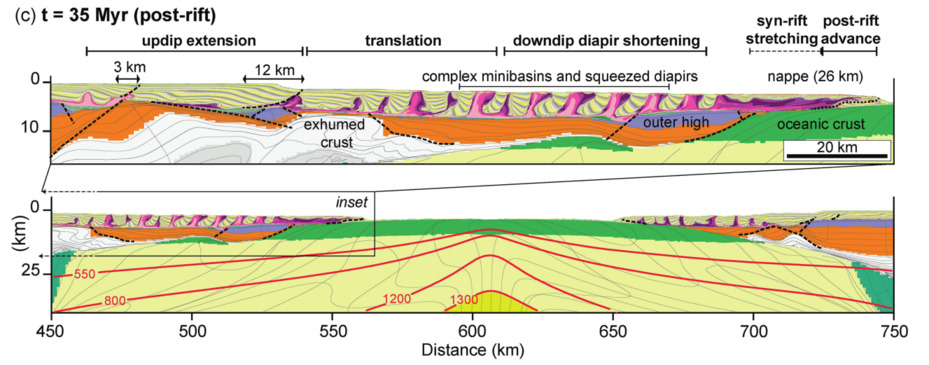
\includegraphics[height=5cm]{images/mycodes/pihg22a_img}
\end{center}

%--------------------------------------------------------------------------------------------------
\item {\it Coupling Crustal-Scale Rift Architecture With Passive Margin
Salt Tectonics: A Geodynamic Modeling Approach}, 
L.M. Pichel, R.S. Huismans, R. Gawthorpe, J.I. Faleide and Th. Theunissen, JGR, 127, 2022. \cite{pihg22b}
\begin{center}
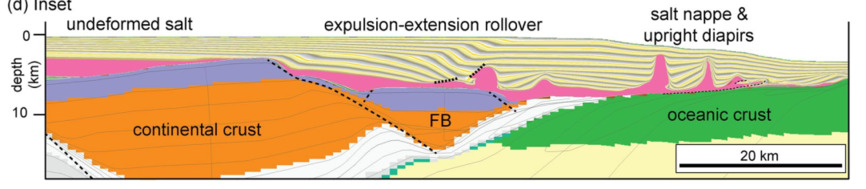
\includegraphics[height=3cm]{images/mycodes/pihg22b_img}
\end{center}

%--------------------------------------------------------------------------------------------------
\item {\it How post-­salt sediment flux and progradation rate
influence salt tectonics on rifted margins: Insights from
geodynamic modelling},
L.M. Pichel, R.S. Huismans, R. Gawthorpe and  J.I. Faleide, Basin Research, 2023. \cite{pihg23}
\begin{center}
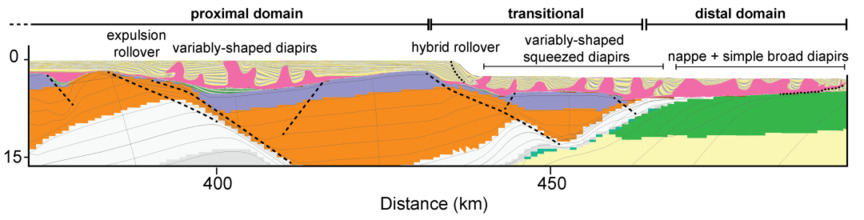
\includegraphics[height=3cm]{images/mycodes/pihg23_img}
\end{center}

\item {\it A Three-Field Formulation for Two-Phase Flow in
Geodynamic Modeling: Toward the Zero-Porosity Limit},
Gang Lu, Dave A. May and Ritske S. Huismans, 
Journal of Geophysical Research: Solid Earth, 2024. \cite{lumh24}


\end{itemize}


%--------------------------------------------------------------------------------------------------
%--------------------------------------------------------------------------------------------------
%--------------------------------------------------------------------------------------------------
%--------------------------------------------------------------------------------------------------

Upon my arrival at Utrecht University in 2012 I started working an a more flexible code, called \elefant, 
which has since very much diverged from \fantom.

\begin{itemize}
\item {\it The effect of obliquity on temperature in subduction zones: insights from 3-D numerical modeling}, 
A. Plunder, C. Thieulot and D.J.J. van Hinsbergen, Solid Earth 9, 759-776, 2018. \url{https://doi.org/10.5194/se-9-759-2018}

\begin{center}
\includegraphics[height=3.5cm]{images/mycodes/pltv18_img}
\end{center}


\item {\it Analytical solution for viscous incompressible Stokes flow in a spherical shell}, 
C. Thieulot, Solid Earth 8, 1181-1191, 2017. \url{https://doi.org/10.5194/se-8-1181-2017}

\begin{center}
\includegraphics[height=3cm]{images/mycodes/thie17_img}
\end{center}



\item  {\it Lithosphere erosion and continental breakup: interaction of extension, plume upwelling and melting}, 
A. Lavecchia, C. Thieulot, F. Beekman, S. Cloetingh and S. Clark, E.P.S.L. 467, p89-98, 2017.

\begin{center}
\includegraphics[height=3cm]{images/mycodes/latv17_img}
\end{center}


\item {\it Benchmarking numerical models of brittle thrust wedges}, 
Susanne J.H. Buiter, Guido Schreurs, Markus Albertz, Taras V. Gerya, Boris Kaus,
Walter Landry, Laetitia le Pourhiet, Yury Mishin, David L. Egholm, Michele Cooke,
Bertrand Maillot, Cedric Thieulot, Tony Crook, Dave May, Pauline Souloumiac, Christopher Beaumont
Journal of Structural Geology 92, p140-177, 2016. \url{https://doi:10.1016/j.jsg.2016.03.003}

\begin{center}
\includegraphics[height=1.8cm]{images/mycodes/busa16_img}
\end{center}


\item {\it A community benchmark for viscoplastic thermal convection in a 2-D square box}, 
N. Tosi, C. Stein, L. Noack, C. Huettig, P. Maierova, H. Samuel, D.R. Davies, C.R. Wilson, S.C. Kramer, C. Thieulot, A. Glerum, M. Fraters, W. Spakman, A. Rozel, P.J. Tackley, Geochem. Geophys. Geosyst. 16, doi:10.1002/2015GC005807, 2015.

\begin{center}
\includegraphics[height=3cm]{images/mycodes/tosn15_img}
\end{center}


\item {\it Dynamics of intraoceanic subduction initiation: 1. Oceanic detachment fault inversion and the formation of supra-subduction zone ophiolites}, M. Maffione, C. Thieulot, D.J.J. van Hinsbergen, A. Morris, O. Pluemper and W. Spakman, Geochem. Geophys. Geosyst. 16, p1753-1770, 2015.

\begin{center}
\includegraphics[height=1.8cm]{images/mycodes/matv15_img}
\end{center}

\item {\it The Geodynamic World Builder: a solution for complex initial conditions in numerical modelling},
M. Fraters, C. Thieulot, A. van den Berg and W. Spakman,
Solid Earth, \url{https://doi.org/10.5194/se-2019-24}, 2019.

\begin{center}
\includegraphics[height=2.8cm]{images/mycodes/frtv19_img}
\end{center}


\end{itemize}


\begin{itemize}
\item {\it GHOST: Geoscientific Hollow Sphere Tessellation}, 
C. Thieulot, Solid Earth, 9, 1169-1177, 2018. \url{https://doi.org/10.5194/se-9-1169-2018}

\begin{center}
\includegraphics[height=3cm]{images/mycodes/shell_HS06}
\includegraphics[height=3cm]{images/mycodes/shell_HS12}
\includegraphics[height=3cm]{images/mycodes/shell_HS20}
\end{center}


title={Long-term coupling and feedback between tectonics and surface processes 
during non-volcanic rifted margin formation},
author={Theunissen, Thomas and Huismans, Ritske S},
journal={Journal of Geophysical Research: Solid Earth},

\end{itemize}



\printbibliography

\end{document}
%%%%%%%%%%%%%%%%%%%%%%%%%%%%%%%%%%%%%%%%%%%%%%%%%%%%%%%%%%%
